% !TEX root
%
% Copyright (c) 2018  UAVCAN Development Team
%

\documentclass{uavcandoc}

\usepackage{multirow}
\usepackage{tabularx}
\usepackage{amsmath}
\usepackage{amsfonts}

% To be removed when ready for publication
\usepackage{draftwatermark}
\SetWatermarkScale{1.2}
\SetWatermarkLightness{0.9}

\urlstyle{same}

\title{Specification v1.0}

\hbadness=10000

\begin{document}
\frontmatter

\begin{titlepage}

\section*{Overview}

UAVCAN is an open lightweight protocol designed for reliable communication in aerospace and robotic applications via
robust vehicle bus networks.

Features:

\begin{itemize}
    \item Democratic network - no bus master, no single point of failure.
    \item Publish/subscribe and request/response (RPC\footnote{Remote procedure call.}) exchange semantics.
    \item Efficient exchange of large data structures with automatic decomposition and reassembly.
    \item Lightweight, deterministic, easy to implement, and easy to validate.
    \item Suitable for deeply embedded, resource constrained, hard real-time systems.
    \item Supports dual and triply modular redundant transports.
    \item Supports high-precision network-wide time synchronization.
    \item The specification and high quality reference implementations in popular programming languages are free,
    open source, and available for commercial use (MIT license).
\end{itemize}

\BeginRightColumn

\section*{Support and feedback}

Information, documentation, and discussions related to UAVCAN are available via the official website at
\href{http://uavcan.org}{uavcan.org}.

\section*{License}

UAVCAN is a standard open to everyone, and it will always remain this way.
No licensing or approval of any kind is necessary for its implementation, distribution, or use.

% The following statement looks a bit archaic, but it is the recommended form according to
% https://creativecommons.org/choose/results-one?license_code=by&amp;jurisdiction=&amp;version=4.0&amp;lang=en
This work is licensed under the Creative Commons Attribution 4.0 International License.
To view a copy of this license, visit \url{http://creativecommons.org/licenses/by/4.0/}
or send a letter to Creative Commons, PO Box 1866, Mountain View, CA 94042, USA.

\begin{center}
    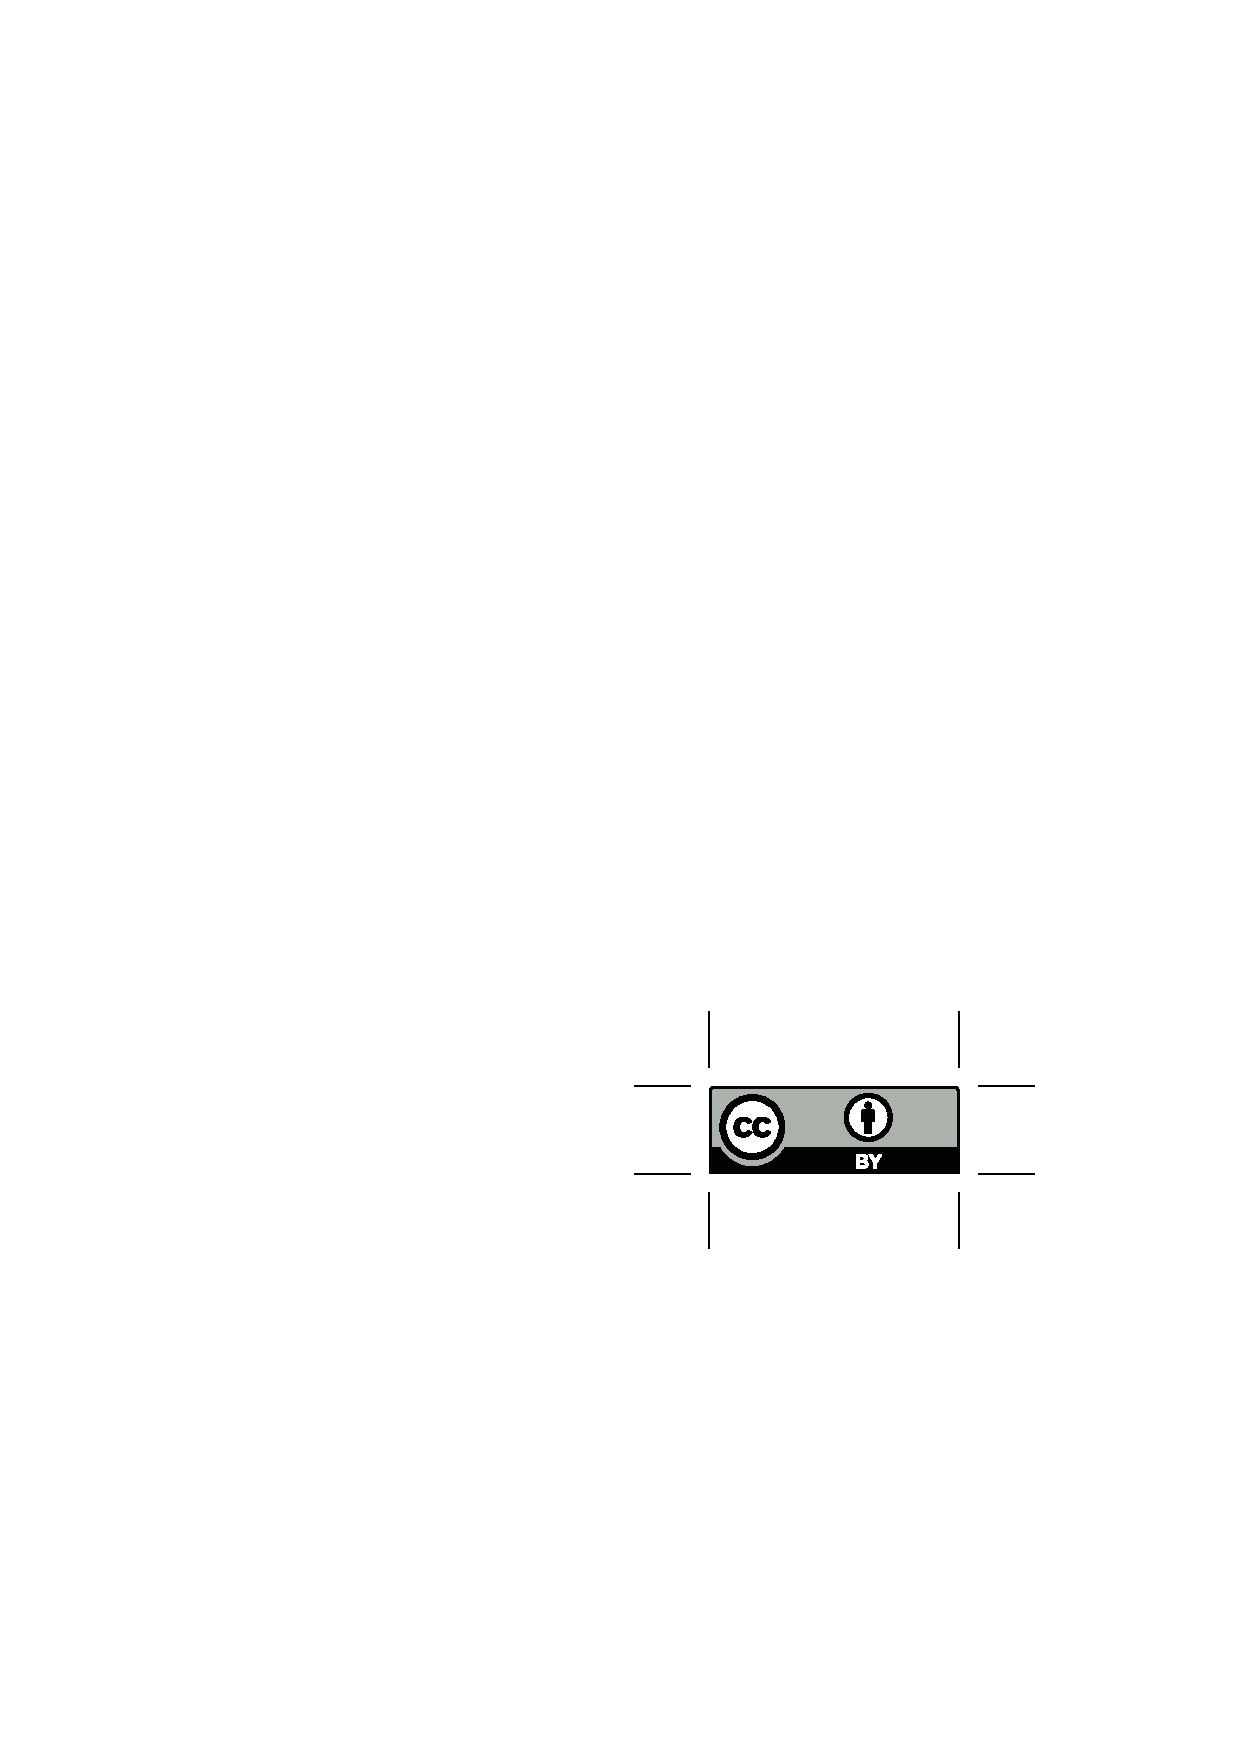
\includegraphics[width=0.3\textwidth]{cc-by}
\end{center}

\BeginRightColumn

\section*{Disclaimer of warranty}

NOTE WELL: This Specification is provided on an ``AS IS'' BASIS, WITHOUT WARRANTIES OR CONDITIONS OF ANY KIND,
express or implied, including, without limitation, any warranties or conditions of
TITLE, NON-INFRINGEMENT, MERCHANTABILITY, or FITNESS FOR A PARTICULAR PURPOSE.

\BeginRightColumn

\section*{Limitation of liability}

In no event and under no legal theory, whether in tort (including negligence), contract, or otherwise,
unless required by applicable law (such as deliberate and grossly negligent acts) or agreed to in writing,
shall any author of this Specification be liable for damages,
including any direct, indirect, special, incidental, or consequential damages of any character arising
from, out of, or in connection with the Specification or the implementation, deployment,
or other use of the Specification (including but not limited to damages for loss of goodwill,
work stoppage, equipment failure or malfunction, injuries to persons,
or any and all other commercial damages or losses),
even if such author has been advised of the possibility of such damages.

\end{titlepage}

\tableofcontents
\BeginRightColumn
\listoftables
\BeginRightColumn
\listoffigures

\mainmatter

\chapter{Introduction}\label{sec:introduction}

This is a non-normative chapter covering the basic concepts that govern development and maintenance of
the specification.

\section{Overview}

UAVCAN is a lightweight protocol designed to provide a highly reliable communication method
supporting publish-subscribe and remote procedure call semantics
for aerospace and robotic applications via robust vehicle bus networks.
It is created to address the challenge of deterministic on-board data exchange between systems and components
of next-generation intelligent vehicles: manned and unmanned aircraft, spacecraft, robots, and cars.

UAVCAN can be approximated as a highly deterministic decentralized object request broker
with a specialized interface description language and a highly efficient data serialization format
suitable for use in real-time safety-critical systems with optional modular redundancy.

The name UAVCAN stands for \emph{Uncomplicated Application-level Vehicular Communication And Networking}.

UAVCAN is a standard open to everyone, and it will always remain this way.
No licensing or approval of any kind is necessary for its implementation, distribution, or use.

The development and maintenance of the UAVCAN specification is governed through the public discussion forum,
software repositories, and other resources available via the website at \href{http://uavcan.org}{uavcan.org}.

\section{Document conventions}

Non-normative text, examples, recommendations, and elaborations that do not directly participate
in the definition of the protocol are contained in footnotes\footnote{This is a footnote.}
or highlighted sections as shown below.

\begin{remark}
    Non-normative sections such as examples are enclosed in shaded boxes like this.
\end{remark}

Code listings are formatted as shown below.
All such code is distributed under the same license as this specification, unless specifically stated otherwise.

\begin{minted}{python}
    # This is a source code listing.
    print('Hello world!')
\end{minted}

A byte is a group of eight (8) bits.

Textual patterns are specified using the standard
POSIX Extended Regular Expression (ERE) syntax;
the character set is ASCII and patterns are case sensitive, unless explicitly specified otherwise.

Type parametrization expressions use subscript notation,
where the parameter is specified in the subscript enclosed in angle brackets:
$\texttt{type}_\texttt{<parameter>}$.

Numbers are represented in base-10 by default.
If a different base is used, it is specified after the number in the subscript:
$\text{BADC0FFEE}_{16} = 50159747054$, $10101_2$.

\section{Design principles}

\begin{description}
    \item[Democratic network] --- There will be no master node.
    All nodes in the network will have the same communication rights; there shall be no single point of failure.

    \item[Facilitation of functional safety] --- A system designer relying on UAVCAN will have the necessary
    guarantees and tools at their disposal to analyze the system and ensure its correct behavior.

    \item[High-level communication abstractions] --- The protocol will support publish/subscribe and remote procedure
    call communication semantics with statically defined and statically verified data types (schema).
    The data types used for communication will be defined in a clear, platform-agnostic way
    that can be easily understood by machines, including humans.

    \item[Facilitation of cross-vendor interoperability] --- UAVCAN will be a common foundation that
    different vendors can build upon to maximize interoperability of their equipment.
    UAVCAN will provide a generic set of standard application-agnostic communication data types.

    \item[Well-defined generic high-level functions] --- UAVCAN will define standard services
    and messages for common high-level functions, such as network discovery, node configuration,
    node software update, node status monitoring\footnote{Which naturally grows into a vehicle-wide
    health monitoring solution.}, network-wide time synchronization, plug-and-play node support, etc.

    \item[Atomic data abstractions] --- Nodes shall be provided with a simple way of exchanging large
    data structures that exceed the capacity of a single transport frame\footnote{A \emph{transport frame} is
    an atomic transmission unit defined by the underlying transport protocol. For example, a CAN frame.}.
    UAVCAN should perform automatic data decomposition and reassembly at the protocol level,
    hiding the related complexity from the application.

    \item[High throughput, low latency, determinism] --- UAVCAN will add a very low overhead to the underlying
    transport protocol, which will ensure high throughput and low latency, rendering the protocol well-suited
    for hard real-time applications.

    \item[Support for redundant interfaces and redundant nodes] --- UAVCAN shall be suitable for use in
    applications that require modular redundancy.

    \item[Simple logic, low computational requirements] --- UAVCAN targets a wide variety of embedded systems,
    from high-performance on-board computers to extremely resource-constrained microcontrollers.
    It will be inexpensive to support in terms of computing power and engineering hours,
    and advanced features can be implemented incrementally as needed.

    \item[Rich data type and interface abstractions] --- an interface description language will be a core part of
    the technology which will allow deeply embedded sub-systems to interface with higher-level systems directly and
    in a maintainable manner while enabling simulation and functional testing.

    \item[Support for various transport protocols] --- UAVCAN will be usable with different transports.
    The standard shall be capable of accommodating other transport protocols in the future.

    \item[API-agnostic standard] --- Unlike some other networking standards, UAVCAN will not attempt to describe
    the application program interface (API). Any details that do not affect the behavior of an implementation
    observable by other participants of the network will be outside of the scope of this specification.

    \item[Open specification and reference implementations] --- The UAVCAN specification will always be open and
    free to use for everyone; the reference implementations will be distributed under the terms of
    the permissive MIT License or released into the public domain.
\end{description}

\section{Capabilities}

The maximum number of nodes per logical network is dependent on the transport protocol in use,
but it is guaranteed to be not less than 128.

UAVCAN supports an unlimited number of composite data types,
which can be defined by the specification (such definitions are called ``standard data types'')
or by others for private use or for public release
(in which case they are said to be ``application-specific'' or ``vendor-specific''; these terms are equivalent).
There can be up to 256 major versions of a data type, and up to 256 minor versions per major version.
More information is provided in chapter \ref{sec:dsdl}.

UAVCAN supports 32768 message subject identifiers for publish/subscribe exchanges and
512 service identifiers for remote procedure call exchanges.
A small subset of these identifiers is reserved for the core standard and for publicly released vendor-specific types.
More information is provided in chapter \ref{sec:application_layer}.

UAVCAN supports at least\footnote{Depending on the transport protocol.} eight distinct communication priority levels,
defined in section \ref{sec:transfer_prioritization}.
Within each priority level different types of transfers, messages, and services are
prioritized in a well-defined, deterministic manner.

The list of transport protocols supported by UAVCAN is provided in chapter \ref{sec:transport_layer}.
Non-redundant, doubly-redundant and triply-redundant transports are supported.
More information on the physical layer and standardized physical connectivity options
is provided in chapter \ref{sec:physical_layer}.
Additional transport and physical layers may be added in future revisions of the protocol.

\section{Public regulated data types}

This section talks about general management policies.
The related technical aspects are covered in chapters~\ref{sec:basic_concepts} and~\ref{sec:dsdl}.

The UAVCAN maintainers are charged with maintaining and advancing the set of
public regulated data types based on the input from adopters.
This feedback is gathered via the online discussion and collaboration websites
which are open to the general public and available through \href{http://uavcan.org}{uavcan.org}.

The set of standard data types is a subset of public regulated data types and is an integral part of the specification;
however, there is only a very small subset of required standard data types needed to implement the protocol.
A larger set of optional data types are defined to create a standardized data exchange environment
supporting the interoperability of COTS\footnote{Commercial off-the-shelf equipment.}
equipment manufactured by different vendors.
See chapter \ref{sec:application_layer} for more information.

Within the same major version of the specification,
the set of public regulated data type definitions can be modified only in the following ways:

\begin{itemize}
    \item A new data type can be added, as long as it doesn't conflict with any of the existing data types.

    \item An existing data type can be modified, as long as its version number is updated accordingly
    and all backward compatibility guarantees are respected.

    \item An existing data type or a particular major version of it can be declared deprecated.
    \begin{itemize}
        \item Once declared deprecated, the data type will be maintained for at least two more years.
        After this period, its regulated fixed port-ID (if defined) may be reused for
        an incompatible data type definition.
        The maintainers will be striving to postpone the reuse of regulated port identifiers as much as
        possible in order to minimize the possibility of unintended conflicts.

        \item Deprecation will be indicated in the DSDL definition and announced via the discussion forum.
    \end{itemize}
\end{itemize}

A link to the repository containing the set of default DSDL definitions can be found on the official website.

\section{Referenced sources}

The UAVCAN specification contains references to the following sources:

\begin{itemize}
    \item CiA 801 --- Application note --- Automatic bit rate detection.
    \item CiA 103 --- Intrinsically safe capable physical layer.
    \item CiA 303 --- Recommendation --- Part 1: Cabling and connector pin assignment.
    \item IEEE 754 --- Standard for binary floating-point arithmetic.
    \item ISO 11898-1 --- Controller area network (CAN) --- Part 1: Data link layer and physical signaling.
    \item ISO 11898-2 --- Controller area network (CAN) --- Part 2: High-speed medium access unit.
    \item ISO/IEC 10646 --- Universal Coded Character Set (UCS).
    \item ISO/IEC 14882 --- Programming Language C++.
    \item ``Implementing a Distributed High-Resolution Real-Time Clock using the CAN-Bus'', M. Gergeleit and H. Streich.
    \item ``In Search of an Understandable Consensus Algorithm (Extended Version)'', Diego Ongaro and John Ousterhout.
    \item \href{http://semver.org}{semver.org} - Semantic versioning specification.
    \item IEEE Std 1003.1 --- IEEE Standard for Information Technology --
    Portable Operating System Interface (POSIX) Base Specifications.
    \item IETF RFC2119 --- Key words for use in RFCs to Indicate Requirement Levels.
\end{itemize}

\section{Revision history}

\subsection{v1.0-alpha}

This is the initial version of the document.
The discussions that shaped the initial version are available on the public UAVCAN discussion forum.

This version is to be followed by \emph{v1.0} upon completion of the formal standardization process
in one of the standard bodies.
Meanwhile, the document may undergo modifications that are either non-essential (e.g., minor conventions or wording)
or that are mandatory to ensure the long-term success of the technology (e.g., resolution of design mistakes).

%\subsection{v1.0}
% Hello world!

\chapter{Basic concepts}\label{sec:basic_concepts}

\section{Main principles}

\subsection{Communication}

\subsubsection{Architecture}

A UAVCAN network is a decentralized peer network, where each peer (node) has a unique
numeric identifier\footnote{Here and elsewhere in this specification, \emph{ID} and \emph{identifier} are used
interchangeably unless specifically indicated otherwise.}
--- \emph{node ID} --- ranging from 1 to 127, inclusively.
Nodes of a UAVCAN network can communicate using the following communication methods:

\begin{description}
    \item[Message publication] --- The primary method of data exchange with one-to-many publish/subscribe semantics.
    \item[Service invocation] --- The communication method for one-to-one request/response
    interactions\footnote{Like remote procedure call (RPC).}.
\end{description}

For each type of communication, a predefined set of data types is used,
where each data type has a unique name.
Additionally, every data type definition has a pair of major and minor version numbers,
which enable data type definitions to evolve in arbitrary ways while ensuring a well-defined
migration path if backward-incompatible changes are introduced.
Some data types are standard and defined by the protocol specification (of which only a small
subset are required); others may be specific to a particular application or vendor.

\subsubsection{Subjects and services}

Message exchanges between nodes are grouped into \emph{subjects} by their semantic meaning.
Message exchanges belonging to the same subject use same message data type down to the major version
(minor versions are allowed to differ) and pertain to same function or process within the system.

Request/response exchanges between nodes are grouped into \emph{services} by their semantic meaning,
like messages are grouped into subjects.
Requests and their corresponding responses that belong to the same service use same service data type down to
the major version (minor versions are allowed to differ; as a consequence, the minor data type version number
of a service response may differ from that of its corresponding request) and pertain to same function.

Each message subject is identified by a unique natural number -- a \emph{subject ID};
likewise, each service is identified by a unique \emph{service ID}.
An umbrella term \emph{port ID} is used to refer either to a subject ID or to a service ID
(port identifiers have no direct manifestation in the construction of the protocol,
but they are convenient for discussion).

\subsection{Data types}

\subsubsection{Data type definitions}

Message and service data types\footnote{Data types are the core concept of UAVCAN.}
are defined using the \emph{data structure description language} (DSDL) (chapter \ref{sec:dsdl}).
A DSDL definition specifies the name, major version, minor version, the data structure,
and an optional predefined port ID of the data type.
Message data types always contain exactly one data structure, whereas
service data types contain two data structures: one for request, and the other for response.

If a port identifier is specified in a data type definition, such identifier is said to be a
\emph{fixed port identifier}
(by inheritance, the same naming principle applies to \emph{fixed subject ID} and \emph{fixed service ID}).
A data type can be used with an arbitrary number of different port identifiers assigned on a per-application basis,
but not more than one fixed port identifier.

\subsubsection{Regulation}

Data type definitions can be created by the UAVCAN specification maintainers or by its users,
such as equipment vendors or application designers.
Irrespective of the origin, data types can be included into the set of data type definitions maintained
and distributed by the UAVCAN specification maintainers;
definitions belonging to this set are termed \emph{regulated data type definitions}.
The specification maintainers undertake to keep regulated definitions well-maintained and may occasionally
amend them and release new versions, if such actions are believed to benefit the protocol.
User-created (i.e., vendor-specific or application-specific) data type definitions that are
not included into the aforementioned set are called \emph{unregulated data type definitions}.

Unregulated definitions that are made available for reuse by others are called
\emph{unregulated public data type definitions};
those that are kept closed-source for private use by their authors are called
\emph{(unregulated) private data type definitions}\footnote{The word \emph{``unregulated''} is redundant
because private data types cannot be regulated, by definition.
Likewise, all regulated definitions are public, so the word \emph{``public''} can be omitted.}.

Data type definitions authored by the specification maintainers for the purpose of supporting and advancing
this specification are called \emph{standard data type definitions}.
All standard data type definitions are regulated.

Fixed port identifiers can be used only with regulated data type definitions or with private definitions.
Fixed port identifiers must not be used with public unregulated data types,
since that is likely to cause unresolvable port identifier collisions\footnote{
    Any system that relies on data type definitions with fixed port identifiers provided by
    an external party (i.e., the data types and the system in question are designed by different parties)
    runs the risk of encountering port identifier conflicts that cannot be resolved without resorting to help
    of such external party, since the designers of the system do not have control of their fixed port identifiers.
    This is why the specification strongly discourages the use of fixed unregulated private port identifiers.
    If a data type definition is ever disclosed to any other party (i.e., a party that did not author it)
    or to the public at large, such data type should be devoid of a fixed port identifier.
}.
This restriction shall be followed at all times by all compliant implementations and
systems\footnote{
    In general, private unregulated fixed port identifiers are collision-prone by their nature, so they should
    be avoided unless there are very strong reasons for their usage and the authors fully understand the risks.
}.

\begin{UAVCANSimpleTable}{Data type taxonomy}{|l|X|X|}
    & Regulated & Unregulated \\
    \bfseries{Public}
    &
    Standard and contributed (e.g., vendor-specific) definitions.\newline
    Fixed port identifiers are allowed; they are called \emph{``regulated port ID''}.
    &
    Definitions distributed separately from the UAVCAN specification.\newline
    Fixed port identifiers are \emph{not allowed}.
    \\

    \bfseries{Private}
    &
    Nonexistent category.
    &
    Definitions that are typically not available to anyone except their authors.\newline
    Fixed port identifiers are permitted (although not recommended) as long as the definition is only used by
    its authors; they are called \emph{``unregulated fixed port ID''}.
    \\
\end{UAVCANSimpleTable}

DSDL processing tools shall prohibit unregulated fixed port identifiers by default,
unless they are explicitly configured otherwise.

Each of the two sets of valid port identifiers (which are subject identifiers and port identifiers) are
segregated into three categories: application-specific (i.e., non-fixed or unregulated) identifiers,
regulated non-standard port identifiers, and standard port identifiers.
Fixed unregulated port identifiers can be allocated in the same range where application-specific identifiers are.
The ranges are documented in chapter \ref{sec:application_layer}.

Data type authors that desire to release regulated data type definitions or contribute to the standard data
type set should contact the UAVCAN maintainers for coordination.
The maintainers will choose unoccupied fixed port identifiers for use with the new definitions, if necessary.
Since the set of regulated definitions is maintained in a highly centralized manner,
it can be statically ensured that no identifier collisions will take place within it;
also, since the identifier ranges used with regulated definitions are segregated from the rest,
regulated port ID will not conflict with any other compliant UAVCAN node or system\footnote{
    The motivation for the prohibition of fixed port identifiers in unregulated public data types is
    derived directly from the above: since there is no central repository of unregulated definitions,
    collisions would be likely to happen, which would be extremely damaging to the ecosystem.
}.

\subsubsection{Serialization}

A DSDL description can be used to automatically generate the serialization and deserialization code
for every defined data type in a particular programming language.
Alternatively, a DSDL description can be used to construct appropriate serialization code manually by a human.
DSDL ensures that the worst case memory footprint and computational complexity per data type
are constant and easily predictable.

Serialized message and service data structures are exchanged by means of the transport
layer (chapter \ref{sec:transport_layer}), which implements automatic decomposition of
long transfers into several transport frames\footnote{Here and
elsewhere, a \emph{transport frame} means a block of data that can be atomically exchanged
over the transport layer network, e.g., a CAN frame.} and reassembly from these transport frames
back into a single atomic data block, allowing nodes to exchange data structures of
arbitrary size.

\subsection{High-level functions}

On top of the standard data types, UAVCAN defines a set of standard high-level functions including:
node health monitoring, node discovery, time synchronization, firmware update,
plug-and-play node support, and more.
For more information see chapter \ref{sec:application_layer}.

\begin{figure}[hbt]
    \centering
    \begin{tabular}{|c|c|l|c|l|c|}
        \hline
        \multicolumn{6}{|c|}{Applications} \\ \hline

        \qquad{} & Required functions &
        \qquad{} & Standard functions &
        \qquad{} & Custom functions \\
        \cline{2-2} \cline{4-4} \cline{6-6}

        \multicolumn{2}{|c|}{Required data types} &
        \multicolumn{2}{c|}{Standard data types} &
        \multicolumn{2}{c|}{Custom data types} \\ \hline

        \multicolumn{6}{|c|}{Serialization} \\ \hline

        \multicolumn{6}{|c|}{Transport} \\ \hline
    \end{tabular}
    \caption{UAVCAN architectural diagram.\label{fig:architecture}}
\end{figure}

\section{Message publication}

Message publication refers to the transmission of a serialized data structure over the network to other nodes.
This is the primary data exchange mechanism used in UAVCAN;
it is functionally similar to raw data exchange with minimal overhead,
additional communication integrity guarantees, and automatic decomposition and reassembly of long payloads
across multiple transport frames.
Typical use cases may include transfer of the following kinds of data (either cyclically or on an ad-hoc basis):
sensor measurements, actuator commands, equipment status information, and more.

Information contained in a published message is summarized in the table \ref{table:published_message_info}.

\begin{UAVCANSimpleTable}{Published message properties}{|l X|}\label{table:published_message_info}
    Property        & Description \\
    Payload         & The serialized message data structure. \\
    Subject ID      & Numerical identifier that indicates how the information should be interpreted. \\
    Source node ID  & The node ID of the transmitting node (excepting anonymous messages). \\
    Transfer ID     & A small overflowing integer that increments with every transfer
                      of this message type from a given node. Used for message sequence monitoring,
                      multi-frame transfer reassembly, and elimination of transport frame duplication errors
                      for single-frame transfers. Additionally, Transfer ID is crucial for automatic
                      management of redundant transport interfaces. The properties of this field are explained in
                      detail in the chapter \ref{sec:transport_layer}. \\
\end{UAVCANSimpleTable}

\subsection{Anonymous message publication}

Nodes that don't have a unique node ID can publish only \emph{anonymous messages}.
An anonymous message is different from a regular message in that it doesn't contain a source node ID,
and that it can't be decomposed across several transport frames.

UAVCAN nodes will not have an identifier initially until they are assigned one,
either statically (which is generally the preferred option for applications where a high degree of
determinism and high safety assurances are required) or automatically (i.e., plug-and-play).
Anonymous messages are particularly useful for the plug-and-play feature,
which is explored in detail in chapter~\ref{sec:application_layer}.

Anonymous messages cannot be decomposed into multiple transport frames,
meaning that their payload capacity is limited to that of a single transport frame.
More info is provided in chapter~\ref{sec:transport_layer}.

\section{Service invocation}

Service invocation is a two-step data exchange operation between exactly two nodes: a client and a server.
The steps are\footnote{The request/response semantic is facilitated by means of hardware (if available)
or software acceptance filtering and higher-layer logic.
No additional support or non-standard transport layer features are required.}:

\begin{enumerate}
    \item The client sends a service request to the server.
    \item The server takes appropriate actions and sends a response to the client.
\end{enumerate}

Typical use cases for this type of communication include:
node configuration parameter update, firmware update, an ad-hoc action request, file transfer,
and other functions of similar nature.

Information contained in service requests and responses is summarized in the
table \ref{table:service_req_resp_info}.

\begin{UAVCANSimpleTable}{Service request/response properties}{|l X|}\label{table:service_req_resp_info}
    Property        & Description \\
    Payload         & The serialized request/response data structure. \\
    Service ID      & Numerical identifier that indicates how the service should be handled. \\
    Client node ID  & Source node ID during request transfer, destination node ID during response transfer. \\
    Server node ID  & Destination node ID during request transfer, source node ID during response transfer. \\
    Transfer ID     & A small overflowing integer that increments with every call
                      of this service type from a given node. Used for request/response matching,
                      multi-frame transfer reassembly, and elimination of transport frame duplication errors
                      for single-frame transfers. Additionally, Transfer ID is crucial for automatic
                      management of redundant transport interfaces. The properties of this field are explained in
                      detail in the chapter \ref{sec:transport_layer}. \\
\end{UAVCANSimpleTable}

Both the request and the response contain same values for all listed fields except payload,
where the content is application-defined.
Clients match responses with corresponding requests using the following fields:
service ID, client node ID, server node ID, and transfer ID.

\chapter{Data structure description language}\label{sec:dsdl}

The data structure description language (DSDL) is used to define data structures for exchange via the network.
DSDL definitions are used to automatically (or manually) generate the message or service
serialization/deserialization code in a particular programming language.
A tool that automatically generates source code from DSDL definition files is called a \emph{DSDL compiler}.

\section{File hierarchy}

Each DSDL definition file specifies exactly one data structure that can be used for message broadcasting,
or a pair of structures that can be used for service invocation (request and response).

A DSDL source file is named using the \emph{short data type name},
the semantic version number pair (major and minor; see the section \ref{sec:dsdl_versioning}
for more information on data type versioning),
and the \emph{default data type ID} (if needed) as shown
below\footnote{In this declaration, the mandatory parts are surrounded with angle brackets,
and the optional parts are surrounded with square brackets.}:

\verb|[default DTID.]<short name>.<major version number>.<minor version number>.uavcan|

Every defined data structure is contained in a namespace,
which may in turn be \emph{nested} within another namespace.
A namespace that is not nested in another namespace is called a \emph{root namespace}.
For example, all standard data types are contained in the root namespace \verb|uavcan|,
which contains nested namespaces, such as \verb|protocol|.

The namespace hierarchy is mapped directly to the file system directory structure,
as shown in the example below:

\begin{minted}[linenos=false]{text}
uavcan/                           <- Root namespace
    equipment/                    <- Nested namespace
        ...
    protocol/                     <- Nested namespace
        341.NodeStatus.1.0.uavcan <- Data type "uavcan.protocol.NodeStatus" v1.0 with default DTID 341
        ...
    Timestamp.uavcan              <- Data type "uavcan.Timestamp", default DTID is not assigned
\end{minted}

Notes:

\begin{itemize}
    \item It is not necessary to explicitly define a default data type ID for non-standard data types
          (i.e., for vendor-specific or application-specific data types).
    \begin{itemize}
        \item If the default data type ID is not defined by the DSDL definition,
              it will need to be assigned by the application at run time.
        \item All standard data types have default data type ID values defined.
    \end{itemize}

    \item Data type names are case sensitive, i.e., names \verb|foo.Bar| and \verb|foo.bar| are considered different.
          Names that differ only in case should be avoided, because it may cause problems on file systems that are not
          case-sensitive.

    \item Data types may contain nested data structures.
    \begin{itemize}
        \item Some data structures may be designed for such nesting only,
              in which case they are not required to have a dedicated data type ID at all
              (neither default nor runtime-assigned).
    \end{itemize}

    \item \emph{Full data type name} is a unique identifier of a data type constructed from the root namespace,
          all nested namespaces (if any), and the short data type name, joined via the dot symbol (\verb|.|),
          e.g., \verb|uavcan.protocol.file.Read|.
    \begin{itemize}
        \item The total length of the full data type name must not exceed 80 characters.
        \item Refer to the naming rules below for the limitations imposed on the character set.
    \end{itemize}
\end{itemize}

\subsection{Service data types}

Since a service invocation consists of two independent network data exchange operations,
the DSDL definition for a service must define two structures:

\begin{description}
    \item[Request part] - for the request transfer (client to server).
    \item[Response part] - for the response transfer (server to client).
\end{description}

Both request and response structures are contained within the same DSDL definition file,
separated by a special statement as defined in the section \ref{sec:dsdl_syntax}.

Service invocation data structures cannot be nested into other structures.

\section{Syntax}\label{sec:dsdl_syntax}

A data structure definition is a collection of statements.
Each statement is located on a separate line.
Lines are separated with the ASCII line feed character (\verb|\n|, code 10),
or with a sequence consisting of the ASCII carriage return character followed by the ASCII line feed character
(\verb|\r\n|, code 13 and 10, respectively).

The following types of statements are defined:

\begin{description}
    \item[Attribute] - used to define entities of the data type, such as data fields and associated constants.
    \item[Directive] - directives provide instructions to the DSDL compiler.
    \item[Service response marker] - separates the request and response parts of a service data type definition.
\end{description}

An attribute defines one of the following:

\begin{description}
    \item[Field] - a variable that can be modified by the application and exchanged via the network.
    \item[Associated Constant] - an immutable value that does not participate in network exchange.
\end{description}

DSDL source files may also contain human-readable comments, which are ignored by the compiler.

A message data type definition may contain the following entities:

\begin{itemize}
    \item Attribute definitions
    \item Directives
    \item Comments
\end{itemize}

A service data type definition may contain the following entities:

\begin{itemize}
    \item Request part attribute definitions
    \item Response part attribute definitions
    \item Request part directives
    \item Response part directives
    \item Comments
    \item Service response marker (always exactly one marker) (section \ref{sec:dsdl_service_response_marker})
\end{itemize}

Unless specifically stated otherwise,
directives apply only to the part of the service type definition where they are defined,
not crossing the boundary of the service response marker.


\subsection{Constant expressions}\label{sec:dsdl_constant_expressions}
A valid constant expression is either just a constant, or an expression that results in a constant.
Such expression is given in infix notation,
this means \texttt{A <op> B} for binary operators and \texttt{<op> A} for unary operators.
A comprehensive table of legal operations on types is defined below,
the order of the table also defines the order of precedence between operations.

\begin{UAVCANSimpleTable}{Operators for constant expressions}{|c c c c c l|} \label{table:dsdl_const_operators}
Precedence & Op & A & B & Res & Description \\
1 & \texttt{!}    &  \texttt{const bool}   & N/A                  & \texttt{const bool}    & Logical not \\


2 & \texttt{*}    & \texttt{const int}    & \texttt{const int}   & \texttt{const int}     & Integer multiplication \\
2 & \texttt{/}    & \texttt{const int}    & \texttt{const int}   & \texttt{const int}     & Integer division \\
2 & \texttt{\%}   & \texttt{const int}    & \texttt{const int}   & \texttt{const int}     & Integer remainder \\

2 & \texttt{*}    & \texttt{const float}  & \texttt{const float} & \texttt{const float}   & IEE754 multiplication \\
2 & \texttt{/}    & \texttt{const float}  & \texttt{const float} & \texttt{const float}   & IEE754 division \\

2 & \texttt{\%} & \texttt{\{const int\}}  & \texttt{const int}   & \texttt{\{const int\}} & Element-wise int remainder\\


3 & \texttt{+}    & \texttt{const float}  & \texttt{const float} & \texttt{const float}   & IEEE754 sum \\
3 & \texttt{-}    & \texttt{const float}  & \texttt{const float} & \texttt{const float}   & IEEE754 difference \\

3 & \texttt{+}    & \texttt{const int}    & \texttt{const int}   & \texttt{const int}     & Integer sum \\
3 & \texttt{-}    & \texttt{const int}    & \texttt{const int}   & \texttt{const int}     & Integer difference \\


4 & \texttt{==}   & \texttt{const int}    & \texttt{const int}   & \texttt{const bool}    & Integer equality \\
4 & \texttt{!=}   & \texttt{const int}    & \texttt{const int}   & \texttt{const bool}    & Integer inequality \\
4 & \texttt{==}   & \texttt{const bool}   & \texttt{const bool}  & \texttt{const bool}    & Boolean equality \\
4 & \texttt{!=}   & \texttt{const bool}   & \texttt{const bool}  & \texttt{const bool}    & Boolean inequality \\
4 & \texttt{==}   & \texttt{const char}   & \texttt{const char}  & \texttt{const bool}    & Character equality \\
4 & \texttt{!=}   & \texttt{const char}   & \texttt{const char}  & \texttt{const bool}    & Character inequality \\
4 & \texttt{==}   & \texttt{\{T\}}        & \texttt{\{T\}}       & \texttt{const bool}    & Set equality \\
4 & \texttt{!=}   & \texttt{\{T\}}        & \texttt{\{T\}}       & \texttt{const bool}    & Set inequality \\


5 & \texttt{\&\&} & \texttt{const bool}   & \texttt{const bool}  & \texttt{const bool}    & Logical and \\
5 & \texttt{\&\&} & \texttt{const bool}   & \texttt{const bool}  & \texttt{const bool}    & Logical or
\end{UAVCANSimpleTable}


\subsection{Attribute definition}
Attribute definitions are instructions to the DSDL compiler
that defines different aspects of the enclosing type definition.
Field definitions adds a field to the datatype and serialization code,
a field definition follows the following declaration patterns:
\begin{itemize}
    \item \verb|cast_mode field_type field_name|
\end{itemize}

Void definitions instructs the serialization code to discard a small chunk of bits, it is declared as following:
\begin{itemize}
    \item \verb|void_type|
\end{itemize}

Associated constant definitions instructs the compiler to create a constant associated with the enclosing type,
the following declaration pattern applies:
\begin{itemize}
    \item \verb|associated_constant_type associated_constant_name = constant_expression|
\end{itemize}

Each component of the specified patterns is reviewed in detail below.

\subsubsection{Field type}

A field type declaration can be either a primitive data type (defined in section \ref{sec:dsdl_primitive_data_types}),
an array type (defined in section \ref{sec:dsdl_array_data_types}) or a nested data structure.

A primitive data type is referred simply by its name, e.g., \verb|float16|, \verb|bool|.

A nested data structure is referred by its name and the version number,
separated by the ASCII dot (full stop) character.
The name can be either the full name or the short name.
The latter option is permitted only if the referred data type is located in the same namespace as
the referring data type.
The version number can be either the major version number, or both the major and the minor version
numbers separated by the ASCII dot (full stop) character.
In the former case, the highest available minor version number is implied.
Consider the following examples,
where all of the declarations refer to the same nested data type, assuming that the referring definition is
located in the namespace \verb|uavcan.protocol|:

\begin{minted}[linenos=false]{text}
NodeStatus.1
NodeStatus.1.0
uavcan.protocol.NodeStatus.1
uavcan.protocol.NodeStatus.1.0
\end{minted}

An array field uses its type constructor to specify the type e.g.,
\verb|float16[5]|, \verb|Type.0.1[<10]| \verb|Type2.0[<=12]|.

\subsubsection{Field name and associated constant name}

For a message data type, all attributes must have a unique name within the data type definition.

For a service data type, all attributes must have a unique name within the same part (request/response) of
the data type definition.
In other words, service type attributes can have the same name as long as they are separated by
the service response marker (section \ref{sec:dsdl_service_response_marker}).

Restrictions on the character set and further information are provided in the section \ref{sec:dsdl_naming_rules}.

\subsubsection{Cast mode}

Cast mode defines the rules of conversion from native values of a particular programming language
to serialized field values.
Cast mode may be left undefined, in which case the default will be used.
Cast mode cannot be specified for nested data structures and void field types.
The possible cast modes are defined below.

\begin{itemize}
    \item \verb|saturated| - this is the default cast mode,
          which will be used if the attribute definition does not specify the cast mode explicitly.
          For integers, it prevents an integer overflow, replacing it with saturation -
          for example, an attempt to write 0x44 to a 4-bit field
          will result in a bit field value of 0x0F.
          For floating point values, it prevents overflow when casting to a lower precision floating point
          representation - for example, 65536.0 will be converted to a \verb|float16| as 65504.0;
          infinity will be preserved.
    \item \verb|truncated| - for integers, discards the excessive most significant bits;
          for example, an attempt to write 0x44 to a 4-bit field will produce 0x04.
          For floating point values, overflow during downcasting will produce an infinity.
\end{itemize}

\subsubsection{Associated Constant definition}\label{sec:dsdl_constant_definition}
A constant attribute definition both defines a constant to be used in const evaluation context,
and instructs the DSDL compiler to generate an associated constant.

Whenever the constant is used in a context where a const type is expected, its const type is used.
As a result, associated constant definitions can be used for assertions,
define array lengths, and defining other associated constants.

When all constant evaluations are finished and the DSDL is to be compiled,
the resulting associated const will have the type defined by the \verb|associated_constant_type|.
Since the range of the associated const types ranges are subsets of the their compatible const counterparts ranges,
checks related to data loss must be done before/when converting from the const type to the associated const type.
If the bounds check fails,
the DSDL compiler must refuse to compile the type encapsulating the associated constant definition.

The compatbility between const types and associated const types,
and the concrete checks that must be performed are as follows:

\begin{UAVCANSimpleTable}{Compatibility between associated const and const type}{|l l l|}
    \label{table:dsdl_associated_const_compatibility}
    Const type & Associated Const type & Conversion checks \\
    \texttt{const bool} &
        \texttt{bool} &
        Only Type checking, will always convert successfully to \texttt{bool}. \\

    \texttt{const int} &
        \texttt{int\textbf{X}} &
        Type checking, Bounds checking. \\

    \texttt{const int} &
        \texttt{uint\textbf{X}} &
        Type checking, Bounds checking. \\

    \texttt{const float} &
        \texttt{float\textbf{X}} &
        Type checking, Bounds checking. \\

    \texttt{const char} &
        \texttt{uint8 | uint7} &
        Only Type checking, can always be converted to both \texttt{uint8} and \texttt{uint7}.
\end{UAVCANSimpleTable}

Note that associated constants do not affect the serialized data layout as they are never exchanged via the network.

\subsubsection{Void type}

Void type is a special field type that is intended for data alignment purposes.
The specification defines 64 distinct void types as follows:

\begin{itemize}
    \item \verb|void1| - 1 padding bit;
    \item \verb|void2| - 2 padding bits;
    \item \ldots
    \item \verb|void63| - 63 padding bits;
    \item \verb|void64| - 64 padding bits.
\end{itemize}

A field of a void type does not have a name and its cast mode cannot be specified.
During message serialization, all void fields are filled with zero bits;
during deserialization, the contents of void fields should be ignored.

\subsection{Directives}\label{sec:dsdl_directives}

A directive is a single case-sensitive word starting with an ASCII "at sign" character (\verb|@|),
possibly followed by space-separated arguments:

\begin{minted}[linenos=false]{text}
@directive
@directive arg1 arg2
\end{minted}

All valid directives are documented in this section.

\subsubsection{Union}

Keyword: \verb|@union|.

This directive instructs the DSDL compiler that the current message or the current part of a service data type
(request or response) is a \emph{tagged union}.
A tagged union is a data structure that may encode any one of its fields at a time.
Such a data structure contains one implicit field - the \emph{union tag} - that indicates which particular
field the data structure is holding at the moment.
Unions are required to have at least two fields.

This directive must be placed before the first attribute definition.

\subsubsection{Deprecated}

Keyword: \verb|@deprecated|.

This directive notifies the DSDL compiler that the current data type definition
is scheduled for removal in the future.
Note that it applies to the current \emph{definition} and not to the data type as a whole,
meaning that only the current version is affected, while newer versions,
if available, are not to be considered deprecated unless also marked with this directive.

This directive must be placed before the first attribute definition.
In the case of service data types, this directive must be placed before the first
attribute definition of the request part.

The DSDL compiler can leverage this directive to amend auto-generated entities with
deprecation markers appropriate to the target programming language;
e.g. \verb|[[deprecated]]| in C++, \verb|DeprecationWarning| in Python, and so on.

As explained in the section \ref{sec:dsdl_versioning},
there are circumstances when the DSDL compiler is required to assume implicit deprecation,
as if the \verb|@deprecated| directive was provided in the definition source.

\subsubsection{Assertions}

Keyword: \verb|@assert <constant expression>|.

This directive checks a property that must hold for compilation to succeed.
The provided constant expression must evaluate into a value to type \verb|const bool|.
If the value is \verb|true| the assertion check will pass and the resulting type should be considered valid,
if the value is \verb|false| the resulting type must be considered invalid, and steps must be taken to avoid usage.
Both checking the assertions before compilation and compiling the assertions into compile time assertions in the
resulting languages is considered legal way to handle this as long as it results in no way to use the resulting type.

Keywords that are interesting in relation to assertions are given below.
To allow both earlier described ways of assertions checking,
they are designed in a way such that a DSDL compiler can substitute them for their value early on.
This allow all assertion checking to be done at a separate pass before compilation.
They can also be compiled into values used in target language compile time assertions in the resulting type definition.

\begin{UAVCANSimpleTable}{Compatibility between associated const and const type}{|l l|}
\textbf{Keyword} & \textbf{Description} \\
\texttt{offset}  & The set of possible bit offsets when serializing.
\end{UAVCANSimpleTable}

\subsection{Comments}

A DSDL description may contain comments starting from the ASCII number sign (\verb|#|)
up until the end of the current line.
Comments are ignored by DSDL compilers.

\subsection{Service response marker}\label{sec:dsdl_service_response_marker}

A service response marker separates the request and response parts of a service data type definition.
The marker consists of three ASCII minus symbols (\verb|-|) in a row on a dedicated line:

\begin{minted}[linenos=false]{text}
---
\end{minted}

The request part precedes the marker, and the response part follows the marker.
The presence of a service response marker indicates that the current definition is a
service type definition rather than a message type definition.

\section{Built in data types}

The following types are assumed to be built-in.
They can be directly referenced from any data type of any namespace.

\subsection{Primitive data types}\label{sec:dsdl_primitive_data_types}

The primitive data types are the most basic building blocks for defining complex types.
The DSDL compiler should implement these types using the native types of the target programming language.
An example mapping to native types is given here for C/C++.

\begin{UAVCANSimpleTable}{Primitive data types}{|l l l X|}\label{table:dsdl_primitive_data_types}
    Name                    & Bit length    & Possible representation in C/C++  & Value range \\
    \texttt{bool}           & $1$
                            & \texttt{bool} (can be optimized for bit arrays)
                            & $\{0, 1\}$
                            \\
    \texttt{int\textbf{X}}  & $2 \le{} \text{X} \le 64$
                            & \texttt{int8\_t}, \texttt{int16\_t}, \texttt{int32\_t}, \texttt{int64\_t}
                            & $\lbrack -\frac{2^\text{X}}{2}, \frac{2^\text{X}}{2} - 1\rbrack$
                            \\
    \texttt{uint\textbf{X}} & $2 \le{} \text{X} \le 64$
                            & \texttt{uint8\_t}, \texttt{uint16\_t}, \texttt{uint32\_t}, \texttt{uint64\_t}
                            & $\lbrack 0, 2^\text{X} - 1\rbrack$
                            \\
    \texttt{float16}        & $16$
                            & \texttt{float}
                            & $\pm{}65504$
                            \\
    \texttt{float32}        & $32$
                            & \texttt{float}
                            & Approx. $\pm{}10^{39}$
                            \\
    \texttt{float64}        & $64$
                            & \texttt{double}
                            & Approx. $\pm{}10^{308}$
                            \\
    \texttt{void\textbf{X}} & $1 \le{} \text{X} \le 64$
                            & \emph{N/A}
                            & \emph{N/A}
                            \\
\end{UAVCANSimpleTable}

\subsection{Primitive constant data types}\label{sec:dsdl_primitive_constant_data_types}

In addition to the ordinary data types that are used for defining types to be transmitted over the wire,
there also exists data types only used for constant evaluation.
The const data types are used for things that can be calculated only with the information self contained in the dsdl,
such as defining array lengths, assertions and constant definitions.
All the primitive const types are given below together with the literal used for construction.

\begin{UAVCANSimpleTable}{Primitive constant data types}{|l l l|}
    \label{table:dsdl_constant_primitive_data_types}
    Name &
        Legal Values &
        Literal (regex) \\

    \footnotesize \texttt{const bool} &
        \footnotesize $\{true, false\}$ &
        \footnotesize \texttt{true | false} \\

    \footnotesize \texttt{const int} &
        \footnotesize $\supseteq \lbrack -\frac{2^{64}}{2}, 2^{64} - 1\rbrack$ &
        \footnotesize \verb~0 |
                            (\textbackslash+|-)?[1-9][0-9]* |
                            (\textbackslash+|-)?0x([0-9]|[a-f])+ |
                            (\textbackslash+|-)?0o[0-7]+ |
                            (\textbackslash+|-)?0b(1|2)+~ \\

    \footnotesize \texttt{const float} &
        \footnotesize \texttt{IEEE 754-2008 (binary64)} &
        \footnotesize \verb~(\textbackslash+|-)?[0-9]*.[0-9]* |
                            (\textbackslash+|-)?[0-9]*((e|E)-?[0-9]+) |
                            (\textbackslash+|-)?[0-9]*.[0-9]*((e|E)-?[0-9]+)~ \\

    \footnotesize \texttt{const char} &
        \footnotesize $\lbrack0, 127\rbrack$ &
        \footnotesize
            \verb~'[\^{}'\textbackslash\textbackslash]' |
                '\textbackslash x[0-9]+' |
                '\textbackslash n' |
                '\textbackslash r' |
                '\textbackslash\textbackslash' |
                '\textbackslash t' |
                '\textbackslash ''~ \\

\end{UAVCANSimpleTable}

Notice that the type are uniquely defined by the literals.
This is done to avoid both explicitly noting const types and non-trivial type inference.


\subsection{Array types}\label{sec:dsdl_array_data_types}
DSDL contains a class of types that are somewhat in-between primitive and composite types, the arrays.
The array types are similar to the primitive types that they are in fact built in to the DSDL language definition,
on the other hand they're actually defined using primitive types.

The class of array types in DSDL can be generated from two array kinds, the fixed size array and the dynamic array.
Each of them needs a type (not restricted to primitive types)
and a non-negative \texttt{const int} to define an array type.

The type of an array with elements of type \verb|T| is denoted as the following:
\begin{itemize}
    \item Syntax \verb|T[S]| is a static array of size exactly S items.
    \item Syntax \verb|T[<S]| is a dynamic array of size from 0 to S-1 items, inclusively.
    \item Syntax \verb|T[<=S]| is a dynamic array of size from 0 to S items, inclusively.
\end{itemize}

In the array definition statements above, \verb|S| is a non-negative \verb|const int|.

Observe that the maximum size of dynamic arrays is always bounded,
this ensures that the worst case memory footprint and associated computational complexity are predictable.

\subsection{Constant set types}
The constant set of constant integer type is an homogenous set of values of type \verb|const int|.
The type is denoted as \verb|{const int}| and can be constructed by placing comma separated constant expressions
(that results in \verb|const int|s) inside braces.

If multiple items of the same value is inserted (checked with the \verb|==| operator),
it will have the same result as if only one item with that value was inserted.

In the future const set of other types than \verb|const int| might be allowed in a backwards compatible manner.
This means that the DSDL compiler must verify that the type of all elements is \verb|const int|.
To avoid needing a more advanced form for type inference if these types are added,
constructing the empty set \verb|{}| is currently forbidden.

Examples of legal literals to construct sets are the following:
\begin{itemize}
    \item \texttt{ \{ 1, 2, 3 \} }
    \item \texttt{ \{ 1\%3, 2\%3, 3\%3 \} }
    \item \texttt{ \{ 1, 2, 3, 3, 3, 3, 3\} }
    \item \texttt{ \{ 0x201, 0b2, -301 \} }
\end{itemize}

Examples of illegal set constructors follows:
\begin{itemize}
    \item \texttt{ \{ 1, true \} } - Non-homogenous (and \verb|true| is not an \verb|const int|)
    \item \texttt{ \{ \} } - Non-trivial to resolve type if other set types are allowed later.
    \item \texttt{ \{ uint3 \} } - Only const expressions (including literals) allowed in set.
    \item \texttt{ \{ 2.2, 3.2 \} } - Not \verb|const int| (and \verb|==| is not even defined for \verb|const float|).
    \item \texttt{ \{ true, false, true \} } - Only set of const integers currently allowed.
\end{itemize}

The constant set types are designed to not be able to have any influence of the types compiled from the DSDL.
A minimal implementation of DSDL that only executes the needed statements for generating code,
and relies on external validation of assertions, can choose not to implement the constant set type.

\section{Naming rules}\label{sec:dsdl_naming_rules}

\subsection{Mandatory}

Field names, constant names, and type names must contain only ASCII alphanumeric characters and underscores
\verb|[A-Za-z0-9_]|,
and must begin with an ASCII alphabetic character \verb|[A-Za-z]|.
Violation of this rule must be detected by the DSDL compiler and treated as a fatal error.

\subsection{Optional}

The following rules should be checked by the DSDL compiler, but are not mandatory;
their violation should not be treated as a fatal error:

\begin{itemize}
    \item Field and namespace names should be all-lowercase words separated with underscores,
          and may include numbers, (e.g.: \verb|field_name_123|).

    \item Constant names should be all-uppercase words separated with underscores,
          and may include numbers (e.g.: \verb|CONSTANT_NAME_123|).

    \item Data type names should be in camel case (first letter of each word is uppercase),
          and may include numbers (e.g.: \verb|TypeName123|).
\end{itemize}

\subsection{Advisory}

The following advisory rules should be considered by the data type designer:

\begin{itemize}
    \item Message names should be nouns and/or adjectives (e.g., \verb|BatteryStatus|);
    service names should be imperatives (e.g., \verb|Restart|, \verb|GetNodeInfo|).

    \item The name of a message that carries a command should end with the word "Command";
          the name of a message that carries status information should end with the word "Status".

    \item The name of a service that is designed to obtain or to store data should begin with the word
          "Get" or "Set", respectively.
\end{itemize}

\section{Data serialization}\label{sec:dsdl_data_serialization}

\subsection{General principles}

A serialized data structure of type $A$ is an ordered set of data fields joined together into a bit string
according to the DSDL definition of the data structure $A$.
The ordering of the fields follows that of the data structure definition.

Serialized bit strings do not have any implicit data entities such as padding or headers.
Data type developers are advised\footnote{But not required.} to manually align fields at
byte boundaries using the void data types
in order to simplify data layouts and improve the performance of serialization and deserialization routines.

Serialized fields follow the little-endian byte order\footnote{Least-significant byte (LSB) first.}.
One byte is assumed to contain exactly eight bits.
Bits are filled from the most significant bit to the least significant bit,
i.e., the most significant bit has the index 0.

Serialized data structures must be padded upon completion to one byte,
with the pad bits set to zero.
Lower layers of the protocol may also add additional padding as
necessary\footnote{More on this in the chapter \ref{sec:transport_layer}.};
however, the rules and patterns of such padding fall out of the scope of the DSDL specification.

\subsubsection{Example}

Consider the following data type definition:

\begin{minted}{python}
truncated uint12 first
truncated int3   second
truncated int4   third
truncated int2   fourth
truncated uint4  fifth
\end{minted}

It can be seen that the bit layout is rather complicated because the field boundaries do not align with byte
boundaries, which makes it a good case study.
Suppose that we were to encode the above structure with the fields assigned the following values
shown in the comments:

\begin{minted}{python}
truncated uint12 first      # = 0xBEDA (48858)
truncated int3   second     # = -1
truncated int4   third      # = -5
truncated int2   fourth     # = -1
truncated uint4  fifth      # = 0x88 (136)
\end{minted}

The resulting serialized byte sequence is shown on the figure \ref{fig:dsdl_serialization_example}.

\begin{figure}[H]
    \centering
	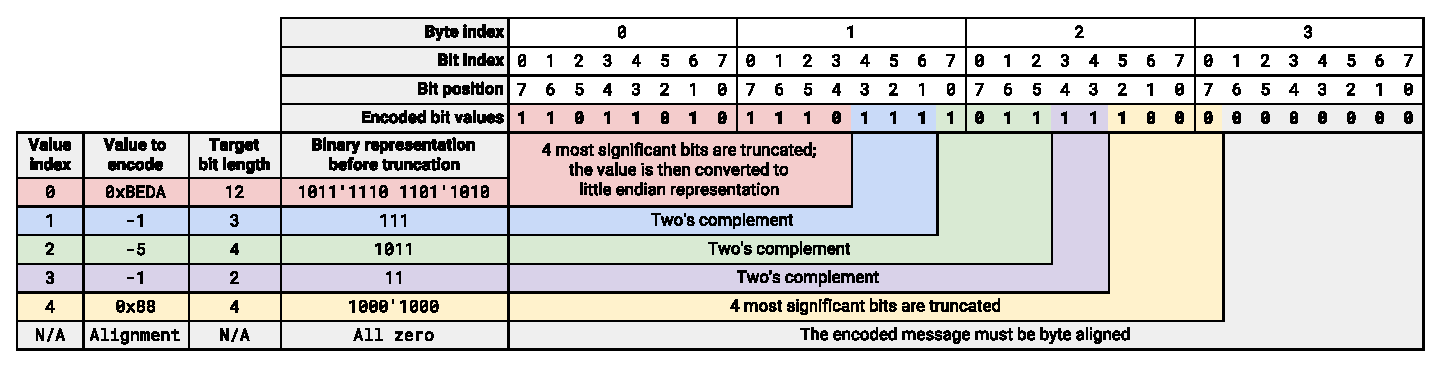
\includegraphics[width=\textwidth]{dsdl/bit-encoding}
	\caption{DSDL serialization example.\label{fig:dsdl_serialization_example}}
\end{figure}

\subsection{Scalar values}

The table \ref{table:dsdl_scalar_serialization} lists the scalar value serialization rules.

\begin{UAVCANSimpleTable}{Scalar value serialization}{|l l X|}\label{table:dsdl_scalar_serialization}
    Type                    & Bit length    & Binary format \\
    \texttt{bool}           & 1
                            & Single bit
                            \\
    \texttt{int\textbf{X}}  & X
                            & Two's complement signed integer
                            \\
    \texttt{uint\textbf{X}} & X
                            & Plain bits
                            \\
    \texttt{float16}        & 16
                            & IEEE 754 binary16
                            \\
    \texttt{float32}        & 32
                            & IEEE 754 binary32
                            \\
    \texttt{float64}        & 64
                            & IEEE 754 binary64
                            \\
    \texttt{void\textbf{X}} & X
                            & X zero bits; ignore when decoding
                            \\
\end{UAVCANSimpleTable}

\subsection{Nested data structures}

Nested data structures are serialized directly in-place,
as if their DSDL definition was pasted directly in place of their reference.
No additional prefixes, suffixes, or padding is provided.

\subsection{Fixed size arrays}

Fixed-size arrays are serialized as a plain sequence of items,
with each item serialized independently in place, with no alignment.
No extra data is added.

Essentially, a fixed-size array of size $X$ elements will be serialized exactly in the same way
as a sequence of $X$ fields of the same type in a row.
Hence, the following two data type definitions will have identical binary representation,
the only actual difference being their representation for the application
if automatic code generation is used.

\begin{minted}{python}
AnyType[3] array
\end{minted}

\begin{minted}{python}
AnyType item_0
AnyType item_1
AnyType item_2
\end{minted}

\subsection{Dynamic arrays}

The following two array definitions are equivalent;
the difference is their representation in the DSDL definition for better readability:
\begin{minted}{python}
AnyType[<42] a      # Can contain from 0 to 41 elements
AnyType[<=41] b     # Can contain from 0 to 41 elements
\end{minted}

A dynamic array is serialized as a sequence of serialized items prepended with an unsigned
integer field representing the number of contained items - the \emph{length field}.
The bit width of the length field is a function of the maximum number of items in the array:
$$\lceil{}\log_2 (X + 1)\rceil{}$$
where $X$ is the maximum number of items in the array.
For example, if the maximum number of items is 251, the length field bit width must be 8 bits;
if the maximum number of items is 1, the length field bit width will be just a single bit.

It is recommended to manually align dynamic arrays by prepending them with void fields
so that the first element is byte-aligned, as that enables more efficient serialization and
deserialization.
This recommendation does not need to be followed if the size of the array elements is not
a multiple of eight bits or if the array elements are of variable size themselves
(e.g., a dynamic array of nested types which contain dynamic arrays themselves).

Consider the following definition:

\begin{minted}{python}
void2                       # Padding - not required, provided as an example
AnyType[<42] array          # The length field is 6 bits wide (see the formula)
\end{minted}

If the array contained three elements,
the resulting binary representation would be equivalent to that of the following definition:

\begin{minted}{python}
void2                       # Padding - not required, provided as an example
uint6 array_length          # Set to 3, because the array contains three elements
AnyType item_0
AnyType item_1
AnyType item_2
\end{minted}

\subsection{Unions}

Similar to dynamic arrays, tagged unions are serialized as two subsequent entities:
the union tag followed by the selected field, with no additional data.

The union tag is an unsigned integer, the bit length of which is a function of the number of fields in the union:
$$\lceil{}\log_2 N\rceil{}$$
where N is the number of fields in the union.
The value serialized in the union tag is the index of the selected field.
Field indexes are assigned according to the order in which they are defined in DSDL,
starting from zero;
i.e. the first defined field has the index 0, the second defined field has the index 1, and so on.

Constants are not affected by the union tag.

It is recommended to manually align unions when they are nested into outer data types by
prepending them with void fields so that the elements are byte-aligned,
as that enables more efficient serialization and deserialization.

Consider the following example:

\begin{minted}{python}
@union                  # In this case, the union tag requires 2 bits
uint16  FOO = 42        # A regular constant attribute
uint16  a               # Index 0
uint8   b               # Index 1
float64 c               # Index 2
uint32  BAR = 42        # Another regular constant
\end{minted}

In order to encode the field \verb|b|, which, according to the definition,
has the data type \verb|uint8|, the union tag should be assigned the value 1.
The following structure will have an identical layout:

\begin{minted}{python}
uint2 tag               # Set to 1
uint8 b                 # The actual data
\end{minted}

If the value of \verb|b| was 7, the resulting serialized byte sequence would be (in binary):
$$%
\underbrace{\texttt{01}}_{\text{tag}}%
\overbrace{\texttt{000001 11}}^{\text{field }\texttt{b}}%
\underbrace{\texttt{000000}}_{\text{padding}}%
$$

\section{Data type compatibility and versioning}\label{sec:dsdl_versioning}

\subsection{Rationale}

As can be seen from the preceding sections,
the concept of \emph{data type} is a cornerstone feature of UAVCAN,
which sets it apart from many competing solutions.

In order to be able to interoperate successfully,
all nodes connected to the same bus must use compatible definitions of all employed data types.
This section is dedicated to the concepts of \emph{data type compatibility}
and \emph{data type versioning}.

A \emph{data type} is a named set of data structures defined in DSDL.
As has been explained above, in the case of message data types,
the set consists of just one data structure, whereas in the case of service data types
the set is a pair of request and response data structures.

Data type definitions may evolve over time as they are refined to better address the needs of their applications.
In order to formalize the data type evolution process with respect to the data type compatibility concerns,
UAVCAN introduces two concepts: \emph{bit compatibility} and \emph{semantic compatibility},
which are discussed below.

\subsection{Bit compatibility}

\subsubsection{Definition}

For the purposes of the definition that follows, a \emph{valid
serialized\footnote{The serialization rules are reviewed in detail in the section \ref{sec:dsdl_data_serialization}.}
representation} of a data structure $A$ is a bit sequence that satisfies the \emph{serialization constraints} of $A$.

\emph{Serialization constraints} limit the set of valid bit sequences according to the data type definition.
A bit sequence meets the serialization constraints if all of the following conditions are
satisfied\footnote{Observe that serialization constraints are not affected by void-typed fields,
because per the serialization rules, the values of void-typed fields are to be set to zero during serialization
and to be ignored during deserialization.}:
\begin{itemize}
    \item Each dynamic array length field contains a valid value;
    i.e. the value of the length field is less than the maximum number of values in the array.

    \item Each union tag field contains a valid value;
    i.e. the value of the tag field is less than the number of alternatives in the union.

    \item The bit sequence is sufficiently long.
\end{itemize}

A data type definition $A$ is bit-compatible with a data type definition $B$ if and only if
the set of valid serialized representations of $A$ is a superset of that of $B$.

$A$ and $B$ are said to be \emph{mutually compatible} if
$A$ is compatible with $B$ and $B$ is compatible with $A$.

\subsubsection{Example}

A \emph{fixed-size data structure} is a structure that does not contain dynamic arrays,
unions, or other structures that contain dynamic arrays or unions within themselves.
As such, the bit length of an serialized representation of a fixed-size structure is constant,
regardless of the data contained in the structure.
Conversely, any data structure that is not fixed-size is called a \emph{variable-size data structure}.

It stands to reason that any data structure definition is compatible with itself.
The following two definitions are bit-compatible as well:

\begin{minted}{python}
uint32 a
uint32 b
\end{minted}

\begin{minted}{python}
uint64 c
\end{minted}

It should be observed that bit-compatibility is invariant to the complexity and the level of nesting
of the data structure.
From the above provided definitions follows that two fixed-size data structures are bit-compatible if the
bit lengths of their respective serialized representations are equal.

Consider the following example data type definition; assume that its full data type name is
\verb|demo.Pair|:

\begin{minted}{python}
# demo.Pair
float16 first
float16 second
\end{minted}

Further, let the following be description of the data type \verb|demo.PairVector|:

\begin{minted}{python}
# demo.PairVector
demo.Pair[3] vector
\end{minted}

Then the following two definitions are bit-compatible:

\begin{minted}{python}
demo.PairVector pair_vector
\end{minted}

\begin{minted}{python}
float16 first_0     # pair_vector.vector[0].first
float16 second_0    # pair_vector.vector[0].second
float16 first_1     # pair_vector.vector[1].first
float16 second_1    # pair_vector.vector[1].second
float16 first_2     # pair_vector.vector[2].first
float16 second_2    # pair_vector.vector[2].second
\end{minted}

The latter definition in the example above is a flattened unrolled form of the former definition.
As such, in that particular example, both definitions can be used interchangeably;
data serialized using one definition can still be meaningful if deserialized using the other definition.
However, it is also possible to construct bit-compatible definitions that are not interchangeable:

\begin{minted}{python}
float16 a
float32 b
\end{minted}

\begin{minted}{python}
float32 a
float16 b
\end{minted}

Even though the above definitions are bit-compatible, one cannot be substituted with the other.
The problem of functional equivalency is addressed by the concept of semantic compatibility,
explored in the section \ref{sec:dsdl_semantic_compatibility}.

The examples above were focused on fixed-size structures.
In the case of fixed-size structures, if $A$ is compatible with $B$, the reverse is also true.
This does not hold for variable-size structures.
Consider the following example:

\begin{minted}{python}
uint8[<=10] a
\end{minted}

\begin{minted}{python}
void1           # The maximum array length is twice lower, so the length prefix is one bit shorter.
uint16[<=5] a   # The 1-bit void field is needed to ensure identical bit offset of the array.
\end{minted}

For the first definition, it is evident that since it contains one dynamic array with
11 possible length values\footnote{Which are 0, 1, 2, 3, 4, 5, 6, 7, 8, 9, and 10.},
and the array type is a fixed-size
structure\footnote{Built-in types can be considered a special case of fixed-size data structures.},
there are 11 possible bit length values for the first definition.

Likewise, for the second definition, there are 6 possible bit length values.

Since both arrays have the same bit offset from the beginning of the bit string,
and taking into account the fact that the element sizes differ by an integral factor,
the set of all possible serialized representations of the second definition is a subset of those of
the first definition.
Possible serialized representations are summarized in the table \ref{table:dsdl_variable_size_compat},
where the columns labeled "First definition" and "Second definition" contain the number of elements in the
respective arrays.

\begin{minipage}{0.7\textwidth}
\begin{UAVCANSimpleTable}{Variable-size data type compatibility example}{|lll|}\label{table:dsdl_variable_size_compat}
    Bit length  & First definition  & Second definition \\
    4           & 0                 & 0 \\
    12          & 1                 & \emph{invalid} \\
    20          & 2                 & 1 \\
    28          & 3                 & \emph{invalid} \\
    36          & 4                 & 2 \\
    44          & 5                 & \emph{invalid} \\
    52          & 6                 & 3 \\
    60          & 7                 & \emph{invalid} \\
    68          & 8                 & 4 \\
    76          & 9                 & \emph{invalid} \\
    84          & 10                & 5 \\
\end{UAVCANSimpleTable}
\end{minipage}

The table illustrates the fact that the first definition is compatible with the second definition,
but the reverse is not true.

Complicated scenarios are possible when a bit belonging to a scalar field is handed over to a
constrained field such as an array length field or a union tag field.
Some interesting examples are shown in the table \ref{table:dsdl_many_compat},
together with a set of valid serialized representation patterns.
Remember that the bits belonging to void-typed fields are ignored during deserialization.

% Please do not remove the hard placement specifier [H], it is needed to keep tables ordered.
\begin{table}[H]\caption{Complex bit compatibility examples}\label{table:dsdl_many_compat}
\begin{tabu}{|l|X|X|X|X|X|}
\hline
\rowfont{\bfseries}
&A                   &   B                 &   C                 &   D                 &   E                 \\
\hline

\multirow{2}{*}{\textbf{Definition}}
&\texttt{void1}      & \texttt{bool x}     & \texttt{void1}      & \texttt{bool x}     & \texttt{bool[<5] a} \\
&\texttt{bool[<3] a} & \texttt{bool[<3] a} & \texttt{bool[<4] a} & \texttt{bool[<4] a} &                     \\
\hline

\multirow{8}{*}{\begin{tabular}[x]{@{}l@{}}\textbf{Valid}\\\textbf{serialized}\\\textbf{representations}\\\end{tabular}}
&\multicolumn{2}{l|}{\texttt{000   }}      & \multicolumn{2}{l|}{\texttt{000    }}     & \texttt{000     } \\
&\multicolumn{2}{l|}{\texttt{001a  }}      & \multicolumn{2}{l|}{\texttt{001a   }}     & \texttt{001a    } \\
&\multicolumn{2}{l|}{\texttt{010aa }}      & \multicolumn{2}{l|}{\texttt{010aa  }}     & \texttt{010aa   } \\
&\multicolumn{2}{l|}{\texttt{      }}      & \multicolumn{2}{l|}{\texttt{011aaa }}     & \texttt{011aaa  } \\
&\multicolumn{2}{l|}{\texttt{100   }}      & \multicolumn{2}{l|}{\texttt{100    }}     & \texttt{100aaaa } \\
&\multicolumn{2}{l|}{\texttt{101a  }}      & \multicolumn{2}{l|}{\texttt{101a   }}     & \texttt{        } \\
&\multicolumn{2}{l|}{\texttt{110aa }}      & \multicolumn{2}{l|}{\texttt{110aa  }}     & \texttt{        } \\
&\multicolumn{2}{l|}{\texttt{      }}      & \multicolumn{2}{l|}{\texttt{111aaa }}     & \texttt{        } \\
\hline

\textbf{Compatible with}
&B                   & A                   & A, B, D             & A, B, C             & \emph{(none)}     \\
\hline
\end{tabu}
\end{table}

\subsection{Semantic compatibility}\label{sec:dsdl_semantic_compatibility}

\subsubsection{Definition}

A data structure definition $A$ is semantically compatible with a data structure definition $B$
if an application that correctly uses $A$ exhibits a functionally equivalent behavior to an application
that correctly uses $B$.
The property of semantic compatibility is commutative.

\subsubsection{Example}

Despite using different binary layouts, the following two definitions are semantically compatible
and also bit-compatible:

\begin{minted}{python}
uint16 FLAG_A = 1
uint16 FLAG_B = 256
uint16 flags
\end{minted}

\begin{minted}{python}
uint8 FLAG_A = 1
uint8 FLAG_B = 1
uint8 flags_a
uint8 flags_b
\end{minted}

Therefore, the definitions can be used
interchangeably\footnote{It should be noted here that due to different set of fields and constants,
the source code auto-generated from the provided definitions may be not drop-in replaceable,
requiring changes in the application. However, application compatibility is orthogonal to
data type compatibility.}.

\subsection{Data type versioning}

\subsubsection{Versioning principles}

Every data type definition has a pair of version numbers -
a major version number and a minor version number, following the principles of semantic versioning.

For the purposes of the following definitions, a \emph{release} of a data type definition stands for
the disclosure of the data type definition to the intended users or to the public,
or for the commencement of usage of the data type definition in a production system.

In order to ensure a deterministic application behavior and ensure a robust migration path
as data type definitions evolve, UAVCAN requires that all data type definitions that share the same
major version number greater than zero must be semantically compatible with each other
and mutually bit-compatible with each other.

Observe that the data type name or its ID do not affect its compatibility.
Regardless, the default data type ID and/or the name of a data type should not be changed after its release,
as that would essentially construe the release of a new data type.

In order to ensure predictable and repeatable behavior of applications that leverage UAVCAN,
the standard requires that once a data type definition is released, it cannot undergo any modifications to
its attributes or directives anymore.
Essentially, released data type definitions are to be considered immutable excepting
comments and whitespace formatting.

Therefore, substantial modifications of released data types are only possible by releasing
new definitions of the same data type.
If it is desired and possible to keep the same major version number for a new definition of the data type,
the minor version number of the new definition shall be one greater than the newest existing minor version
number before the new definition is introduced.
Otherwise, the major version number shall be incremented by one and the minor version shall be set to zero.

An exception to the above rules applies when the major version number is zero.
Data type definitions bearing the major version number of zero are not subjected to any compatibility requirements.
Released data type definitions with the major version number of zero are permitted to change in arbitrary
ways without any regard for compatibility.
It is recommended, however, to follow the principles of immutability, releasing every subsequent definition
with the minor version number one greater than the newest existing definition.

\subsubsection{Major version release constraints}

The DSDL specification limits the number of coexisting major data type versions
in order to simplify support of the data type versioning system at the transport layer
and simplify the management of legacy data type definitions.
As such, at any given moment, the difference between the highest released major version number
and the lowest released major version number of any given data type must not exceed 3.

For example, the following set of released data type definition versions is valid and permissible:
\{0.1, 0.2, 0.3, 1.0, 1.1, 2.0, 2.1, 2.2, 3.0\},
because the difference between the newest released major version (3) and the oldest released major version (0)
does not exceed 3.
The set of the minor versions is not subjected to any constraints,
and as such, there are no limits on the set of concurrently released minor versions.

Continuing with the above example, if it were necessary to release a newer data type definition
under a new major version of 4, the oldest major version of 0 would have to be removed first.
Otherwise, the maximum major version number difference constraint would be violated.
Observe that the actual number of published major versions is irrelevant;
the constraint only applies to the difference between the highest and the lowest released major versions.
For example, shall the version 2 be deprecated and removed while the versions 0 and 1 were still around,
the requirement to remove the version 0 before publishing the version 4 would still hold.
The resulting set of versions may then look like this:
\{1.0, 1.1, 3.0, 4.0\}.

If the difference between the highest and the lowest available major version numbers exceeds 2,
the DSDL compiler must assume that the oldest available definition is marked with an implicit
\verb|@deprecated| directive (section \ref{sec:dsdl_directives}),
even if it is not explicitly provided in the definition.

If the difference between the highest and the lowest available major version numbers exceeds 3,
the DSDL compiler must refuse to process the data type and abort with an error.

\subsubsection{Data type version selection}

There are two aspects to the problem of data type version selection:
compile-time behavior and runtime behavior.
They are explored in this section.

As far as compile-time data type version selection is concerned,
the DSDL compiler is required to compile every available major data type version separately,
allowing the application to choose any available major version at runtime.
However, there may be more than one minor version available per major version;
the DSDL compiler must resolve this ambiguity by always selecting the newest available minor
version per major version at the time of compilation.

For example, consider the following set of data type definition versions:
\{0.1, 0.2, 0.3, 1.0, 1.1, 2.0, 2.1, 2.2, 3.0\}.
As there are four different major data type versions (0, 1, 2, and 3),
the DSDL compiler will make four independent definitions available for the application.
Following the principle of choosing the newest available minor version,
the resulting set of definitions available at runtime will be as follows:
\{0.3, 1.1, 2.2, 3.0\}.

Seeing as the minor version ambiguity is resolved statically,
this information becomes irrelevant for the protocol at runtime.
While implementations can keep the minor version information for diagnostic purposes,
it is completely unnecessary at the transport layer.
As such, the transport layer (which is specified in the chapter \ref{sec:transport_layer})
does not concern itself with the minor data type version information,
whereas the major data type version is attached to every transfer.

The implication is that upon reception of a transfer, the node will use the appropriate
data type definition according to the major data type version information attached to the
transfer; whereas the minor versions used by the emitter and the receiver may mismatch.
The possibility of a minor version mismatch is acceptable because, by definition,
all data type definitions sharing the same major version number are mutually semantically compatible.

When initiating a data exchange (e.g. broadcasting a message or invoking a service),
the node is free to choose the major data type version freely, according to its own application logic.
Nodes that provide services (i.e., servers) must respond to requests using the same major service data type
version that was used in the request.
Again, the minor version number may mismatch, but by the compatibility requirement this is acceptable.

\subsubsection{Versioning example}

Suppose a vendor named \emph{Sirius Cybernetics Corporation} was contracted to design a
cryopod management data bus for a colonial spaceship \emph{Golgafrincham B-Ark}.
Having consulted with applicable specifications and standards, an engineer came up with the following
definition of a cryopod status message type (named \verb|sirius_cyber_corp.golgafrincham_b_ark.cryopod.Status|):

\begin{minted}{python}
# sirius_cyber_corp.golgafrincham_b_ark.cryopod.Status.0.1

float16 internal_temperature    # [kelvin]
float16 coolant_temperature     # [kelvin]

# Status flags in the low byte
uint16 FLAG_COOLING_SYSTEM_A_ACTIVE = 1
uint16 FLAG_COOLING_SYSTEM_B_ACTIVE = 2
# Error flags in the high byte
uint16 FLAG_PSU_MALFUNCTION = 8192
uint16 FLAG_OVERHEATING     = 16384
uint16 FLAG_CRYOBOX_BREACH  = 32768
# Storage for the above defined flags
uint16 flags
\end{minted}

The definition has been deployed to the first prototype for initial lab tests.
Since the definition was experimental, the major version number was set to zero, to signify the
tentative nature of the definition.
Suppose that upon completion of the first trials it was identified that the units must track their power consumption
in real time, for each of the three redundant power supplies independently.
The definition has been amended appropriately.

It is easy to see that the amended definition shown below is neither semantically compatible nor bit-compatible
with the original definition; however, it shares the same major version number of zero, because the backward
compatibility rules do not apply to zero-versioned data types to allow for low-overhead experimentation
before the system is fully deployed and fielded.

\begin{minted}{python}
# sirius_cyber_corp.golgafrincham_b_ark.cryopod.Status.0.2

truncated float16 internal_temperature    # [kelvin]
truncated float16 coolant_temperature     # [kelvin]

saturated float32 power_consumption_0     # Power consumption by the redundant PSU 0 [watt]
saturated float32 power_consumption_1     # likewise for PSU 1
saturated float32 power_consumption_2     # likewise for PSU 2

# Status flags in the low byte
uint16 FLAG_COOLING_SYSTEM_A_ACTIVE = 1
uint16 FLAG_COOLING_SYSTEM_B_ACTIVE = 2
# Error flags in the high byte
uint16 FLAG_PSU_MALFUNCTION = 8192
uint16 FLAG_OVERHEATING     = 16384
uint16 FLAG_CRYOBOX_BREACH  = 32768
# Storage for the above defined flags
uint16 flags
\end{minted}

The last definition was deemed sufficient and deployed to the production system
under the version number of 1.0: \verb|sirius_cyber_corp.golgafrincham_b_ark.cryopod.Status.1.0|.

Having collected empirical data from the fielded systems, the Sirius Cybernetics Corporation has
identified a shortcoming in the v1.0 definition, which was corrected in an updated definition.
Since the updated definition, which is shown below, is mutually semantically
compatible\footnote{The topic of data serialization is explored in detail in the section
\ref{sec:dsdl_data_serialization}.}
with v1.0, the major version number was kept the same and the minor version number was incremented by one:

\begin{minted}{python}
# sirius_cyber_corp.golgafrincham_b_ark.cryopod.Status.1.1

saturated float16 internal_temperature    # [kelvin]
saturated float16 coolant_temperature     # [kelvin]

saturated float32[3] power_consumption    # Power consumption by the PSU

# Status flags
uint8 STATUS_FLAG_COOLING_SYSTEM_A_ACTIVE = 1
uint8 STATUS_FLAG_COOLING_SYSTEM_B_ACTIVE = 2
uint8 status_flags

# Error flags
uint8 ERROR_FLAG_PSU_MALFUNCTION = 5
uint8 ERROR_FLAG_OVERHEATING     = 6
uint8 ERROR_FLAG_CRYOBOX_BREACH  = 7
uint8 error_flags
\end{minted}

Since the definitions v1.0 and v1.1 are mutually semantically compatible,
UAVCAN nodes using either of them can successfully interoperate on the same bus.

Suppose further that at some point a newer version of the cryopod module was released,
with higher precision temperature sensors.
The definition has to be updated accordingly to use \verb|float32| for the temperature fields
instead of \verb|float16|.
Seeing as that change breaks the binary compatibility,
the major version number has to be incremented by one, and the minor version number has to be reset back to zero:

\begin{minted}{python}
# sirius_cyber_corp.golgafrincham_b_ark.cryopod.Status.2.0

float32 internal_temperature    # [kelvin]
float32 coolant_temperature     # [kelvin]

float32[3] power_consumption    # Power consumption by the PSU

# Status flags
uint8 STATUS_FLAG_COOLING_SYSTEM_A_ACTIVE = 1
uint8 STATUS_FLAG_COOLING_SYSTEM_B_ACTIVE = 2
uint8 status_flags

# Error flags
uint8 ERROR_FLAG_PSU_MALFUNCTION = 5
uint8 ERROR_FLAG_OVERHEATING     = 6
uint8 ERROR_FLAG_CRYOBOX_BREACH  = 7
uint8 error_flags
\end{minted}

Now, nodes using v1.0, v1.1, and v2.0 definitions can still coexist on the same network,
but they are not guaranteed to understand each other unless they support all of the used data type definitions.

In practice, nodes that need to maximize their compatibility are likely to employ all existing major versions of
each used data type.
If there are more than one minor versions available, the highest minor version within the major version should
be used, to take advantage of the latest changes in the data type definition.
It is also expected that in certain scenarios some nodes may resort to publishing the same message type
using different major versions concurrently to circumvent compatibility issues (in the
example reviewed here that would be v1.1 and v2.0).

\section{Data type ID}

Whenever a data structure is transferred over the bus, it is accompanied by a non-negative integer
- a \emph{data type ID}.
The data type ID (together with the major version number, which is also exchanged over the bus together with the
data type ID) is used by receiving nodes to determine which data type definition to use
to process the received data structure.
The data type ID value does not affect data type compatibility.

It stands to reason that in order to be able to interoperate successfully,
every node connected to the bus must use identical mapping between data types and their identifiers.

There are two \emph{kinds} of data types: message data types and service data types.
Each kind has an independent set of data type identifiers.
Each kind has a reserved subset which is used for standard data type definitions,
and a dedicated subset for vendor-specific data type definitions.
More info on the reserved subsets is provided in the chapter \ref{sec:application_layer}.
The permitted ranges of data type ID values are specified in the table \ref{table:dsdl_dtid_ranges}.

\begin{UAVCANSimpleTable}{Data type ID ranges per data kind}{|l|c c|X|}\label{table:dsdl_dtid_ranges}
    Kind            & Minimum & Maximum & Note \\

    Message type    & 0       & 65535   & Representable as 16-bit unsigned integer (2 octets).
                                          The range of message data type ID usable with anonymous message
                                          transfers is further limited; more info in the
                                          chapter \ref{sec:transport_layer}. \\

    Service type    & 0       & 255     & Representable as 8-bit unsigned integer (1 octet). \\
\end{UAVCANSimpleTable}

All UAVCAN nodes must use the same data type ID mapping for the standard data types,
as defined by the default data type ID values provided for each of the standard data types.
Since the standard data type ID mapping is immutable, all standard-compliant nodes can always
use standard data types conflict-free.

Vendor-specific data types, however, do not enjoy the lack of conflict guarantee,
because by virtue of being vendor-specific, such data types cannot use a global
fixed agreed upon mapping like the standard data types do.
As such, whenever vendor-specific data types are used, there is always a risk that
different nodes may map different data types to the same data type ID.

It is the responsibility of the system integrator to ensure that if vendor-specific data types are
used, the data type ID mappings are configured on all nodes identically.
Vendors of UAVCAN equipment must provide the integrator with a way to change the data type ID
of any vendor-specific data type leveraged by the node\footnote{Nodes that fail to provide a way of
altering the data type ID mapping for vendor-specific data types cannot be considered standard-compliant.}.

\section{Standard and vendor-specific data types}

\subsection{Standard data type repository}

The DSDL definitions of the standard data types are available in the official DSDL repository,
which is linked from the project homepage at \href{http://uavcan.org}{uavcan.org}.

Information concerning development and maintenance of the standard DSDL definitions is available
in the chapter \ref{sec:introduction}.

\subsection{Vendor-specific data types}

Vendors must define their specific data types in a separate namespace,
which should typically be named to match their company name.
Separation of the vendor's definitions into a dedicated namespace ensures that no name conflicts will occur
in systems that utilize vendor-specific data types from different providers.
Note that, according to the naming requirements, the name of a DSDL namespace must start
with an alphabetic character; therefore, a company whose name starts with a digit will have to resort to
a mangled name, e.g. by moving the digits towards the end of the name,
or by spelling the digits in English (e.g. 42 - \verb|fortytwo|).

Defining vendor-specific data types within the standard namespace (\verb|uavcan.|) is explicitly prohibited.
The standard namespace will always be used only for standard data types.

Generally speaking, it is desirable for "generic" data types to be included into the standard set.
Vendors should strive to design their data types as generic and as independent of their specific use
cases as possible.
The SI system of measurement units should be preferred;
data type definitions that make unnecessary deviations from SI will not be accepted into the standard set.


\chapter{Transport layer}\label{sec:transport_layer}

This chapter defines the transport layer of UAVCAN.
First, general implementation-agnostic concepts are introduced.
Afterwards, they are further defined for each supported transport medium, e.g., CAN FD.

As the specification is extended to add support for new transport protocols,
some of the generic aspects may be pushed to lower-level transport-specific sections
if they are found to map poorly on the newly added transports.
Such changes are guaranteed to preserve full backward compatibility of the existing transport protocols.

\section{Core concepts}

\subsection{Transfer}

A \emph{transfer} is an act of data transmission between nodes.

\subsubsection{Broadcast and unicast transfers}

A transfer that is addressed to any interested node except the source node is a \emph{broadcast transfer}.
A transfer that is addressed to one particular node is a \emph{unicast transfer}.

In the case of broadcast transfers, the sending node makes the data widely available on the bus,
allowing any interested node to freely opt-in and process
it\footnote{The word ``broadcast'' should not lead one to believe that every node is required to
process such transfers. The opt-in logic is facilitated by automatic acceptance filtering features
implemented on the transport layer.}.
The decision of whether to process any given transfer or not is made by receiving nodes.

In the case of unicast transfers, the addressing logic is inverted:
the sending node decides which particular remote node should receive the transfer.
All other nodes remain unaffected by such transmission and take no part in the addressing process.

\subsubsection{Message and service transfers}

A \emph{message transfer} is a broadcast transfer that contains a serialized message and its
metadata\footnote{Such as the subject ID and the source node ID.}.

A \emph{service transfer} is a unicast transfer that contains either a service request or a service response
with related metadata.

\subsubsection{Single-frame and multi-frame transfers}

Both message and service transfers can be further distinguished between single-frame and multi-frame transfers.

A \emph{single-frame transfer} is a transfer that is entirely contained in a single transport frame.
The amount of data that can be exchanged using single-frame transfers is dependent on the transport protocol in use.

A \emph{multi-frame transfer} is a transfer that has its payload distributed over multiple transport frames.
The UAVCAN protocol stack handles transfer decomposition and reassembly automatically.

The choice between single-frame and multi-frame transfers is made by the UAVCAN protocol logic on
the transmitting node based on the amount of payload data to be transferred.
The application does not have any control over the type of transfer that will be used
except limiting the amount of payload data.
UAVCAN protocol implementations must always choose single-frame transfers if possible;
multi-frame transfers can be used only if all of the requested payload cannot be allocated in one transport frame.

\subsubsection{Common properties}

The properties listed in the table \ref{table:common_transfer_properties} are common to all types of transfers.

\begin{UAVCANSimpleTable}{Common transfer properties}{|l X|}\label{table:common_transfer_properties}
    Property        & Description \\
    Payload         & The serialized data structure. \\
    Port ID         & A numerical identifier that indicates how the data should be processed.
                      This is the subject ID for message transfers and service ID for service transfers. \\
    Source node ID  & The node ID of the transmitting node (excepting anonymous message transfers). \\
    Priority        & A non-negative integer value that defines the transfer urgency.
                      Higher priority transfers can preempt lower priority transfers. \\
    Transfer ID     & A small overflowing integer that increments with every transfer
                      of this data type from a given node. \\
\end{UAVCANSimpleTable}

\subsection{Message publication}

Message publication is the main method of communication between UAVCAN nodes.

A published message is carried by a single message transfer that contains the serialized message data structure.
A published message does not contain any additional fields besides those listed in the table
\ref{table:common_transfer_properties}.

In order to publish a message, the publishing node must have a node ID that is unique within the network.
An exception applies to \emph{anonymous message publications}.

\subsubsection{Anonymous message publication}\label{sec:transport_anonymous_message_publication}

An anonymous message transfer is a transfer that can be sent from a node that does not have a node ID.
This kind of message transfer is especially useful for facilitation of \emph{plug-and-play nodes}
(a high-level concept that is reviewed in detail in chapter \ref{sec:application_layer}).

A node that does not have a node ID is said to be in \emph{passive mode}.
Passive nodes are unable to initiate regular data exchanges,
but they can listen to the transfers exchanged over the bus,
and they can emit anonymous message transfers.

An anonymous message has the same properties as a regular message, except for the source node ID.

An anonymous transfer can only be a single-frame transfer. Multi-frame anonymous message transfers are not allowed.
This restriction must be kept in mind when designing message data types
intended for use with anonymous message transfers:
when used with anonymous transfers, the whole message must fit into a single transport frame;
however, the same data type can be used with multi-frame regular (non-anonymous) transfers, if desired.

The set of message subject ID values that can be used with anonymous messages may be limited
depending on the transport protocol in use\footnote{This is considered to be an acceptable limitation because
anonymous transfers are intended for an extremely limited set of use cases.}.
It is guaranteed, however, that the subject ID values in the range
from 65528 ($\text{FFF8}_\text{16}$) to 65535 ($\text{FFFF}_\text{16}$), inclusively,
are always available for use with anonymous messages regardless of the transport in use.

Anonymous messages may require special handling logic depending on the transport layer in use.

\subsubsection{Message timing requirements}

Generally, a message transmission should be aborted if it cannot be completed in 1 second.
Applications are allowed to deviate from this recommendation,
provided that every such deviation is explicitly documented.
It is expected that high-frequency high-priority messages may opt for lower timeout values,
whereas low-priority delayable data may opt for higher timeout values to account for network congestion.

\subsection{Service invocation}

A service invocation sequence consists of two related service transfers:
\emph{service request transfer} and \emph{service response transfer}.

A service request transfer is sent from the invoking node -- \emph{client node} -- to the node
that provides the service -- \emph{server node}.
Upon handling the request, the server node responds to the client node with a service response transfer.
The client will match the response with the corresponding request by comparing the following values:
server node ID, service ID, and the transfer ID.

The tables \ref{table:service_request_transfer_properties} and \ref{table:service_response_transfer_properties}
describe the properties of service request and service response transfers, respectively.

Both the client and the server must have node ID values that are unique within the network;
service invocation is not available to passive nodes.
The client and the server must be two distinct nodes.

\begin{UAVCANSimpleTable}{Service request transfer properties}{|l X|}\label{table:service_request_transfer_properties}
    Property                        & Description \\
    Payload                         & The serialized service request data structure. \\
    Service ID                      & See the table \ref{table:common_transfer_properties}. \\
    Source node ID                  & The node ID of the client (the invoking node). \\
    Destination node ID             & The node ID of the server (the invoked node). \\
    Priority                        & See the table \ref{table:common_transfer_properties}. \\
    Transfer ID                     & An integer value that:
        \begin{enumerate}
            \item allows the server to distinguish the request from other requests from the same client;
            \item allows the client to match the response with its request.
        \end{enumerate} \\
\end{UAVCANSimpleTable}

\begin{UAVCANSimpleTable}{Service response transfer properties}{|l X|}\label{table:service_response_transfer_properties}
    Property                        & Description \\
    Payload                         & The serialized service response data structure. \\
    Service ID                      & Same value as in the request transfer. \\
    Source node ID                  & The node ID of the server (the invoked node). \\
    Destination node ID             & The node ID of the client (the invoking node). \\
    Priority                        & Same value as in the request transfer. \\
    Transfer ID                     & Same value as in the request transfer. \\
\end{UAVCANSimpleTable}

\subsubsection{Service timing requirements}

Applications are recommended to follow the service invocation timing recommendations specified below.
Applications are allowed to deviate from these recommendations,
provided that every such deviation is explicitly documented.

\begin{itemize}
    \item Service transfer transmission should be aborted if does not complete in 1 second.
    \item The client should stop waiting for a response from the server if one has not arrived within 1 second.
\end{itemize}

If the server uses a significant part of the timeout period to process the request,
the client might drop the request before receiving the response.
It is recommended to ensure that the server will be able to process any request in less than 0.5 seconds.

\subsection{Transfer priority}\label{sec:transfer_prioritization}

UAVCAN transfers are prioritized by means of the transfer priority property,
which allows at least 8 (eight) different priority levels for all types of transfers
(some transports may support more than eight priority levels).
Transfers with higher priority levels preempt transfers with lower priority levels,
delaying their transmission until there are no more higher priority transfers to exchange.

\begin{remark}[breakable]
    The priority level mnemonics and their usage recommendations are specified in the following list.
    The mapping between the mnemonics and actual numeric identifiers is transport-dependent.

    % https://forum.uavcan.org/t/transfer-priority-level-mnemonics/218/6?u=pavel.kirienko
    \begin{description}
        \item[Exceptional] -- The bus designer can ignore these messages when calculating bus load since they
        should only be sent when a total system failure has occurred.
        For example, a self-destruct message on a rocket would use this priority.
        Another analogy is an NMI on a microcontroller.

        \item[Immediate] -- Immediate is a ``high priority message'' but with additional latency constraints.
        Since exceptional messages are not considered when designing a bus, the latency of immediate messages
        can be determined by considering only immediate messages.

        \item[Fast] -- Fast and immediate are both ``high priority messages'' but with additional latency constraints.
        Since exceptional messages are not considered when designing a bus,
        the latency of fast messages can be determined by considering only immediate and fast messages.

        \item[High] -- High priority messages are more important than nominal messages but have looser
        latency requirements than fast messages. This priority is used so that,
        in the presence of rogue nominal messages, important commands can be received.
        For example, one might envision a failure mode where a temperature sensor starts to
        load a vehicle bus with nominal messages.
        The vehicle remains operational (for a time) because the controller is exchanging fast and
        immediate messages with sensors and actuators.
        A system safety monitor is able to detect the distressed bus and command the vehicle to a
        safe state by sending high priority messages to the controller.

        \item[Nominal] -- This is what all messages should use by default.
        Specifically the heartbeat messages should use this priority.

        \item[Low] -- Low priority messages are expected to be sent on a bus under all conditions but cannot
        prevent the delivery of nominal messages.
        They are allowed to be delayed but latency should be constrained by the bus designer.

        \item[Slow] -- Slow messages are low priority messages that have no time sensitivity at all.
        The bus designer need only ensure that, for all possible system states,
        these messages will eventually be sent.

        \item[Optional] -- These messages might never be sent (theoretically) for some possible system states.
        The system must tolerate never exchanging optional messages in every possible state.
        The bus designer can ignore these messages when calculating bus load.
        This should be the priority used for diagnostic or debug messages that are not required on an
        operational system.
    \end{description}
\end{remark}

\subsection{Transfer descriptor}\label{sec:transfer_descriptor}

Transfer emission and reception processes rely on the concept of \emph{transfer descriptor}.

A transfer descriptor is a set of properties that identify a particular set of transfers that originate
from the same source node, share the same port ID, same kind (message or service), and are addressed to the same
destination node (the latter applies only to unicast transfers).

The properties that constitute a transfer descriptor are listed below:

\begin{itemize}
    \item Transfer kind (message or service).
    \item Port ID (subject ID for message transfers, service ID for service transfers).
    \item Source node ID.
    \item Destination node ID (only for service transfers).
\end{itemize}

For convenience, two derived definitions are introduced.
Their objective is to simplify the description of transfer reception and emission logic that appears later in this
specification.
\begin{description}
    \item[Emitted transfer descriptor] -- a transfer descriptor where the source node ID equals the local node's ID.
    \item[Received transfer descriptor] -- a transfer descriptor where the destination node ID equals
    the local node's ID (for service transfers) or is not defined (for message transfers).
\end{description}

\subsubsection{Hard real-time considerations}

Hard real-time applications require a predictable and deterministic data processing time.
The concept of transfer descriptor plays an important role in communication;
hence, its contribution to the worst case data processing load should be carefully analyzed.

\begin{remark}
    From the above definition of transfer descriptor it is easy to derive that for any
    message subject ID or any service subject ID the maximum number of transfer descriptors
    that can be observed by the local node will never exceed the number of nodes on the bus minus
    one\footnote{The local node cannot exchange data with itself, hence minus one.}.
    If the number of nodes on the bus cannot be known in advance, it can be considered to equal 128,
    which is the maximum node capacity of a UAVCAN bus.

    The total number of distinct transfer descriptors that can be observed by a node on any valid UAVCAN bus
    is a product of the number of distinct port ID values utilized by the node and the number of other nodes on the bus.

    The transport emission and reception logic defined later in this specification relies on data structures
    indexed by transfer descriptor values.
    Elements of such structures can be easily accessed via constant-complexity static look-up tables
    because the worst case number of elements is always statically known.
\end{remark}

\section{Transfer emission}

\subsection{Transfer ID computation}\label{sec:transfer_id}

The \emph{transfer ID} is a small unsigned integer value in the range from 0 to 31, inclusive,
that is provided for every transfer.
This value is crucial for many aspects of UAVCAN communication\footnote{One might be tempted to use the transfer ID
value for temporal synchronization of parallel message streams originating from the same node,
where messages bearing the same transfer ID value are supposed to correspond to the same moment of time.
Such use is strongly discouraged because it is impossible to detect if one node is more than
32 messages behind another.
If temporal synchronization is necessary, explicit time stamping should be used instead.};
specifically:
\begin{description}
    \item[Message sequence monitoring] - the continuously increasing transfer ID allows receiving nodes to
    detect lost messages and detect when a message stream from any remote node is interrupted.

    \item[Service response matching] - when a server responds to a request, it uses the same transfer ID for the
    response as in the request,
    allowing any node to emit concurrent requests to the same server while being able to
    match each response with the corresponding request.

    \item[Transport frame deduplication] - for single-frame transfers,
    the transfer ID allows receiving nodes to work around the transport
    frame duplication problem\footnote{This is a well-known issue that can be observed with certain
    transports such as CAN bus -- a frame that appears valid to the receiver may under certain
    (rare) conditions appear invalid to the transmitter, triggering the latter to retransmit the frame,
    in which case it will be duplicated on the side of the receiver.
    Sequence counting mechanisms such as the transfer ID or the toggle bit (both of which are used in UAVCAN)
    allow applications to circumvent this problem.} (multi-frame transfers combat the frame duplication
    problem using the toggle bit, which is introduced later).

    \item[Multi-frame transfer reassembly] - more info is provided in section \ref{sec:transfer_reception}.

    \item[Automatic management of redundant interfaces] - the transfer ID parameter allows the UAVCAN protocol
    stack to perform automatic switchover to a back-up interface shall the primary interface fail.
    The switchover logic can be completely transparent to the application, joining several independent
    redundant physical transports into a highly reliable single virtual communication channel.
\end{description}

For message transfers and service request transfers the ID value should be computed as described below.
For service response transfers this value must be directly copied from the corresponding service request transfer.

Every node that is interested in emitting transfers must maintain a mapping
(or a similar functionally equivalent static structure\footnote{For example, simple static variables.})
from emitted transfer descriptors (section \ref{sec:transfer_descriptor}) to transfer ID counters.
This mapping is referred to as the \emph{emitted transfer ID map}.

Whenever a node needs to emit a transfer, it will query its transfer ID map for the appropriate transfer descriptor.
If the map does not contain such entry, a new entry will be created with the transfer ID counter initialized to zero.
The node will use the current value of the transfer ID from the map for the transfer,
and then the value stored in the map will be incremented by one.
When the stored transfer ID exceeds its maximum value, it will roll over to zero.

It is expected that some nodes will need to emit certain transfers aperiodically or on an ad-hoc basis,
thereby creating unused entries in the emitted transfer ID map.
If such aperiodic or ad-hoc transfers are of interest,
the worst case number of unused entries can be determined statically as a function of the number of
port identifiers used and the number of addressed nodes on the bus (the latter applies to services only).
Nodes are not allowed to remove any entries from the transfer ID map as long as they are running.

\subsection{Single frame transfers}

If the size of the entire transfer payload does not exceed the space available for payload in a single transport frame,
the whole transfer will be contained in one transport frame.
Such transfer is called a \emph{single-frame transfer}.

Single frame transfers are more efficient than multi-frame transfers in terms of throughput, latency,
and data overhead.

\subsection{Multi-frame transfers}\label{sec:transport_multi_frame_transfers}

\emph{Multi-frame transfers} are used when the size of the transfer payload exceeds the space available
for payload in a single transport frame.

Two new concepts are introduced in the context of multi-frame transfers, both of which are reviewed below in detail:
\begin{samepage}
\begin{itemize}
    \item Transfer CRC\footnote{CRC stands for ``cyclic redundancy check'', an error-detecting code
    added to data transmissions to reduce the likelihood of undetected data corruption.}.
    \item Toggle bit.
\end{itemize}
\end{samepage}

In order to emit a multi-frame transfer, the node must first compute the CRC for the entirety of the transfer payload.
The node appends the resulting CRC value at the end of the transfer payload in the big-endian byte order,
and then emits the resulting byte set in chunks as an ordered sequence of transport frames,
where the first transport frame contains the beginning of the payload bytes,
and the last transport frame contains the last bytes of the payload (possibly none) plus the transfer CRC.

The data field of all transport frames of a multi-frame transfer, except the last one, should be fully utilized.
Applications are allowed to limit the maximum amount of data transferred per transport frame in order to
improve the preemption granularity, thus reducing the worst case latency of higher priority
transfers\footnote{For example, some CAN FD applications may choose to restrict the maximum payload size to 32 bytes
rather than the protocol limit of 64 bytes, as that provides more opportunities for higher-priority frames to
take over the bus. The trade-off is that smaller frames lead to higher transfer fragmentation, increase the bus load,
and increase the overall average latency.}.
Receiving nodes must be prepared to reconstruct multi-frame transfers that utilize the
available payload space partially.

All frames of a multi-frame transfer should be pushed to the transmission queue at once,
in the proper order from the first frame to the last frame.
Explicit gap time between transport frames belonging to the same transfer should not be introduced;
rather, implementations always should strive to minimize it.
Re-ordering of frames belonging to the same multi-frame transfer is prohibited.

\subsubsection{Transfer CRC}\label{sec:transfer_crc}

Transfer CRC allows receiving nodes to ensure that a received multi-frame transfer has been reassembled correctly.

It should be understood that the transfer CRC is not intended for bit-level data integrity checks,
as that must be managed by the transport layer implementation on a per-frame
basis\footnote{Bit-level errors at the transport frame level may compromise the error-detecting
properties of the transfer CRC.}.
As such, the transfer CRC allows receiving nodes to ensure that all of the frames of a multi-frame
transfer were received, all of the received frames were reassembled in the correct order,
and that all of the received frames belong to the same multi-frame transfer.

The transfer CRC is computed over the entire payload of the transfer.
Certain transport implementations\footnote{Such as CAN FD.} may require a short sequence of padding bytes
to be added at the end of the transfer payload due to the low granularity of the frame payload length property;
in that case, the padding bytes must be included in the CRC computation as well,
as if they were part of the useful payload.

The resulting CRC value is appended to the transfer in the \emph{big-endian byte order}
(most significant byte first),
in order to take advantage of the CRC residue check intrinsic to the used algorithm.

The transfer CRC algorithm specification is provided in the table \ref{table:transfer_crc_params}.

\begin{minipage}{0.7\textwidth}
\begin{UAVCANSimpleTable}{Transfer CRC algorithm parameters}{|ll|}\label{table:transfer_crc_params}
    Property        & Value \\
    Name            & CRC-16/CCITT-FALSE \\
    Initial value   & \texttt{0xFFFF} \\
    Polynomial      & \texttt{0x1021} \\
    Reverse         & No \\
    Output XOR      & $0$ \\
    Residue         & $0$ \\
    Check           & $\left(49, 50, \ldots, 56, 57\right) \rightarrow \mathtt{0x29B1}$ \\
\end{UAVCANSimpleTable}
\end{minipage}

The following code snippet provides a basic implementation of the transfer CRC algorithm in C++.

\begin{minipage}{0.9\textwidth}
\begin{minted}{cpp}
// UAVCAN transfer CRC algorithm implementation in C++.
// License: CC0, no copyright reserved.

#include <iostream>
#include <cstdint>
#include <cstddef>

class TransferCRC
{
    std::uint16_t value_ = 0xFFFFU;

public:
    void add(std::uint8_t byte)
    {
        value_ ^= static_cast<std::uint16_t>(byte) << 8U;
        for (std::uint8_t bit = 8; bit > 0; --bit)
        {
            if ((value_ & 0x8000U) != 0)
            {
                value_ = (value_ << 1U) ^ 0x1021U;
            }
            else
            {
                value_ = value_ << 1U;
            }
        }
    }

    void add(const std::uint8_t* bytes, std::size_t length)
    {
        while (length-- > 0)
        {
            add(*bytes++);
        }
    }

    [[nodiscard]] std::uint16_t get() const { return value_; }
};

int main()
{
    TransferCRC crc;
    crc.add(reinterpret_cast<const std::uint8_t*>("123456789"), 9);
    std::cout << std::hex << "0x" << crc.get() << std::endl;  // Outputs 0x29B1
    return 0;
}
\end{minted}
\end{minipage}

\subsubsection{Toggle bit}\label{sec:toggle_bit}

The toggle bit is a property defined at the transport frame level.
Its purpose is to detect and avoid transport frame duplication errors in multi-frame
transfers\footnote{In single-frame transfers, transport frame deduplication is based on the transfer ID counter.}.

The toggle bit of the first transport frame of a multi-frame transfer must be set to one.
The toggle bits of the following transport frames of the transfer must alternate,
i.e., the toggle bit of the second transport frame must be zero,
the toggle bit of the third transport frame must be one, and so on.

For single-frame transfers, the toggle bit must be set to one or removed completely,
whichever option works best for the particular transport.

Transfers where the initial value of the toggle bit is zero must be ignored.
The initial state of the toggle bit may be inverted in the future revisions of the protocol
to facilitate automatic protocol version detection.

\subsection{Redundant interface support}

In configurations with redundant bus interfaces,
nodes are required to submit every outgoing transfer to the transmission queues of
all available redundant interfaces simultaneously.
It is recognized that perfectly simultaneous transmission may not be possible due to different
utilization rates of the redundant interfaces and different phasing of their traffic;
however, that is not an issue for UAVCAN.
If perfectly simultaneous frame submission is not possible, interfaces with lower numerical index
should be handled in the first order.

An exception to the above rule applies if the payload of the transfer depends on some properties
of the interface through which the transfer is emitted.
An example of such a special case is the time synchronization algorithm leveraged by UAVCAN
(documented in chapter \ref{sec:application_layer} of the specification).

Redundant interfaces are used for increased fault tolerance, not for load sharing reasons.
Whenever a node is connected to an interface the likelihood of the interface failing is increased.
This suggests that backup interfaces may only interconnect with mission-critical equipment,
unless a homogeneous network architecture is desired\footnote{Heterogeneous transport configuration
complicates the analysis of the network, which might make it impractical in safety-critical deployments.
In that case, a simpler configuration where each available redundant bus is connected to every node may be
preferred.}.
See section \ref{sec:phy_non_uniform_transport_redundancy}.

\section{Transfer reception}\label{sec:transfer_reception}

\subsection{Transfer ID comparison}\label{sec:transfer_id_forward_distance}

The following explanation relies on the concept of the \emph{transfer ID forward distance}.
Transfer ID forward distance $F$ is a function of two transfer ID values,
$A$ and $B$, that defines the number of increment operations that need to be applied to
$A$ so that $A^\prime{} = B$, assuming modulo 32 arithmetic\footnote{%
    For example:
    $A=0, B=0, F\rightarrow0$;
    $A=0, B=5, F\rightarrow5$;
    $A=5, B=0, F\rightarrow27$;
    $A=31, B=30, F\rightarrow31$;
    $A=31, B=0, F\rightarrow1$.
}:
$$A + F = B \quad (\bmod{}\ 32)$$
The \emph{half range} of transfer ID is 16.

The following code sample provides an example implementation of the transfer ID comparison algorithm in C++.

\begin{minipage}{0.9\textwidth}  % Mini page is needed to prevent page breaks within the snippet
\begin{minted}{cpp}
// UAVCAN transfer ID forward distance computation algorithm implemented in C++.
// License: CC0, no copyright reserved.

#include <cstdint>
#include <iostream>
#include <cassert>

constexpr std::uint8_t TransferIDBitLength = 5;  // Defined by the specification

[[nodiscard]]
constexpr std::uint8_t computeForwardDistance(std::uint8_t a, std::uint8_t b)
{
    constexpr std::uint8_t MaxValue = (1U << TransferIDBitLength) - 1U;
    assert((a <= MaxValue) && (b <= MaxValue));

    std::int16_t d = static_cast<std::int16_t>(b) - static_cast<std::int16_t>(a);
    if (d < 0)
    {
        d += 1U << TransferIDBitLength;
    }

    assert(d >= 0);
    assert(d <= MaxValue);
    assert(((a + d) & MaxValue) == b);
    return static_cast<std::uint8_t>(d);
}

int main()
{
    assert(0  == computeForwardDistance(0, 0));
    assert(1  == computeForwardDistance(0, 1));
    assert(7  == computeForwardDistance(0, 7));
    assert(0  == computeForwardDistance(7, 7));
    assert(31 == computeForwardDistance(31, 30)); // overflow
    assert(1  == computeForwardDistance(31, 0));  // overflow
    return 0;
}
\end{minted}
\end{minipage}

\subsection{State variables}

\subsubsection{Main principles}

Nodes that receive transfers must keep a certain set of state variables for each
received transfer descriptor (section \ref{sec:transfer_descriptor}).

The set of state variables as documented in the table \ref{table:transfer_receiver_state_variables}
will be referred to as the \emph{receiver state}.
For the purposes of this specification, it is assumed that the node will maintain a
mapping from transfer descriptors to receiver states, which will be referred to as the \emph{receiver map}.
It is understood that implementations might prefer different architectures, which is permitted as
long as the resulting behavior of the node observable at the protocol level is functionally equivalent.

Whenever a node receives a transfer, it will query its receiver map for the matching received transfer descriptor.
If the matching state does not exist, the node will add a new receiver state to the map
and initialize it as defined in section \ref{sec:transfer_reception_initial_state}.
The node then will proceed with the procedure of \emph{receiver state update},
which is defined in section \ref{sec:transfer_reception_state_update_redundant} for redundant transports
and section \ref{sec:transfer_reception_state_update_non_redundant} for non-redundant transports.

It is expected that some transfers will be aperiodic or ad-hoc,
which implies that the receiver map may over time accumulate receiver states that are no longer used.
Therefore, nodes are allowed, but not required, to remove any receiver state from the receiver map
as soon as the state reaches the \emph{transfer ID timeout condition}\footnote{Such behavior is
not recommended for hard real-time applications, where deterministic static look-up tables
should be preferred instead.},
as defined in section \ref{sec:transfer_id_timeout_condition}.

Receiver state can only be modified when a new transport frame of a matching transfer is received.
This guarantee simplifies implementation, as it implies that the receiver states will not
require any periodic background maintenance activities.

\begin{UAVCANSimpleTable}{Transfer reception state variables}{|l X|}
    State               & Description \label{table:transfer_receiver_state_variables} \\
    Transfer payload    & Useful payload byte sequence; extended upon reception of new matching transport frames. \\
    Transfer ID         & The transfer ID value of the next expected transport frame. Section \ref{sec:transfer_id}. \\
    Next toggle bit     & Expected value of the toggle bit in the next transport frame.
                          Section \ref{sec:toggle_bit}. \\
    Transfer timestamp  & The local monotonic timestamp sampled when the first frame of the transfer arrived.
                          Here, ``monotonic'' means that the reference clock does not change its rate or make leaps. \\
    Interface index     & Only in the case of redundant transport interfaces. \\
\end{UAVCANSimpleTable}

\subsubsection{Initial state}\label{sec:transfer_reception_initial_state}

The initial state is reached when a new entry of the receiver map is created or an existing entry is reset.
Like any other state update, an entry can be created or reset only synchronously with
the reception of a matching transport frame.

Upon reset, the receiver state will meet the following conditions:

\begin{itemize}
    \item The transfer payload buffer is empty.
    \item The transfer ID state matches the actual transfer ID value from the newly received transfer,
    unless this is a non-first frame of a multi-frame transfer.
    In the latter case, the transfer ID state will match the received transfer ID value incremented by one.
    \item The toggle bit is set to its initial state (section \ref{sec:toggle_bit}).
    \item The transfer timestamp matches the reception timestamp from the transport frame.
    \item The interface index matches the index of the interface that the new frame was received from
    (for nodes with redundant interfaces only).
\end{itemize}

A receiver state must be reset when any of the following conditions are met:

\begin{itemize}
    \item A new receiver state instance is created.

    \item A transfer ID timeout condition is reached (section \ref{sec:transfer_id_timeout_condition}).

    \item A first frame of a transfer (either a multi-frame or a single-frame; in the latter case, the same frame
    would also be the last frame of the transfer) is received from the same interface as the previous frame
    (does not apply to non-redundantly interfaced nodes),
    and the transfer ID forward distance (section \ref{sec:transfer_id_forward_distance}) from the received
    transfer ID to the stored transfer ID is greater than one.

    \item Only for redundantly interfaced nodes: A first frame of a transfer is received,
    an interface switchover condition is reached (section \ref{sec:transfer_interface_switchover_condition}),
    and the transfer ID forward distance from the stored transfer ID to the received transfer ID is
    less than the transfer ID half range (section \ref{sec:transfer_id_forward_distance}).
\end{itemize}

\subsubsection{Transfer ID timeout condition}\label{sec:transfer_id_timeout_condition}

A state is said to have reached the transfer ID timeout condition
if the last matching transfer was seen more than 2 (two) seconds ago.
When this condition is reached, the receiver must accept the next transfer disregarding its transfer ID value.

Nodes are allowed to use different timeout values, if that is believed to benefit the application.
If a different timeout value is used, it must be explicitly documented.

Low timeout values increase the risk of undetected transfer duplication when such transfers are significantly
delayed due to bus congestion, which is possible with very low-priority transfers when the bus utilization is high.

High timeout values increase the risk of an undetected transfer loss when a remote node suffers an emitted transfer ID
map state loss (e.g., due to the whole node being restarted).
However, the effects of such a transfer loss caused by a loss of state on a remote node
are always constrained to the first transfer only.

\subsubsection{Interface switchover condition}\label{sec:transfer_interface_switchover_condition}

This condition is only applicable for configurations with redundant transport interfaces.
It means that the node is allowed to receive the next transfer from an interface that is not the same
the previous transfer was received from.

The condition is reached when the last matching transfer was successfully received more than
$T_\text{switch}$ seconds ago. The value of $T_\text{switch}$ should not exceed the reception transfer
ID timeout, as defined in section \ref{sec:transfer_id_timeout_condition},
because if $T_\text{switch}$ were to exceed the transfer ID timeout, an interface switchover would be
performed by the normal receiver state reset procedure, rendering $T_\text{switch}$ useless.

The actual value of $T_\text{switch}$ can be either a constant chosen by the designer according
to the application requirements (e.g., the maximum recovery time in the event of an interface failure),
or the protocol stack can estimate this value automatically by analyzing the transfer intervals.

Nodes are required to let the first interface time out before using the next one because the
transfer ID field is expected to wrap around frequently (every 32 transfers).
Different interfaces are expected to exhibit different latencies even in a properly functioning system,
especially if the system contains both redundantly-interfaced and non-redundantly-interfaced nodes.
If the latency of a backup interface relative to the primary interface exceeds 32 transfer intervals,
and receiving nodes were to be allowed to switch between interfaces freely disregarding the timeout,
the receiving node would skip the whole period of transfer IDs (32 transfers will be lost).
The problem would primarily affect low-priority transfers where large latencies are more likely.

\subsection{State update in a redundant interface configuration}
\label{sec:transfer_reception_state_update_redundant}

The following pseudocode demonstrates the transfer reception process
for a configuration with redundant transport interfaces.

\clearpage
\begin{minted}{cpp}
// Constants:
tid_timeout := 2 seconds;
tid_half_range := 16;
iface_switch_delay := UserDefinedConstant; // Or autodetect

// State variables:
initialized := 0;
payload;
this_transfer_timestamp;
current_transfer_id;
iface_index;
toggle;

function receiveFrame(frame)
{
    // Resolving the state flags:
    tid_timed_out := (frame.timestamp - this_transfer_timestamp) > tid_timeout;
    same_iface := frame.iface_index == iface_index;
    first_frame := frame.start_of_transfer;
    non_wrapped_tid := computeForwardDistance(current_transfer_id, frame.transfer_id) < tid_half_range;
    not_previous_tid := computeForwardDistance(frame.transfer_id, current_transfer_id) > 1;
    iface_switch_allowed := (frame.timestamp - this_transfer_timestamp) > iface_switch_delay;

    // Using the state flags from above, deciding whether we need to reset:
    need_restart :=
        (!initialized) or
        (tid_timed_out) or
        (same_iface and first_frame and not_previous_tid) or
        (iface_switch_allowed and first_frame and non_wrapped_tid);

    if (need_restart)
    {
        initialized := 1;
        iface_index := frame.iface_index;
        current_transfer_id := frame.transfer_id;
        payload.clear();
        toggle := 0;
        if (!first_frame)
        {
            current_transfer_id.increment();
            return;         // Ignore this frame, since the start of the transfer has already been missed
        }
    }

    if (frame.iface_index != iface_index)
    {
        return;  // Wrong interface, ignore
    }

    if (frame.toggle != toggle)
    {
        return;  // Unexpected toggle bit, ignore
    }

    if (frame.transfer_id != current_transfer_id)
    {
        return;  // Unexpected transfer ID, ignore
    }

    if (first_frame)
    {
        this_transfer_timestamp := frame.timestamp;
    }

    toggle := !toggle;
    payload.append(frame.data);

    if (frame.last_frame)
    {
        // CRC validation for multi-frame transfers is intentionally omitted for brevity
        processTransfer(payload, ...);

        current_transfer_id.increment();
        toggle := 0;
        payload.clear();
    }
}
\end{minted}

\subsection{State update in a non-redundant interface configuration}
\label{sec:transfer_reception_state_update_non_redundant}

The following pseudocode demonstrates the transfer reception process for a configuration
with a non-redundant transport interface.
This is a specialization of the more general algorithm defined for redundant transport.

\clearpage
\begin{minted}{cpp}
// Constants:
tid_timeout := 2 seconds;

// State variables:
initialized := 0;
payload;
this_transfer_timestamp;
current_transfer_id;
toggle;

function receiveFrame(frame)
{
    // Resolving the state flags:
    tid_timed_out := (frame.timestamp - this_transfer_timestamp) > tid_timeout;
    first_frame := frame.start_of_transfer;
    not_previous_tid := computeForwardDistance(frame.transfer_id, current_transfer_id) > 1;

    // Using the state flags from above, deciding whether we need to reset:
    need_restart :=
        (!initialized) or
        (tid_timed_out) or
        (first_frame and not_previous_tid);

    if (need_restart)
    {
        initialized := 1;
        current_transfer_id := frame.transfer_id;
        payload.clear();
        toggle := 0;
        if (!first_frame)
        {
            current_transfer_id.increment();
            return; // Ignore this frame, since the start of the transfer has already been missed
        }
    }

    if (frame.toggle != toggle)
    {
        return;  // Unexpected toggle bit, ignore
    }

    if (frame.transfer_id != current_transfer_id)
    {
        return;  // Unexpected transfer ID, ignore
    }

    if (first_frame)
    {
        this_transfer_timestamp := frame.timestamp;
    }

    toggle := !toggle;
    payload.append(frame.data);

    if (frame.last_frame)
    {
        // CRC validation for multi-frame transfers is intentionally omitted for brevity
        processTransfer(payload, ...);

        current_transfer_id.increment();
        toggle := 0;
        payload.clear();
    }
}
\end{minted}

% Please keep \clearpage in front of every transport-specific specification to enforce clear separation!
\clearpage\section{UAVCAN/CAN}\label{sec:transport_can}

\hyphenation{UAVCAN/CAN}  % Disable hyphenation.

This section specifies a concrete transport based on CAN 2.0B (ISO 11898).
Throughout this section, ``CAN'' implies both Classic CAN 2.0 and CAN FD, unless specifically noted otherwise.
CAN FD should be considered the primary transport protocol.

\begin{UAVCANSimpleTable}{UAVCAN/CAN transport capabilities}{|l X l|}
    \label{table:transport_can_capabilities}
    Parameter & Value & References \\

    Maximum node-ID value &
    127 (7 bits wide). &
    \ref{sec:basic} \\

    Transfer-ID mode &
    Cyclic, modulo 32. &
    \ref{sec:transport_transfer_id} \\

    Number of transfer priority levels &
    8 (no additional levels). &
    \ref{sec:transport_transfer_priority} \\

    Largest single-frame transfer payload &
    Classic CAN -- 7~bytes, CAN FD -- up to 63~bytes. &
    \ref{sec:transport_transfer_payload} \\

    Anonymous transfers &
    Supported with non-deterministic collision resolution policy. &
    \ref{sec:transport_route_specifier} \\
\end{UAVCANSimpleTable}

\subsection{CAN ID field}

UAVCAN/CAN transport frames are CAN 2.0B frames.
The 29-bit CAN ID encodes the session specifier\footnote{Section \ref{sec:transport_session_specifier}.}
of the transfer it belongs to along with its priority.
The CAN data field of every frame contains the transfer payload
(or, in the case of multi-frame transfers, a fraction thereof), the transfer-ID, and other metadata.

UAVCAN/CAN can share the same bus with other high-level CAN bus protocols provided that they
do not make use of CAN 2.0B frames\footnote{For example, CANOpen or CANaerospace.}.
However, future revisions of UAVCAN/CAN may utilize CAN 2.0A as well,
so backward compatibility with other high-level CAN bus protocols is not guaranteed.

UAVCAN/CAN can share the same bus with UAVCAN/CAN v0 -- the earlier experimental revision of the protocol
(not recommended for new designs).
The protocol version can be determined at runtime on a per-frame basis as described
in section~\ref{sec:transport_can_toggle_bit}.

UAVCAN/CAN utilizes two different CAN ID bit layouts for message transfers and service transfers.
The bit layouts are summarized on figure~\ref{fig:transport_can_id_structure}.
Tables \ref{table:transport_can_id_fields_message_transfer} and \ref{table:transport_can_id_fields_service_transfer}
summarize the purpose of each field and their permitted values
for message transfers and service transfers, respectively.

% Please do not remove the hard placement specifier [H], it is needed to keep elements ordered.
\begin{figure}[H]
    \centering
    \resizebox{\textwidth}{!}{
        \footnotesize
        \begin{tabular}{|l|c|c|c|c|c|c|c|c|c|c|c|c|c|c|c|c|c|c|c|c|c|c|c|c|c|c|c|c|c|} \hline
            %
            % Message transfer
            %
            \multirow{2}{*}{\textbf{Message}} &
            \multicolumn{4}{c|}{Service, not message} &
            \multicolumn{3}{c|}{Anonymous} &
            \multicolumn{14}{c|}{\multirow{2}{*}{Subject-ID}} &
            \multicolumn{1}{c|}{\multirow{2}{*}{R}} &
            \multicolumn{7}{c|}{\multirow{2}{*}{Source node-ID}}
            \\\cline{2-4} \cline{7-8}

            &
            \multicolumn{3}{c|}{Priority}
            &
            &
            &
            R &
            \multicolumn{15}{c|}{} &
            &
            \multicolumn{7}{c|}{}
            \\

            \textbf{Values} &
            \multicolumn{3}{c|}{$[0, 7]$} &
            $0$ &
            $\mathbb{B}$ &
            $0$ &
            \multicolumn{1}{c}{} &
            \multicolumn{14}{c|}{$[0, 32767]$} &
            $0$ &
            \multicolumn{7}{c|}{$[0, 127]$}
            \\\hline

            \textbf{CAN ID bit} &
            28 & 27 & 26 & 25 & 24 & 23 & 22 & 21 & 20 & 19 & 18 & 17 & 16 & 15 &
            14 & 13 & 12 & 11 & 10 &  9 &  8 &  7 &  6 &  5 &  4 &  3 &  2 &  1 &  0
            \\\hline

            \textbf{CAN ID byte} &
            \multicolumn{5}{c|}{3} & \multicolumn{8}{c|}{2} & \multicolumn{8}{c|}{1} & \multicolumn{8}{c|}{0}
            \\\hline

            \multicolumn{30}{c}{} \\ \hline % Table separator

            %
            % Service transfer
            %
            \multirow{2}{*}{\textbf{Service}} &
            \multicolumn{4}{c|}{Service, not message} &
            \multicolumn{5}{c|}{Request, not response} &
            \multicolumn{6}{c|}{} &
            \multicolumn{7}{c|}{\multirow{2}{*}{Destination node-ID}} &
            \multicolumn{7}{c|}{\multirow{2}{*}{Source node-ID}}
            \\\cline{2-4} \cline{7-10}

            &
            \multicolumn{3}{c|}{Priority} &
            &
            &
            R &
            \multicolumn{9}{c|}{Service-ID} &
            \multicolumn{7}{c|}{} &
            \multicolumn{7}{c|}{}
            \\

            \textbf{Values} &
            \multicolumn{3}{c|}{$[0, 7]$} &
            $1$ &
            $\mathbb{B}$ &
            $0$ &
            \multicolumn{9}{c|}{$[0, 511]$} &
            \multicolumn{7}{c|}{$[0, 127]$} &
            \multicolumn{7}{c|}{$[0, 127]$}
            \\\hline

            \textbf{CAN ID bit} &
            28 & 27 & 26 & 25 & 24 & 23 & 22 & 21 & 20 & 19 & 18 & 17 & 16 & 15 &
            14 & 13 & 12 & 11 & 10 &  9 &  8 &  7 &  6 &  5 &  4 &  3 &  2 &  1 &  0
            \\\hline

            \textbf{CAN ID byte} &
            \multicolumn{5}{c|}{3} & \multicolumn{8}{c|}{2} & \multicolumn{8}{c|}{1} & \multicolumn{8}{c|}{0}
            \\\hline
        \end{tabular}
    }
    \caption{CAN ID bit layout}\label{fig:transport_can_id_structure}
\end{figure}

\begin{UAVCANSimpleTable}{CAN ID bit fields for message transfers}{|l l l X|}
    \label{table:transport_can_id_fields_message_transfer}
    Field               & Width & Valid values  & Description \\

    Transfer priority   & 3     & $[0, 7]$ (any)    & Section \ref{sec:transport_transfer_priority}. \\

    Service not message & 1     & $0$               & Always zero for message transfers. \\

    Anonymous           & 1     & $\{0, 1\}$ (any)  & Zero for regular message transfers,
                                                      one for anonymous transfers. \\

    Reserved bit 23     & 1     & $0$               & Discard frame if this field has a different value. \\

    Subject-ID          & 15    & $[0, 32767]$ (any) & Subject-ID of the current message transfer. \\

    Reserved bit 7      & 1     & $0$               & Discard frame if this field has a different value. \\

    Source node-ID      & 7     & $[0, 127]$ (any)  & Node-ID of the origin.
                                                      For anonymous transfers, this field contains a pseudo-ID instead,
                                                      as described in section
                                                      \ref{sec:transport_can_source_node_pseudo_id}. \\
\end{UAVCANSimpleTable}

\begin{UAVCANSimpleTable}{CAN ID bit fields for service transfers}{|l l l X|}
    \label{table:transport_can_id_fields_service_transfer}
    Field               & Width & Valid values  & Description \\

    Transfer priority   & 3     & $[0, 7]$ (any)    & Section \ref{sec:transport_transfer_priority}. \\

    Service not message & 1     & $1$               & Always one for service transfers. \\

    Request not response& 1     & $\{0, 1\}$ (any)  & One for service request, zero for service response. \\

    Reserved bit 23     & 1     & $0$               & Discard frame if this field has a different value. \\

    Service-ID          & 9     & $[0, 511]$ (any)  & Service-ID of the encoded service object
                                                      (request or response). \\

    Destination node-ID & 7     & $[0, 127]$ (any)  & Node-ID of the destination:
                                                      server if request, client if response. \\

    Source node-ID      & 7     & $[0, 127]$ (any)  & Node-ID of the origin:
                                                      client if request, server if response. \\
\end{UAVCANSimpleTable}

\subsubsection{Transfer priority}

Valid values for transfer priority range from 0 to 7, inclusively,
where 0 corresponds to the highest priority, and 7 corresponds to the lowest priority
(according to the CAN bus arbitration policy).

In multi-frame transfers, the value of the priority field shall be identical for all frames of the transfer.

\begin{remark}[breakable]
    When multiple transfers of different types with the same priority contest for bus access,
    the following precedence is ensured (from higher priority to lower priority):

    \begin{enumerate}
        \item Message transfers (the primary method of data exchange in UAVCAN networks).
        \item Anonymous (message) transfers.
        \item Service response transfers (preempt requests).
        \item Service request transfers (responses take precedence over requests to make service calls more atomic
              and reduce the number of pending states in the system).
    \end{enumerate}

    Mnemonics for transfer priority levels are provided in section \ref{sec:transport_transfer_priority},
    and their mapping to the UAVCAN/CAN priority field is as follows:

    \begin{UAVCANCompactTable}{|l X|}
        Priority field value    & Mnemonic name \\
        0                       & Exceptional   \\
        1                       & Immediate     \\
        2                       & Fast          \\
        3                       & High          \\
        4                       & Nominal       \\
        5                       & Low           \\
        6                       & Slow          \\
        7                       & Optional      \\
    \end{UAVCANCompactTable}

    Since the value of transfer priority is required to be the same for all frames in a transfer,
    it follows that the value of the CAN ID is guaranteed to be the same for all CAN frames of the transfer.
    Given a constant transfer priority value, all CAN frames under a given session specifier will be equal.
\end{remark}

\subsubsection{Source node-ID field in anonymous transfers}\label{sec:transport_can_source_node_pseudo_id}

The source node-ID field of anonymous transfers shall be initialized with a pseudorandom \emph{pseudo-ID} value.
The source of the pseudorandom data used for the pseudo-ID shall aim to produce different values
for different CAN frame data field values.

A node transmitting an anonymous transfer shall abort its transmission and discard it upon detection of a bus error.
Some method of media access control should be used at the application level for further conflict resolution.

\begin{remark}[breakable]
    CAN bus does not allow different nodes to transmit CAN frames with different data under the same CAN ID value.
    Owing to the fact that the CAN ID includes the node-ID of the transmitting node,
    this restriction does not affect non-anonymous transfers.
    However, anonymous transfers would violate this restriction because their source node-ID is not defined,
    hence the additional measures described in this section.

    A possible way of initializing the source node pseudo-ID value is to compute the arithmetic sum
    of all bytes of the transfer payload, taking the least significant bits of the result as the pseudo-ID
    (usage of stronger hashes is encouraged).
    Implementations that adopt this approach will be using the same pseudo-ID value for identical transfer payloads,
    which is acceptable since this will not trigger an error on the bus.

    Because the set of possible pseudo-ID values is small,
    a collision where multiple nodes emit CAN frames with different data but the same CAN ID is likely to happen
    despite the randomization measures described here.
    Therefore, if anonymous transfers are used,
    implementations shall account for possible errors on the CAN bus triggered by CAN ID collisions.

    Automatic retransmission should be disabled for anonymous transfers (like in TTCAN).
    This measure allows the protocol to prevent temporary disruptions that may occur if the automatic
    retransmission on bus error is not suppressed.

    Additional bus access control logic is needed at the application level because
    the possibility of identifier collisions in anonymous frames undermines the access control logic implemented
    in CAN bus controller hardware.

    The described principles make anonymous transfers highly non-deterministic and inefficient.
    This is considered acceptable because the scope of anonymous transfers is limited to a very narrow set of use
    cases which tolerate their downsides. The UAVCAN specification employs anonymous transfers only for the
    plug-and-play feature defined in section \ref{sec:application_functions}.
    Deterministic applications are advised to avoid reliance on anonymous transfers completely.

    None of the above considerations affect nodes that do not transmit anonymous transfers.
\end{remark}

\subsection{CAN data field}

\subsubsection{Layout}

UAVCAN/CAN utilizes a fixed layout of the CAN data field:
the last byte of the CAN data field contains the metadata, it is referred to as the \emph{tail byte}.
The preceding bytes of the data field contain the transfer payload,
which may be extended with padding bytes and transfer CRC.

A CAN frame whose data field contains less than one byte is not a valid UAVCAN/CAN frame.

The bit layout of the tail byte is shown in table \ref{table:transport_can_tail_byte}.

% Please do not remove the hard placement specifier [H], it is needed to keep tables ordered.
\begin{table}[H]\caption{Tail byte structure}\label{table:transport_can_tail_byte}
    \begin{tabu}{| c l | X[c2] X[c3] |}
        \hline
        \rowfont{\bfseries}
        Bit & Field & Single-frame transfers & Multi-frame transfers \\
        \hline
        7   & \textbf{Start of transfer}& Always 1  & First frame: 1, otherwise 0. \\\hline
        6   & \textbf{End of transfer}  & Always 1  & Last frame: 1, otherwise 0. \\\hline
        5   & \textbf{Toggle bit}       & Always 1  & First frame: 1, then alternates;
                                                      section \ref{sec:transport_can_toggle_bit}. \\\hline
        4   &                           & \multicolumn{2}{c|}{} \\
        3   &                           & \multicolumn{2}{c|}{Modulo 32 (range [0, 31])} \\
        2   & \textbf{Transfer-ID}      & \multicolumn{2}{c|}{section \ref{sec:transport_transfer_id}} \\
        1   &                           & \multicolumn{2}{c|}{} \\
        0   &                           & \multicolumn{2}{c|}{\footnotesize{(least significant bit)}} \\
        \hline
    \end{tabu}
\end{table}

\subsubsection{Toggle bit}\label{sec:transport_can_toggle_bit}

Transport frames that form a multi-frame transfer are equipped with a \emph{toggle bit}
which alternates its state every frame within the transfer for frame deduplication purposes\footnote{%
    A frame that appears valid to the receiving node may under certain conditions appear invalid to the transmitter,
    triggering the latter to retransmit the frame, in which case it will be duplicated on the side of the receiver.
}.

\begin{remark}[breakable]
    The toggle bit can be used to facilitate operation of heterogeneous deployments where the experimental
    UAVCAN/CAN v0 shares the same CAN bus with the current version of the standard.

    Whenever a new transfer is initiated, the original state of the toggle bit reflects the protocol version.
    Implementations that need to support simultaneous operation of two versions of the protocol can record
    the state of the toggle bit when the ``start of transfer'' bit is set, and keep this information
    indexed by the value of the CAN ID field (all frames of a transfer are guaranteed to share the same CAN ID).
    The resulting mapping from CAN ID to the protocol version can be used to route incoming frames to the
    implementation of the appropriate version of the protocol.

    \begin{UAVCANSimpleTable}{Protocol version detection based on the toggle bit}{|l l X|}
        Start of transfer   & Toggle bit    & Protocol version \\
        1                   & 0             & UAVCAN v0 (experimental version). \\
        1                   & 1             & UAVCAN v1 (this version). \\
        0                   & x             & Keep the state of the toggle bit from the first frame of the transfer
                                              to detect protocol version in multi-frame transfers. \\
    \end{UAVCANSimpleTable}
\end{remark}

\subsubsection{Transfer payload decomposition}

The transport-layer MTU of Classic CAN-based implementations shall be 8 bytes (the maximum).
The transport-layer MTU of CAN FD-based implementations should be 64 bytes (the maximum).

CAN FD does not guarantee byte-level granularity of the CAN data field length.
If the desired length of the CAN data field cannot be represented due to the granularity constraints,
zero padding bytes are used.

In single-frame transfers, padding bytes are inserted between the end of the payload and the tail byte.

In multi-frame transfers, the transfer payload is appended with trailing zero padding bytes
followed by the transfer CRC (section \ref{sec:transport_can_transfer_crc}).
All transport frames of a multi-frame transfer except the last one shall fully utilize the available
data field capacity; hence, padding is unnecessary there.
The number of padding bytes is computed so that the length granularity constraints
for the last frame of the transfer are satisfied.

\begin{remark}
    Usage of padding bytes implies that when a serialized message is being deserialized by a receiving node,
    the byte sequence used for deserialization may be longer than the actual byte sequence generated by the
    emitting node during serialization.
    This behavior is compatible with the DSDL specification.

    The weak MTU requirement for CAN FD is designed to avoid compatibility issues.
\end{remark}

\subsubsection{Transfer CRC}\label{sec:transport_can_transfer_crc}

Payload of multi-frame transfers is extended with a transfer CRC for validating the correctness of their reassembly.
Transfer CRC is not used with single-frame transfers.

The transfer CRC is computed over the entire payload of the multi-frame transfer
plus the trailing padding bytes, if any.
The resulting CRC value is appended to the transfer payload after the padding bytes (if any)
in the \emph{big-endian byte order} (most significant byte first)\footnote{%
    This is the native byte order for this CRC function.
}.

The CRC function is the standard CRC-16-CCITT:
initial value $\mathrm{FFFF}_{16}$, polynomial $\mathrm{1021}_{16}$,
not reversed, no output XOR, big endian.
The value for an input sequence $\left(49, 50, \ldots, 56, 57\right)$ is $\mathrm{29B1}_{16}$.
The following code snippet provides a basic implementation of the transfer CRC algorithm in C++
(LUT-based alternatives exist).

\begin{samepage}
\begin{minted}{cpp}
#include <cstdint>
#include <cstddef>

/// UAVCAN/CAN transfer CRC function implementation. License: CC0, no copyright reserved.
class CANTransferCRC
{
    std::uint16_t value_ = 0xFFFFU;

public:
    void add(const std::uint8_t byte)
    {
        value_ ^= static_cast<std::uint16_t>(byte) << 8U;
        for (std::uint8_t bit = 8; bit > 0; --bit)
        {
            if ((value_ & 0x8000U) != 0)
            {
                value_ = (value_ << 1U) ^ 0x1021U;
            }
            else
            {
                value_ = value_ << 1U;
            }
        }
    }

    void add(const std::uint8_t* bytes, std::size_t length)
    {
        while (length-- > 0)
        {
            add(*bytes++);
        }
    }

    [[nodiscard]] std::uint16_t get() const { return value_; }
};
\end{minted}
\end{samepage}

\subsection{Examples}

\begin{remark}[breakable]
    Heartbeat from node-ID 42, nominal priority level,
    uptime starting from 0 and then incrementing by one every transfer,
    vendor-specific status code 3471:

    \begin{UAVCANCompactTable}{|l l|}
        CAN ID (hex)      & CAN data (hex)          \\
        \texttt{107D552A} & \texttt{00 00 00 00 04 78 68 E0} \\
        \texttt{107D552A} & \texttt{01 00 00 00 04 78 68 E1} \\
        \texttt{107D552A} & \texttt{02 00 00 00 04 78 68 E2} \\
        \texttt{107D552A} & \texttt{03 00 00 00 04 78 68 E3} \\
    \end{UAVCANCompactTable}

    \verb|uavcan.primitive.String.1.0| under subject-ID 4919 ($1337_{16}$) published by an anonymous node,
    the string is ``\verb|Hello world!|'' (ASCII); one byte of zero padding can be seen between
    the payload and the tail byte:

    \begin{UAVCANCompactTable}{|l l|}
        CAN ID (hex)      & CAN data (hex)                                           \\
        \texttt{11133775} & \texttt{00 18 48 65 6C 6C 6F 20 77 6F 72 6C 64 21 00 E0} \\
        \texttt{11133775} & \texttt{00 18 48 65 6C 6C 6F 20 77 6F 72 6C 64 21 00 E1} \\
        \texttt{11133775} & \texttt{00 18 48 65 6C 6C 6F 20 77 6F 72 6C 64 21 00 E2} \\
        \texttt{11133775} & \texttt{00 18 48 65 6C 6C 6F 20 77 6F 72 6C 64 21 00 E3} \\
    \end{UAVCANCompactTable}

    Node info request from node 123 to node 42 via Classic CAN, then response;
    notice how the transfer CRC is scattered across two frames:

    \begin{UAVCANCompactTable}{|l l l X|}
        CAN ID (hex)      & CAN data (hex)                                  & ASCII             & Comment \\

        \texttt{136B957B} & \texttt{E1}                                     & \texttt{.}        &
        The request contains no payload. \\

        \texttt{126BBDAA} & \texttt{01 00 00 00 01 00 00 A1}                & \texttt{........} &
        Start of response, toggle bit is set. \\

        \texttt{126BBDAA} & \texttt{00 00 00 00 00 00 00 01}                & \texttt{........} &
        Toggle bit is cleared. \\

        \texttt{126BBDAA} & \texttt{00 00 00 00 00 00 00 21}                & \texttt{.......!} &
        Toggle bit is set. \\

        \texttt{126BBDAA} & \texttt{00 00 00 00 00 00 00 01}                & \texttt{........} &
        Etc. \\

        \texttt{126BBDAA} & \texttt{00 00 \underline{24} 6F 72 67 2E 21}    & \texttt{..\underline{\$}org.!} &
        Array (string) length prefix. \\

        \texttt{126BBDAA} & \texttt{75 61 76 63 61 6E 2E 01}                & \texttt{uavcan..} &
        \\

        \texttt{126BBDAA} & \texttt{70 79 75 61 76 63 61 21}                & \texttt{pyuavca!} &
        \\

        \texttt{126BBDAA} & \texttt{6E 2E 64 65 6D 6F 2E 01}                & \texttt{n.demo..} &
        \\

        \texttt{126BBDAA} & \texttt{62 61 73 69 63 5F 75 21}                & \texttt{basic\_u!} &
        \\

        \texttt{126BBDAA} & \texttt{73 61 67 65 00 00 \underline{9A} 01}    & \texttt{sage..\underline{.}.} &
        Transfer CRC, MSB. \\

        \texttt{126BBDAA} & \texttt{\underline{E7} 61}                      & \texttt{\underline{.}a}       &
        Transfer CRC, LSB. \\
    \end{UAVCANCompactTable}

    \verb|uavcan.primitive.array.Natural8.1.0| under subject-ID 4919 ($1337_{16}$) published by node 59,
    the array contains an arithmetic sequence $\left(0, 1, 2, \ldots{}, 89, 90, 91\right)$;
    the transport MTU is 64 bytes:

    \begin{UAVCANCompactTable}{|l X[2] X|}
        CAN ID (hex)      & CAN data (hex) & Comment \\
        \texttt{1013373B} &
        \texttt{%
            00 B8 00 01 02 03 04 05 06 07 08 09 0A 0B 0C 0D 0E 0F 10 11 12 13 14 15 16 17 18 19 1A 1B 1C 1D 1E 1F 20
            21 22 23 24 25 26 27 28 29 2A 2B 2C 2D 2E 2F 30 31 32 33 34 35 36 37 38 39 3A 3B 3C A0
        } &
        First frame: 1.~payload (array length prefix is 92); 2.~tail byte. \\

        \texttt{1013373B} &
        \texttt{%
            3D 3E 3F 40 41 42 43 44 45 46 47 48 49 4A 4B 4C 4D 4E 4F 50 51 52 53 54 55 56 57 58 59 5A 5B
            \underline{00} \underline{00} \underline{00} \underline{00} \underline{00} \underline{00} \underline{00}
            \underline{00} \underline{00} \underline{00} \underline{00} \underline{00} \underline{00} \underline{00}
            \textbf{C0} \textbf{48} 40
        } &
        Last frame: 1.~payload; 2.~padding (underlined); 3.~transfer CRC (bold); 4.~tail byte. \\
    \end{UAVCANCompactTable}
\end{remark}

\subsection{Software design considerations}

\subsubsection{Ordered transmission}

The CAN controller driver software shall guarantee that CAN frames with identical CAN ID values
will be transmitted in their order of appearance in the transmission queue\footnote{%
    This is because multi-frame transfers use identical CAN ID for all frames of the transfer,
    and UAVCAN requires that all frames of a multi-frame transfer shall be transmitted in the correct order.
}.

\subsubsection{Transmission timestamping}

\begin{remark}[breakable]
    Certain application-level functions of UAVCAN may require the driver to timestamp outgoing transport frames,
    e.g., the time synchronization function.
    A sensible approach to transmission timestamping is built around the concept of \emph{loop-back frames},
    which is described here.

    If the application needs to timestamp an outgoing frame, it sets a special flag -- the \emph{loop-back flag} --
    on the frame before sending it to the driver.
    The driver would then automatically re-enqueue this frame back into the reception queue once it is transmitted
    (keeping the loop-back flag set so that the application is able to distinguish the loop-back
    frame from regular received traffic).
    The timestamp of the loop-backed frame would be of the moment when it was delivered to the bus.

    The advantage of the loop-back based approach is that it relies on the same interface between
    the application and the driver that is used for regular communications.
    No complex and dangerous callbacks or write-backs from interrupt handlers are involved.
\end{remark}

\subsubsection{Inner priority inversion}

Implementations should take necessary precautions against the problem of inner priority inversion.

\begin{remark}[breakable]
    Suppose the application needs to emit a frame with the CAN ID $X$.
    The frame is submitted to the CAN controller's registers and the transmission is started.
    Suppose that afterwards it turned out that there is a new frame with the CAN ID $(X-1)$ that needs to be sent,
    too, but the previous frame $X$ is in the way, and it is blocking the transmission of the new frame.
    This may turn into a problem if the lower-priority frame is losing arbitration on the bus due
    to the traffic on the bus having higher priority than the current frame,
    but lower priority than the next frame that is waiting in the queue.

    A naive solution to this is to continuously check whether the priority of the frame that is currently being
    transmitted by the CAN controller is lower than the priority of the next frame in the queue, and if it is,
    abort transmission of the current frame, move it back to the transmission queue,
    and begin transmission of the new one instead.
    This approach, however, has a hidden race condition:
    the old frame may be aborted at the moment when it has already been received by remote nodes,
    which means that the next time it is re-transmitted, the remote nodes will see it duplicated.
    Additionally, this approach increases the complexity of the driver and can possibly affect
    its throughput and latency.

    Most CAN controllers offer a robust solution to the problem:
    they have multiple transmission mailboxes (usually at least 3),
    and the controller always chooses for transmission the mailbox which contains the highest priority frame.
    This provides the application with a possibility to avoid the inner priority inversion problem:
    whenever a new transmission is initiated, the application should check whether the priority of the next frame
    is higher than any of the other frames that are already awaiting transmission.
    If there is at least one higher-priority frame pending,
    the application doesn't move the new one to the controller's transmission mailboxes,
    it remains in the queue.
    Otherwise, if the new frame has a higher priority level than all of the pending frames,
    it is pushed to the controller's transmission mailboxes and removed from the queue.
    In the latter case, if a lower-priority frame loses arbitration,
    the controller would postpone its transmission and try transmitting the higher-priority one instead.
    That resolves the problem.

    There is an interesting extreme case, however.
    Imagine a controller equipped with $N$ transmission mailboxes.
    Suppose the application needs to emit $N$ frames in the increasing order of priority,
    which leads to all of the transmission mailboxes of the controller being occupied.
    Now, if all of the conditions below are satisfied, the system ends up with a priority inversion condition
    nevertheless, despite the measures described above:

    \begin{itemize}
        \item The highest-priority pending CAN frame cannot be transmitted due to the bus being saturated
        with a higher-priority traffic.
        \item The application needs to emit a new frame which has a higher priority than that which saturates the bus.
    \end{itemize}

    If both hold, a priority inversion is afoot because there is no free transmission mailbox to
    inject the new higher-priority frame into.
    The scenario is extremely unlikely, however;
    it is also possible to construct the application in a way that would preclude the problem,
    e.g., by limiting the number of simultaneously used distinct CAN ID values.

    The following pseudocode demonstrates the principles explained above:

    \begin{samepage}
    \begin{minted}{cpp}
    // Returns the index of the TX mailbox that can be used for the transmission of the newFrame
    // If none are available, returns -1.
    getFreeMailboxIndex(newFrame)
    {
        chosen_mailbox = -1     // By default, assume that no mailboxes are available

        for i = 0...NumberOfTxMailboxes
        {
            if isTxMailboxFree(i)
            {
                chosen_mailbox = i
                // Note: cannot break here, shall check all other mailboxes as well.
            }
            else
            {
                if not isFramePriorityHigher(newFrame, getFrameFromTxMailbox(i))
                {
                    chosen_mailbox = -1
                    break   // Denied - shall wait until this mailbox has finished transmitting
                }
            }
        }

        return chosen_mailbox
    }
    \end{minted}
    \end{samepage}
\end{remark}

\subsubsection{Automatic hardware acceptance filter configuration}

\begin{remark}[breakable]
    Most CAN controllers are equipped with hardware acceptance filters.
    Hardware acceptance filters reduce the application workload by ignoring irrelevant CAN frames on the bus
    by comparing their ID values against the set of relevant ID values configured by the application.

    There exist two common approaches to CAN hardware filtering:
    list-based and mask-based.
    In the case of the list-based approach, every CAN frame detected on the bus is compared
    against the set of reference CAN ID values provided by the application;
    only those frames that are found in the reference set are accepted.
    Due to the complex structure of the CAN ID field used by UAVCAN,
    usage of the list-based filtering method with this protocol is impractical.

    Most CAN controller vendors implement mask-based filters,
    where the behavior of each filter is defined by two parameters: the mask $M$ and the reference ID $R$.
    Then, such filter accepts only those CAN frames for which the following bitwise logical condition holds
    true\footnote{Notation: $\land$ -- bitwise logical AND, $\oplus$ -- bitwise logical XOR,
    $\neg$ -- bitwise logical NOT.}:
    $$((X \land M) \oplus R) \leftrightarrow 0$$
    where $X$ is the CAN ID value of the evaluated frame.

    Complex UAVCAN applications are often required to operate with more distinct transfers than there are
    acceptance filters available in the hardware.
    That creates the challenge of finding the optimal configuration of the available filters that meets the
    following criteria:
    \begin{itemize}
        \item All CAN frames needed by the application are accepted.
        \item The number of irrelevant frames (i.e., not used by the application) accepted from the bus is minimized.
    \end{itemize}

    The optimal configuration is a function of the number of available hardware filters,
    the set of distinct transfers needed by the application,
    and the expected frequency of occurrence of all possible distinct transfers on the bus.
    The latter is important because if there are to be irrelevant transfers,
    it makes sense to optimize the configuration so that the acceptance of less common irrelevant transfers
    is preferred over the more common irrelevant transfers, as that reduces the processing load on the application.

    The optimal configuration depends on the properties of the network the node is connected to.
    In the absence of the information about the network,
    or if the properties of the network are expected to change frequently,
    it is possible to resort to a quasi-optimal configuration which assumes that
    the occurrence of all possible irrelevant transfers is equally probable.
    As such, the quasi-optimal configuration is a function of only the number of available hardware filters
    and the set of distinct transfers needed by the application.

    The quasi-optimal configuration can be easily found automatically.
    Certain implementations of the UAVCAN protocol stack include this functionality,
    allowing the application to easily adjust the configuration of the hardware acceptance filters
    using a very simple API.

    A quasi-optimal hardware acceptance filter configuration algorithm is described below.
    The approach was first proposed by P. Kirienko and I. Sheremet in 2015.

    First, the bitwise \emph{filter merge} operation is defined on filter configurations $A$ and $B$.
    The set of CAN frames accepted by the merged filter configuration is a superset of
    those accepted by $A$ and $B$.
    The definition is as follows:
    \begin{equation*}
    \begin{split}
        m_M(R_A, R_B, M_A, M_B) & = M_A \land M_B \land \neg (R_A \oplus R_B) \\
        m_R(R_A, R_B, M_A, M_B) & = R_A \land m_M(R_A, R_B, M_A, M_B)
    \end{split}
    \end{equation*}

    The \emph{filter rank} is a function of the mask of the filter.
    The rank of a filter is a unitless quantity that defines in relative terms how selective the filter
    configuration is.
    The rank of a filter is proportional to the likelihood that the filter will reject a random CAN ID.
    In the context of hardware filtering, this quantity is conveniently representable via the number of bits set in
    the filter mask parameter (also known as \emph{population count}):
    \begin{equation*}
    r(M) =
    \begin{cases}
        0                                   &\mid M < 1 \\
        r(\lfloor\frac{M}{2}\rfloor)        &\mid M \bmod 2 = 0 \\
        r(\lfloor\frac{M}{2}\rfloor) + 1    &\mid M \bmod 2 \neq 0 \\
    \end{cases}
    \end{equation*}

    Having the low-level operations defined, we can proceed to define the whole algorithm.
    First, construct the initial set of CAN acceptance filter configurations
    according to the requirements of the application.
    Then, as long as the number of configurations in the set exceeds the number of available
    hardware acceptance filters, repeat the following:
    \begin{enumerate}
        \item Find the pair $A$, $B$ of configurations in the set for which $r(m_M(R_A, R_B, M_A, M_B))$ is maximized.
        \item Remove $A$ and $B$ from the set of configurations.
        \item Add a new configuration $X$ to the set of configurations, where
        $M_X = m_M(R_A, R_B, M_A, M_B)$, and $R_X = m_R(R_A, R_B, M_A, M_B)$.
    \end{enumerate}

    The algorithm reduces the number of filter configurations by one at each iteration,
    until the number of available hardware filters is sufficient to accommodate the whole set of configurations.
\end{remark}


\chapter{Application layer}\label{sec:application_layer}

Previous chapters of this specification define a set of basic concepts that are the foundation of the protocol:
they allow one to define data structures and exchange them over the bus in a robust and deterministic manner.
This chapter is focused on higher-level concepts: rules, conventions, and standard functions that are to be
respected by applications utilizing UAVCAN to maximize cross-vendor compatibility, avoid ambiguities, and
prevent some common design pitfalls.

The rules, conventions, and standard functions defined in this chapter are designed to be an acceptable middle
ground for any sensible aerospace or robotic system.
UAVCAN does not attempt to favor any particular domain or kind of systems among targeted applications.

Unless stated otherwise, all of the high-level functions described in this chapter are optional,
meaning that they do not necessarily have to be supported or implemented for an application or system to be
UAVCAN-compliant.
Excepting a very few mandatory functions and rules, users of UAVCAN are allowed to pick only those conventions
and functions that are needed and suitable for their applications.
However, users are advised to support all recommended functions in order to facilitate and enhance
cross-vendor compatibility.

If a designer chose to deviate from the rules and conventions presented in this chapter,
every such deviation must be explicitly documented.

\clearpage\section{Application-level conventions}\label{sec:application_conventions}

This section describes a set of high-level conventions designed to enhance compatibility
of applications leveraging UAVCAN.
The conventions described here are not mandatory to follow;
however, every deviation should be justified and documented.

\subsection{Node identifier distribution}

An overview of related concepts is provided in chapter~\ref{sec:basic}.

Valid values of node-ID range from 0 up to a transport-specific upper boundary
which is guaranteed to be above 127 for any transport.

The two uppermost node-ID values are reserved for diagnostic and debugging tools;
these node-ID values should not be used in fielded systems.

\subsection{Timing constraints}

\subsubsection{Recommended message publication timing constraints}

Generally, it is recommended to abort a message transmission if it cannot be completed in 1 second.

It is expected that high-frequency high-priority messages may opt for lower timeout values,
whereas low-priority delayable data may opt for higher timeout values to account for network congestion.
Refer to section~\ref{sec:transport_transfer_priority} on transfer prioritization.

\subsubsection{Recommended service invocation timing constraints}

It is recommended to abort a service transfer transmission if it cannot be completed in 1 second.
It is recommended to stop waiting for a service response if it could not be received in the same amount of time;
upon reaching this condition, the service request operation should be considered unsuccessful.

If the server uses a significant part of the timeout period to process the request,
the client might drop the request before receiving the response.
It is recommended to ensure that the server will be able to process any request in less than 0.5 seconds.

\subsection{Coordinate frames}

UAVCAN follows the conventions that are widely accepted in relevant applications.
Adherence to the coordinate frame conventions described here maximizes compatibility and
reduces the amount of computations for conversions between incompatible coordinate systems and
representations.
It is recognized, however, that some applications may find the advised conventions unsuitable,
in which case deviations are permitted.
Any such deviations shall be explicitly documented.

All coordinate systems defined in this section are right-handed.
If application-specific coordinate systems are introduced, they should be right-handed as well.

\begin{figure}[hbt]
    \centering
    % The source image is released under CC0, public domain, no attribution required:
    % https://commons.wikimedia.org/wiki/File:ECEF_ENU_Longitude_Latitude_relationships.svg
	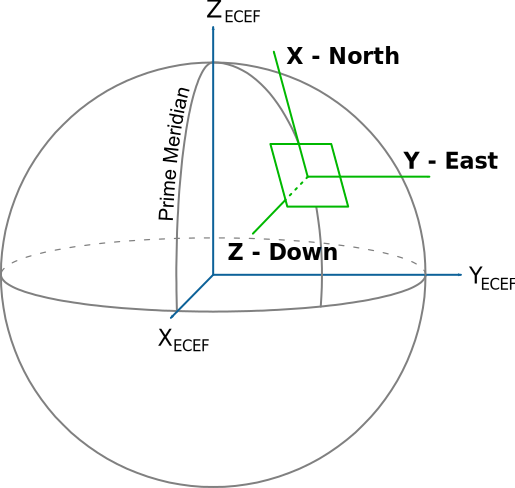
\includegraphics[width=0.45\textwidth]{application/NED_ECEF}
    % The source image is released under CC0, public domain, no attribution required:
    % https://pixabay.com/en/airplane-plane-aircraft-propeller-40374/
    % The final image is drawn by me. The source Inkscape SVG file is located in the same directory.
    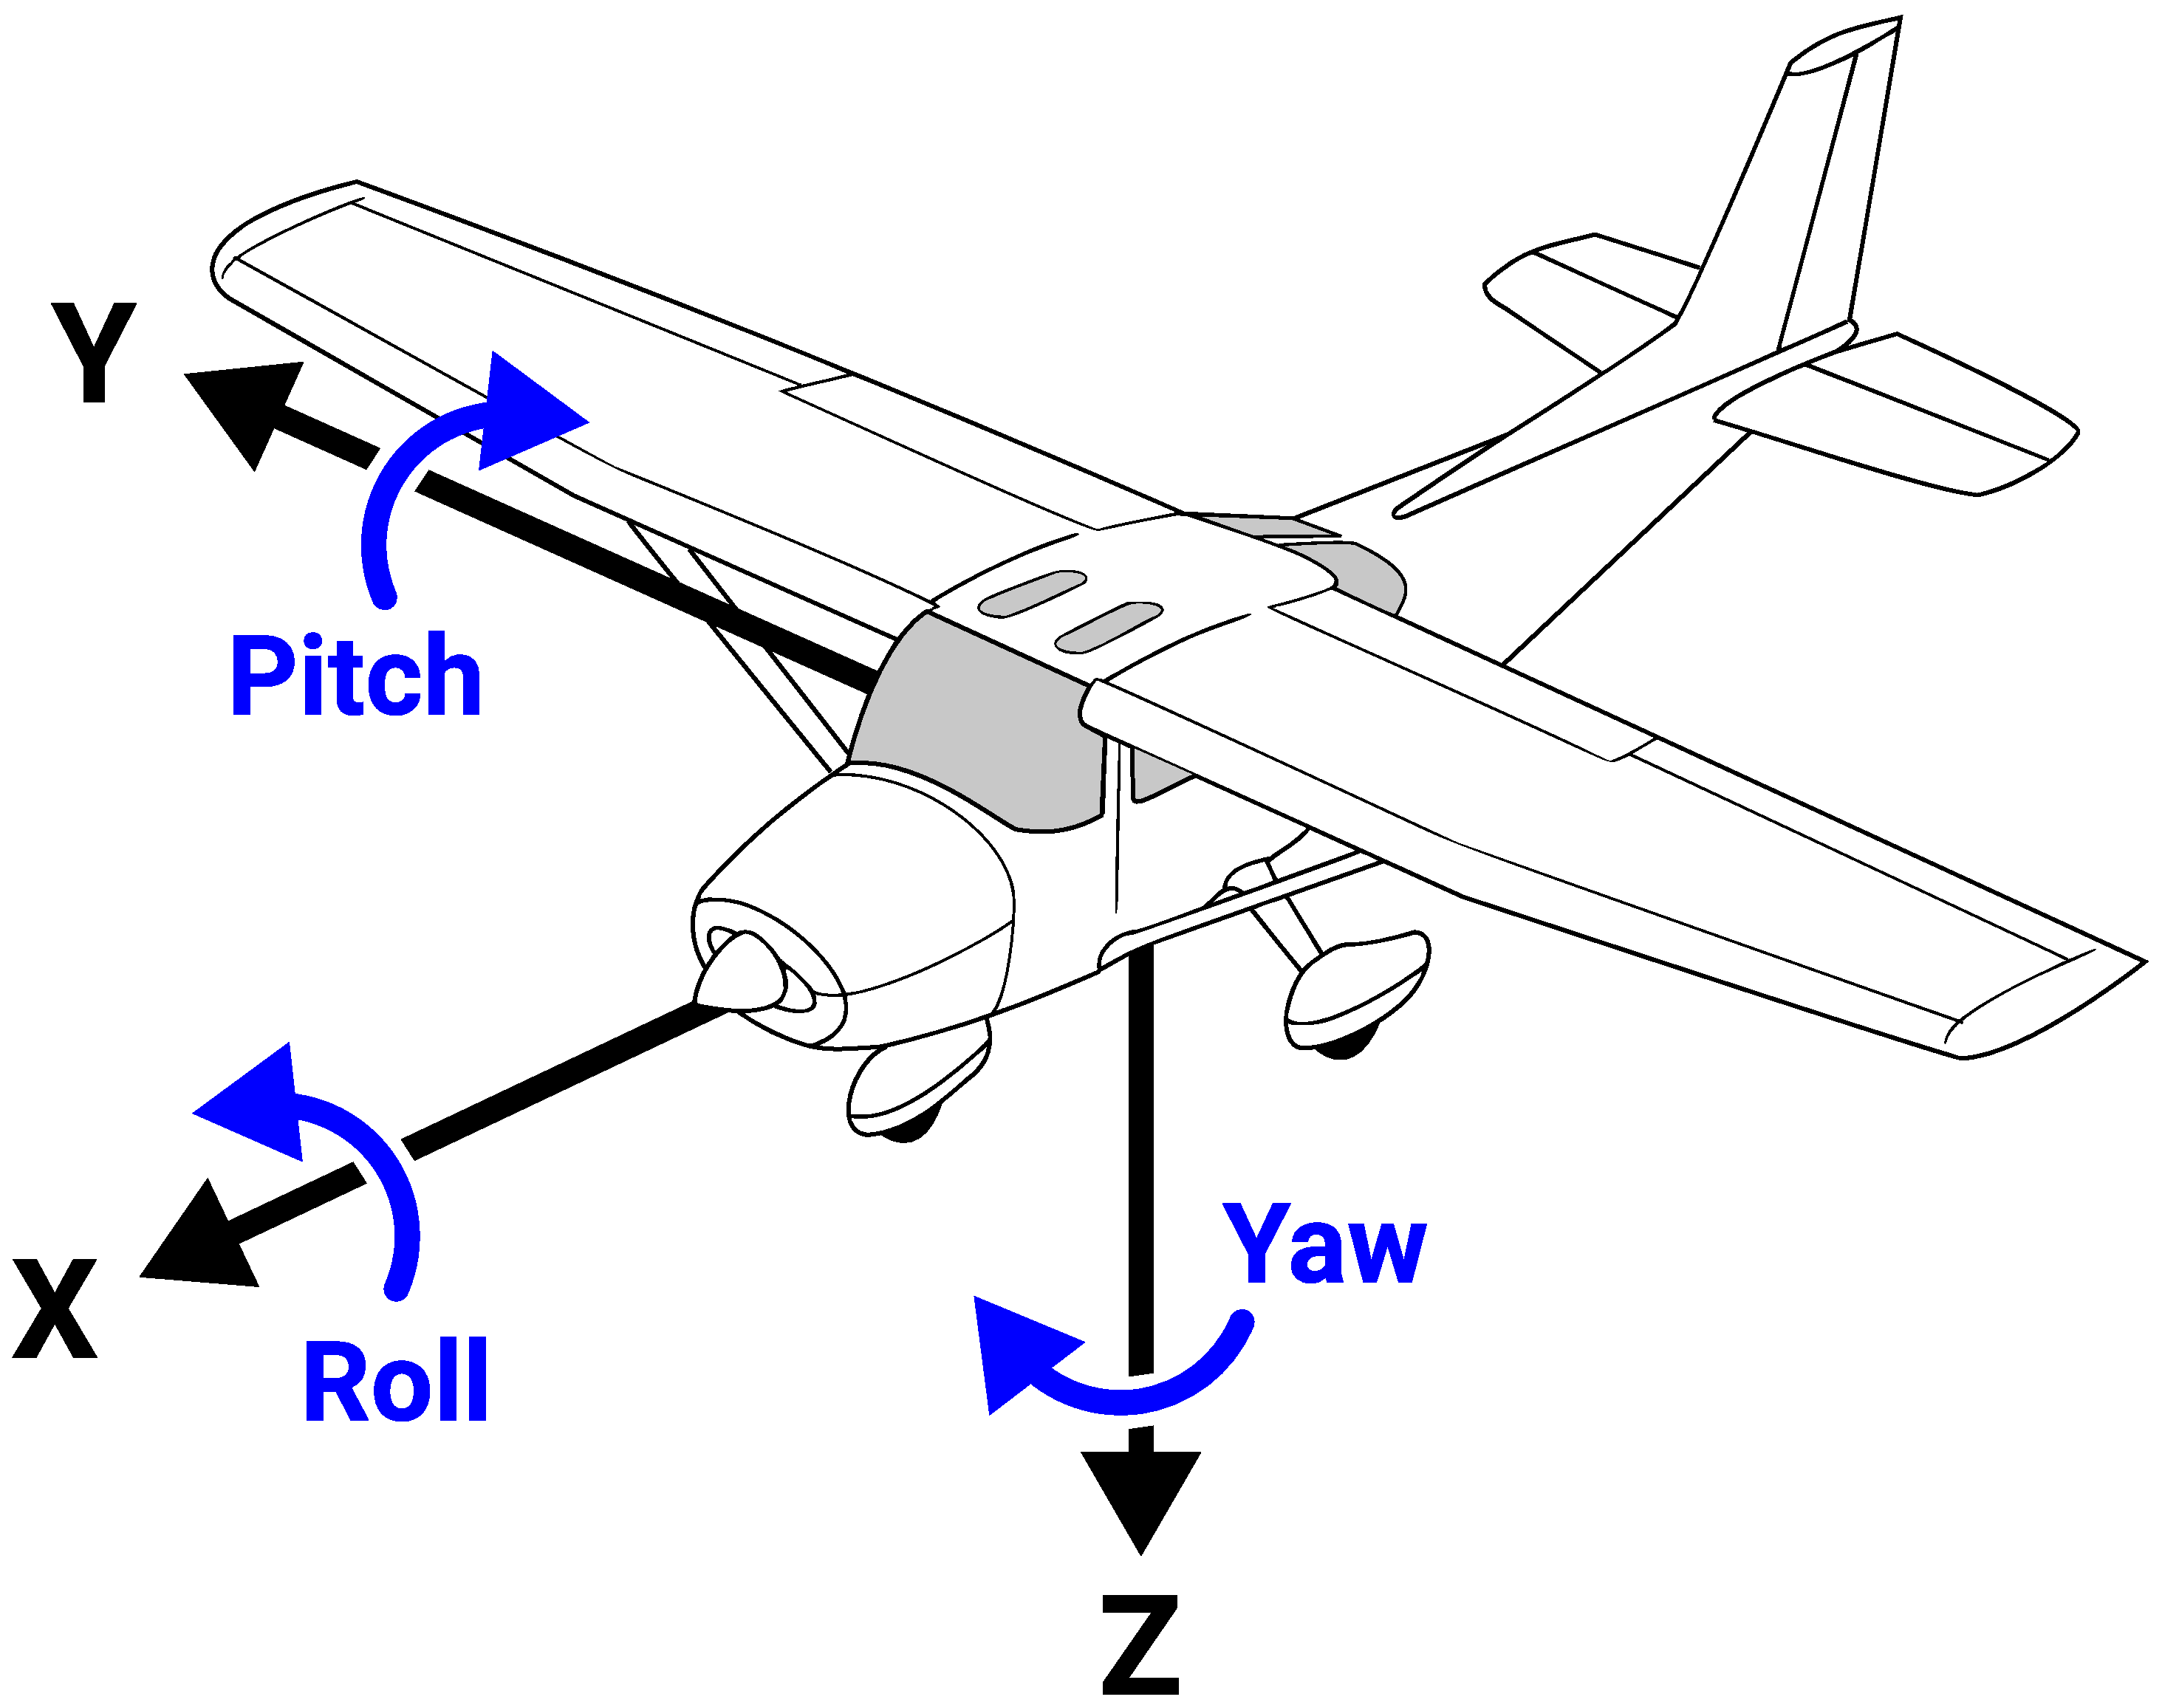
\includegraphics[width=0.45\textwidth]{application/aircraft_principal_axes}
    North-East-Down (NED) frame and body frame conventions. All systems are right-handed.
    \caption{Coordinate frame conventions\label{fig:application_conventions_coordinate_frame}}
\end{figure}

\subsubsection{World frame}

For world fixed frames, the \emph{North-East-Down} (NED) right-handed notation is preferred.
\begin{samepage}
    \begin{description}
        \item[X] --- northward;
        \item[Y] --- eastward;
        \item[Z] --- down.
    \end{description}
\end{samepage}

\subsubsection{Body frame}

In relation to a body, the convention is as defined below, right-handed.
This convention is widely used in aeronautic applications.
\begin{samepage}
    \begin{description}
        \item[X] --- forward;
        \item[Y] --- right;
        \item[Z] --- down.
    \end{description}
\end{samepage}

\subsubsection{Optical frame}

In the case of cameras, the right-handed convention specified below is preferred.
It is widely used in various applications involving computer vision systems.
\begin{samepage}
    \begin{description}
        \item[X] --- right;
        \item[Y] --- down;
        \item[Z] --- towards the scene along the optical axis.
    \end{description}
\end{samepage}

\subsection{Rotation representation}

All applications should represent rotations using quaternions with the elements ordered as follows\footnote{%
    Assuming $w + x\boldsymbol{i} + y\boldsymbol{j} + z\boldsymbol{k}$.
}: W, X, Y, Z.
Other forms of rotation representation should be avoided.

Angular velocities should be represented using the right-handed, fixed-axis (extrinsic) convention:
X (roll), Y (pitch), Z (yaw).

\begin{remark}
    Quaternions are considered to offer the optimal trade-off between bandwidth efficiency,
    computation complexity, and explicitness:
    \begin{itemize}
        \item Euler angles are not self-contained, requiring applications to agree on a particular
              convention beforehand; a convention would be difficult to establish considering different
              demands of various use cases.

        \item Euler angles and fixed axis rotations typically cannot be used for computations directly
              due to angular interpolation issues and singularities; thus, to make use of such
              representations, one often has to convert them to a different form (e.g., quaternion);
              such conversions are computationally heavy.

        \item Rotation matrices are highly redundant.
    \end{itemize}
\end{remark}

\subsection{Matrix representation}

\subsubsection{General}

Matrices should be represented as flat arrays in the row-major order.

\begin{remark}
    $
    \begin{bmatrix}
        x_{11} & x_{12} & x_{13} \\
        x_{21} & x_{22} & x_{23} \\
    \end{bmatrix} \rightarrow \left(x_{11}, x_{12}, x_{13}, x_{21}, x_{22}, x_{23}\right)
    $
\end{remark}

\subsubsection{Square matrices}

There are standard compressed representations of an $n \times n$ square matrix.

An array of size $n^2$ represents a full square matrix.
This is equivalent to the general case reviewed above.

An array of $\frac{(1 + n) n}{2}$ elements represents a symmetric matrix,
where array members represent the elements of the upper-right triangle arranged in the row-major order.
\begin{remark}
    $
    \begin{bmatrix}
        a & b & c \\
        b & d & e \\
        c & e & f \\
    \end{bmatrix} \rightarrow \left(a, b, c, d, e, f\right)
    $

    This form is well-suited for covariance matrix representation.
\end{remark}

An array of $n$ elements represents a diagonal matrix,
where an array member at position $i$ (where $i=1$ for the first element)
represents the matrix element $x_{i, i}$ (where $x_{1, 1}$ is the upper-left element).
\begin{remark}
    $
    \begin{bmatrix}
        a & 0 & 0 \\
        0 & b & 0 \\
        0 & 0 & c \\
    \end{bmatrix} \rightarrow \left(a, b, c\right)
    $
\end{remark}

An array of one element represents a scalar matrix.
\begin{remark}
    $
    \begin{bmatrix}
        a & 0 & 0 \\
        0 & a & 0 \\
        0 & 0 & a \\
    \end{bmatrix} \rightarrow a
    $
\end{remark}

An empty array represents a zero matrix.

\subsubsection{Covariance matrices}

A zero covariance matrix represents an unknown covariance\footnote{%
    As described above, an empty array represents a zero matrix,
    from which follows that an empty array represents unknown covariance.
}.

Infinite error variance means that the associated value is undefined.

\subsection{Physical quantity representation}

\subsubsection{Units}

All units should be SI\footnote{International System of Units.} units (base or derived).
Usage of any other units is strongly discouraged.

When defining data types, fields and constants that represent unscaled quantities in SI units
should not have suffixes indicating the unit, since that would be redundant.

On the other hand, fields and constants that contain quantities in
non-SI units\footnote{E.g., degree Celsius instead of kelvin.}
or scaled SI units\footnote{E.g., microsecond instead of second.}
should be suffixed with the standard abbreviation of the unit\footnote{E.g., kg for kilogram, J for joule.}
and its metric prefix\footnote{E.g., M for mega, n for nano.}
(if any), maintaining the proper letter case of the abbreviation.
In other words, the letter case of the suffix is independent of the letter case of
the attribute it is attached to.

Scaling coefficients should not be chosen arbitrarily;
instead, the choice should be limited to the standard metric prefixes defined by the
International System of Units.

All standard metric prefixes have well-defined abbreviations that are constructed from ASCII characters,
except for one: the micro prefix is abbreviated as a Greek letter ``\textmu{}'' (mu).
When defining data types, ``\textmu{}'' should be replaced with the lowercase Latin letter ``u''.

Irrespective of the suffix, it is recommended to always specify units for every field in the comments.

\begin{remark}
    \begin{minted}{python}
        float16 temperature           # [kelvin] Suffix not needed because an unscaled SI unit is used here.

        uint24 delay_us               # [microsecond] Scaled SI unit, suffix required. Mu replaced with "u".
        uint24 MAX_DELAY_us = 600000  # [microsecond] Notice the letter case.

        float32 kinetic_energy_GJ     # [gigajoule] Notice the letter case.

        float16 estimated_charge_mAh  # [milliampere hour] Scaled non-SI unit. Discouraged, use coulomb.
        float16 MAX_CHARGE_mAh = 1e4  # [milliampere hour] Notice the letter case.
    \end{minted}
\end{remark}

\subsubsection{Enhanced type safety}

In the interest of improving type safety and reducing the possibility of a human error,
it is recommended to avoid reliance on raw scalar types (such as \verb|float32|)
when defining fields containing physical quantities.
Instead, the explicitly typed alternatives defined in the standard DSDL namespace
\DSDLReference{uavcan.si.unit} (also see section~\ref{sec:application_functions_si}) should be used.

\begin{remark}
    \begin{minted}{python}
        float32[4] kinetic_energy                           # [joule] Not recommended.
        uavcan.si.unit.energy.Scalar.1.0[4] kinetic_energy  # This is the recommended practice.
        # Kinetic energy of four bodies.

        float32[3] velocity                                 # [meter/second] Not recommended.
        uavcan.si.unit.velocity.Vector3.1.0                 # This is the recommended practice.
        # 3D velocity vector.
    \end{minted}
\end{remark}

\clearpage\section{Application-level functions}\label{sec:application_level_functions}

This section documents the high-level functionality defined by UAVCAN.
The common high-level functions defined by the specification span across different application domains.
All of the functions defined in this section are optional (not mandatory to implement),
except for the node heartbeat feature (section \ref{sec:application_node_heartbeat}),
which is mandatory for all UAVCAN nodes.

The detailed specifications for each function are provided in the DSDL comments of the data type definitions
they are built upon, whereas this section serves as a high-level overview and index.

\subsection{Node initialization}

UAVCAN does not require that nodes undergo any specific initialization upon connection to the bus ---
a node is free to begin functioning immediately once it is powered up.
The operating mode of the node (such as initialization, normal operation, maintenance, and so on)
is to be reflected via the mandatory heartbeat message described in section \ref{sec:application_node_heartbeat}.

\subsection{Node heartbeat}\label{sec:application_node_heartbeat}

Every non-anonymous UAVCAN node shall report its status and presence by periodically publishing messages of type
\DSDLReference{uavcan.node.Heartbeat} at a fixed rate specified in the message definition using the fixed subject-ID.
Anonymous nodes shall not publish to this subject.

This is the only high-level protocol function that UAVCAN nodes are required to support.
All other data types and application-level functions are optional.

\DSDL{uavcan.node.Heartbeat}

\subsection{Generic node information}

The service \DSDLReference{uavcan.node.GetInfo} can be used to obtain generic information about the node,
such as the structured name of the node (which includes the name of its vendor),
a 128-bit globally unique identifier, the version information about its hardware and software,
version of the UAVCAN specification implemented on the node, and the optional certificate of authenticity.

While the service is, strictly speaking, optional, omitting its support is highly discouraged,
since it is instrumental for network discovery, firmware update, and various maintenance and diagnostic needs.

\DSDL{uavcan.node.GetInfo}

\subsection{Bus data flow monitoring}

The combination of the following three services defined in the namespace \DSDLReference{uavcan.node.port}
(see table \ref{table:dsdl:uavcan.node.port}) enables a highly capable tool of network inspection and monitoring:
\begin{itemize}
    \item \DSDLReference{uavcan.node.port.List} --- designed for obtaining the full set of subjects and services
    implemented by the server node.

    \item \DSDLReference{uavcan.node.port.GetInfo} --- returns the static (unchanging or infrequently changing)
    information about the selected subject or service.

    \item \DSDLReference{uavcan.node.port.GetStatistics} --- returns the transfer event counters of
    the selected subject or service.
\end{itemize}

The first service \verb|List| allows the caller to construct a list of all subjects and services used by the
server node (i.e., the node that the request was sent to).
The second service \verb|GetInfo| allows the caller to map each subject or service to a particular data type,
and understand the role of the server node in relation to said subject or service
(publisher, subscriber, or server).

By comparing the data obtained with the help of these two services from each node on the bus,
the caller can reconstruct the data exchange graph for the entire bus,
thus enabling advanced network monitoring and diagnostics
(assuming that every node on the bus supports the services in question; they are not mandatory).

The last service \verb|GetStatistics| can be used to sample the number of transfers and errors observed
on the specified port.
When invoked periodically, this service allows the caller to observe the real time intensity of data exchange
for each port independently.
In combination with the data exchange graph reconstruction described earlier,
this service allows the caller to build a sophisticated real-time view of the bus.

\DSDL{uavcan.node.port.* --index-only}

\subsection{Network-wide time synchronization}

UAVCAN provides a simple and robust method of time synchronization%
\footnote{The ability to accurately synchronize time between nodes is instrumental for building distributed
real-time data processing systems such as various robotic applications, autopilots, autonomous driving solutions,
and so on.} that is built upon the work
``Implementing a Distributed High-Resolution Real-Time Clock using the CAN-Bus''
published by M.~Gergeleit and H.~Streich%
\footnote{Proceedings of the 1st international CAN-Conference 94, Mainz,
13.-14. Sep. 1994, CAN in Automation e.V., Erlangen.}.
The detailed specification of the time synchronization algorithm is provided in the documentation
for the message type \DSDLReference{uavcan.time.Synchronization}.

\DSDLReference{uavcan.time.GetSynchronizationMasterInfo} provides nodes with information about
the currently used time system and related data like the number of leap seconds added.

Redundant time synchronization masters are supported for the benefit of high-reliability applications.

\begin{remark}
    Time synchronization with explicit sensor feed timestamping should be preferred over inferior alternatives
    such as sensor lag reporting that are sometimes found in simpler systems because such alternatives
    are difficult to scale and they do not account for the delays introduced by communication interfaces.

    It is the duty of every node that publishes timestamped data to account for its own internal delays;
    for example, if the data latency of a local sensor is known,
    it needs to be accounted for in the reported timestamp value.
\end{remark}

\DSDL{uavcan.time.* --index-only}

\subsection{Primitive types and physical quantities}

The namespaces \DSDLReference{uavcan.si} and \DSDLReference{uavcan.primitive}
included in the standard data type set are designed to provide a generic and flexible
method of real-time data exchange. However, these are not bandwidth-efficient.

Generally, applications where the bus bandwidth and latency are important should minimize their reliance
on these generic data types and favor more specialized types instead that are custom-designed for their
particular use cases; e.g., vendor-specific types or application-specific types, either
designed in-house, published by third parties\footnote{As long as the license permits.}, or supplied by
vendors of COTS equipment used in the application.

Vendors of COTS equipment are recommended to ensure that some minimal functionality is available
via these generic types without reliance on their vendor-specific types (if there are any).
This is important for reusability, because some of the systems where such COTS nodes are
to be integrated may not be able to easily support vendor-specific types.

\subsubsection{SI namespace}\label{sec:application_si}

The \verb|si| namespace is named after the International System of Units (SI).
The namespace contains a collection of scalar and vector value types that describe most commonly used
physical quantities in SI; for example, velocity, mass, energy, angle, and time.
The objective of these types is to permit construction of arbitrarily complex distributed control systems without
reliance on any particular vendor-specific data types.

The namespace \DSDLReference{uavcan.si.unit} contains basic units that can be used as type-safe wrappers
over \verb|float32| and other scalar and array types.

The namespace \DSDLReference{uavcan.si.sample} contains time-stamped versions of the above,
where the timestamp field is always located at the end in order to make the time-stamped types
structural sub-types of the non-timestamped ones.
The structural sub-typing enhances interoperability.

Each message type defined in the namespace \verb|uavcan.si.sample| contains a timestamp field of type
\DSDLReference{uavcan.time.SynchronizedTimestamp}.
Every emitted message should be timestamped in order to allow subscribers to identify which of the messages
relate to the same event or to the same instant.
Messages that are emitted in bulk in relation to the same event or the same instant should contain
exactly the same value of the timestamp to simplify the task of timestamp matching for the subscribers.

The exact strategy of matching related messages by timestamp employed by subscribers is entirely
implementation-defined.
The specification does not concern itself with this matter because it is expected that different applications
will opt for different design trade-offs and different tactics to suit their constraints.
Such diversity is not harmful, because its effects are always confined to the local node and cannot affect
operation of other nodes or their compatibility.

The tables \ref{table:dsdl:uavcan.si.unit} and \ref{table:dsdl:uavcan.si.sample}
provide a high-level overview of the SI namespace.
Please follow the references for details.

\DSDL{uavcan.si.unit.* --index-only}

\DSDL{uavcan.si.sample.* --index-only}

\subsubsection{Primitive namespace}

The primitive namespace contains a collection of primitive types:
integer types, floating point types, bit flag, string, raw block of bytes, and an empty value.
Integer, floating point, and bit flag types are available in two categories: scalar and array;
the latter are limited so that their serialized representation is never larger than 257 bytes.

The primitive types are designed to complement the SI namespace with an even simpler set of basic types
that do not make any assumptions about the meaning of the data they describe.
The primitive types provide a very high degree of flexibility, but due to their lack of semantic information,
their use carries the risk of creating suboptimal interfaces that are difficult to use, validate, and scale.

Normally, the use of primitive types should be limited to very basic vendor-neutral interfaces for COTS
equipment and software, debug and diagnostic purposes, and whenever there is a need to exchange data the
type of which cannot be determined statically.\footnote{An example of the latter use case is the register protocol
described in section \ref{sec:application_register_interface}.}

The table \ref{table:dsdl:uavcan.primitive} provides a high-level overview of the primitive namespace.
Please follow the references for details.

\DSDL{uavcan.primitive.* --index-only}

\subsection{Remote file system interface}\label{sec:application_file_system}

The set of standard data types contains a collection of services for manipulation of remote file systems
(namespace \DSDLReference{uavcan.file}, see the table \ref{table:dsdl:uavcan.file}).
All basic file system operations are supported, including file reading and writing,
directory listing, metadata retrieval (size, modification time, etc.), moving, renaming, creating, and deleting.

The set of supported operations may be extended in future versions of the protocol.

Implementers of file servers are strongly advised to always support services \verb|Read| and \verb|GetInfo|,
as that allows clients to make assumptions about the minimal degree of available service.
If write operations are required, all of the defined services should be supported.

\DSDL{uavcan.file.* --index-only}

\subsection{Generic node commands}\label{sec:application_generic_node_commands}

Commonly used node-level application-agnostic auxiliary commands
(such as: restart, power off, factory reset, emergency stop, etc.)
are supported via the standard service \DSDLReference{uavcan.node.ExecuteCommand}.
The service also allows vendors to define vendor-specific commands alongside the standard ones.

It is recommended to support this service in all nodes.

\subsection{Node software update}

A simple software\footnote{Or firmware -- UAVCAN does not distinguish between the two.}
update protocol is defined on top of the remote file system interface (section \ref{sec:application_file_system})
and the generic node commands (section \ref{sec:application_generic_node_commands}).

The software update process involves the following data types:

\begin{itemize}
    \item \DSDLReference{uavcan.node.ExecuteCommand} -- used to initiate the software update process.
    \item \DSDLReference{uavcan.file.Read} -- used to transfer the software image file(s)
          from the file server to the updated node.
\end{itemize}

The software update protocol logic is described in detail in the documentation for the data type
\DSDLReference{uavcan.node.ExecuteCommand}.
The protocol is considered simple enough to be usable in embedded bootloaders with
small memory-constrained microcontrollers.

\subsection{Register interface}\label{sec:application_register_interface}

UAVCAN defines the concept of \emph{named register} -- a scalar, vector, or string value with an associated
human-readable name that is stored on a UAVCAN node locally and is accessible via
UAVCAN\footnote{And, possibly, other interfaces.} for reading and/or modification
by other nodes on the bus.

Named registers are designed to serve the following purposes:
\begin{description}
    \item[Node configuration parameter management] --- Named registers can be used to expose persistently stored
          values that define behaviors of the local node.

    \item[Diagnostics and monitoring] --- Named registers can be used to expose internal states (variables) of
          the node's decision-making and data processing logic (implemented in software or hardware) to provide
          insights about its inner processes.

    \item[Advanced node information reporting] --- Named registers can store any invariants provided by the vendor,
          such as calibration coefficients or unique identifiers.

    \item[Special functions] --- Non-persistent named registers can be used to trigger specific behaviors or
          start predefined operations when written.

    \item[Advanced debugging] --- Registers following a specific naming pattern can be used to provide direct read
          and write access to the local node's application software to facilitate in-depth debugging and monitoring.
\end{description}

The register protocol rests upon two service types defined in the namespace \DSDLReference{uavcan.register};
the namespace index is shown in the table \ref{table:dsdl:uavcan.register}.
Data types supported by the register protocol are defined in the nested data structure
\DSDLReference{uavcan.register.Value}.

The UAVCAN specification defines several standard naming patterns to facilitate cross-vendor compatibility
and provide a framework of common basic functionality.

\DSDL{uavcan.register.* --index-only}

\subsection{Diagnostics and event logging}

The message type \DSDLReference{uavcan.diagnostic.Record} is designed to facilitate emission of
human-readable diagnostic messages and event logging,
both for the needs of real-time display\footnote{E.g., messages displayed to a human operator/pilot in real time.}
and for long-term storage\footnote{E.g., flight data recording.}.

\subsection{Plug-and-play nodes}

Every UAVCAN node shall have a node-ID that is unique within the network (excepting anonymous nodes).
Normally, such identifiers are assigned by the network designer, integrator, some automatic external tool,
or another entity that is external to the network.
However, there exist circumstances where such manual assignment is either difficult or undesirable.

Nodes that can join any UAVCAN network automatically without any prior manual configuration
are called \emph{plug-and-play nodes} (or \emph{PnP nodes} for brevity).

Plug-and-play nodes automatically obtain a node-ID and deduce all necessary parameters of the physical layer
such as the bit rate.

UAVCAN defines an automatic node-ID allocation protocol that is built on top of the data types defined in the
namespace \DSDLReference{uavcan.pnp} (where \emph{pnp} stands for ``plug-and-play'')
(see table \ref{table:dsdl:uavcan.pnp}).
The protocol is described in the documentation for the data type \DSDLReference{uavcan.pnp.NodeIDAllocationData}.

The plug-and-play node-ID allocation protocol relies on anonymous messages reviewed in section
\ref{sec:transport_route_specifier}.
Remember that the plug-and-play feature is entirely optional and it is expected that applications where a
high degree of determinism and robustness is expected are unlikely to benefit from it.

This feature derives from the work
``In search of an understandable consensus algorithm''%
\footnote{Proceedings of USENIX Annual Technical Conference, p. 305-320, 2014.}
by Diego Ongaro and John Ousterhout.

\DSDL{uavcan.pnp.* --index-only}

\subsection{Internet/LAN forwarding interface}

Data types defined in the namespace \DSDLReference{uavcan.internet} (see table \ref{table:dsdl:uavcan.internet})
are designed for establishing robust direct connectivity between local UAVCAN nodes and hosts on the Internet
or on a local area network (LAN) by means of so called \emph{modem nodes}%
\footnote{Normally, a modem node would be implemented using on-board cellular, radio frequency,
or satellite communication hardware.}
(possibly redundant).

This basic support for world-wide communication provided at the protocol level allows any component
of a vehicle equipped with modem nodes to reach external resources or exchange arbitrary data globally
without dependency on application-specific means of communication%
\footnote{Information security and other security-related concerns are outside of the scope of this specification.}.

The set of supported Internet/LAN protocols may be extended in future revisions of the specification.

\begin{remark}
    Some of the major applications for this feature are as follows:
    \begin{enumerate}
        \item Direct telemetry transmission from UAVCAN nodes to a remote data collection server.
        \item Implementation of remote API for on-board equipment (e.g., web interface).
        \item Reception of real-time correction data streams (e.g., RTCM RC-104)
              for precise positioning applications.
        \item Automatic upgrades directly from the vendor's Internet resources.
    \end{enumerate}
\end{remark}

\DSDL{uavcan.internet.* --index-only}

\subsection{Meta-transport}

Data types defined in the namespace \DSDLReference{uavcan.metatransport}
(see table \ref{table:dsdl:uavcan.metatransport})
are designed for tunneling transport frames\footnote{Section \ref{sec:transport_model}.}
over UAVCAN subjects,
as well as logging UAVCAN traffic in the form of serialized UAVCAN message objects.

\DSDL{uavcan.metatransport.* --index-only}


\chapter{Physical layer}\label{sec:physical_layer}

This chapter contains the specification of the supported physical layers of UAVCAN,
as well as some related hardware design recommendations.

Following the requirements and recommendations of this chapter will ensure the highest level of
inter-vendor compatibility and allow the developers to avoid many common design pitfalls.

The sections that provide transport-specific physical layer specification
directly correspond to those defined in the chapter \ref{sec:transport_layer}.

% Please keep \clearpage in front of every transport-specific specification to enforce clear separation!
\clearpage\section{UAVCAN/CAN}\label{sec:transport_can}

\hyphenation{UAVCAN/CAN}  % Disable hyphenation.

This section specifies a concrete transport based on CAN 2.0B (ISO 11898).
Throughout this section, ``CAN'' implies both Classic CAN 2.0 and CAN FD, unless specifically noted otherwise.
CAN FD should be considered the primary transport protocol.

\begin{UAVCANSimpleTable}{UAVCAN/CAN transport capabilities}{|l X l|}
    \label{table:transport_can_capabilities}
    Parameter & Value & References \\

    Maximum node-ID value &
    127 (7 bits wide). &
    \ref{sec:basic} \\

    Transfer-ID mode &
    Cyclic, modulo 32. &
    \ref{sec:transport_transfer_id} \\

    Number of transfer priority levels &
    8 (no additional levels). &
    \ref{sec:transport_transfer_priority} \\

    Largest single-frame transfer payload &
    Classic CAN -- 7~bytes, CAN FD -- up to 63~bytes. &
    \ref{sec:transport_transfer_payload} \\

    Anonymous transfers &
    Supported with non-deterministic collision resolution policy. &
    \ref{sec:transport_route_specifier} \\
\end{UAVCANSimpleTable}

\subsection{CAN ID field}

UAVCAN/CAN transport frames are CAN 2.0B frames.
The 29-bit CAN ID encodes the session specifier\footnote{Section \ref{sec:transport_session_specifier}.}
of the transfer it belongs to along with its priority.
The CAN data field of every frame contains the transfer payload
(or, in the case of multi-frame transfers, a fraction thereof), the transfer-ID, and other metadata.

UAVCAN/CAN can share the same bus with other high-level CAN bus protocols provided that they
do not make use of CAN 2.0B frames\footnote{For example, CANOpen or CANaerospace.}.
However, future revisions of UAVCAN/CAN may utilize CAN 2.0A as well,
so backward compatibility with other high-level CAN bus protocols is not guaranteed.

UAVCAN/CAN can share the same bus with UAVCAN/CAN v0 -- the earlier experimental revision of the protocol
(not recommended for new designs).
The protocol version can be determined at runtime on a per-frame basis as described
in section~\ref{sec:transport_can_toggle_bit}.

UAVCAN/CAN utilizes two different CAN ID bit layouts for message transfers and service transfers.
The bit layouts are summarized on figure~\ref{fig:transport_can_id_structure}.
Tables \ref{table:transport_can_id_fields_message_transfer} and \ref{table:transport_can_id_fields_service_transfer}
summarize the purpose of each field and their permitted values
for message transfers and service transfers, respectively.

% Please do not remove the hard placement specifier [H], it is needed to keep elements ordered.
\begin{figure}[H]
    \centering
    \resizebox{\textwidth}{!}{
        \footnotesize
        \begin{tabular}{|l|c|c|c|c|c|c|c|c|c|c|c|c|c|c|c|c|c|c|c|c|c|c|c|c|c|c|c|c|c|} \hline
            %
            % Message transfer
            %
            \multirow{2}{*}{\textbf{Message}} &
            \multicolumn{4}{c|}{Service, not message} &
            \multicolumn{3}{c|}{Anonymous} &
            \multicolumn{14}{c|}{\multirow{2}{*}{Subject-ID}} &
            \multicolumn{1}{c|}{\multirow{2}{*}{R}} &
            \multicolumn{7}{c|}{\multirow{2}{*}{Source node-ID}}
            \\\cline{2-4} \cline{7-8}

            &
            \multicolumn{3}{c|}{Priority}
            &
            &
            &
            R &
            \multicolumn{15}{c|}{} &
            &
            \multicolumn{7}{c|}{}
            \\

            \textbf{Values} &
            \multicolumn{3}{c|}{$[0, 7]$} &
            $0$ &
            $\mathbb{B}$ &
            $0$ &
            \multicolumn{1}{c}{} &
            \multicolumn{14}{c|}{$[0, 32767]$} &
            $0$ &
            \multicolumn{7}{c|}{$[0, 127]$}
            \\\hline

            \textbf{CAN ID bit} &
            28 & 27 & 26 & 25 & 24 & 23 & 22 & 21 & 20 & 19 & 18 & 17 & 16 & 15 &
            14 & 13 & 12 & 11 & 10 &  9 &  8 &  7 &  6 &  5 &  4 &  3 &  2 &  1 &  0
            \\\hline

            \textbf{CAN ID byte} &
            \multicolumn{5}{c|}{3} & \multicolumn{8}{c|}{2} & \multicolumn{8}{c|}{1} & \multicolumn{8}{c|}{0}
            \\\hline

            \multicolumn{30}{c}{} \\ \hline % Table separator

            %
            % Service transfer
            %
            \multirow{2}{*}{\textbf{Service}} &
            \multicolumn{4}{c|}{Service, not message} &
            \multicolumn{5}{c|}{Request, not response} &
            \multicolumn{6}{c|}{} &
            \multicolumn{7}{c|}{\multirow{2}{*}{Destination node-ID}} &
            \multicolumn{7}{c|}{\multirow{2}{*}{Source node-ID}}
            \\\cline{2-4} \cline{7-10}

            &
            \multicolumn{3}{c|}{Priority} &
            &
            &
            R &
            \multicolumn{9}{c|}{Service-ID} &
            \multicolumn{7}{c|}{} &
            \multicolumn{7}{c|}{}
            \\

            \textbf{Values} &
            \multicolumn{3}{c|}{$[0, 7]$} &
            $1$ &
            $\mathbb{B}$ &
            $0$ &
            \multicolumn{9}{c|}{$[0, 511]$} &
            \multicolumn{7}{c|}{$[0, 127]$} &
            \multicolumn{7}{c|}{$[0, 127]$}
            \\\hline

            \textbf{CAN ID bit} &
            28 & 27 & 26 & 25 & 24 & 23 & 22 & 21 & 20 & 19 & 18 & 17 & 16 & 15 &
            14 & 13 & 12 & 11 & 10 &  9 &  8 &  7 &  6 &  5 &  4 &  3 &  2 &  1 &  0
            \\\hline

            \textbf{CAN ID byte} &
            \multicolumn{5}{c|}{3} & \multicolumn{8}{c|}{2} & \multicolumn{8}{c|}{1} & \multicolumn{8}{c|}{0}
            \\\hline
        \end{tabular}
    }
    \caption{CAN ID bit layout}\label{fig:transport_can_id_structure}
\end{figure}

\begin{UAVCANSimpleTable}{CAN ID bit fields for message transfers}{|l l l X|}
    \label{table:transport_can_id_fields_message_transfer}
    Field               & Width & Valid values  & Description \\

    Transfer priority   & 3     & $[0, 7]$ (any)    & Section \ref{sec:transport_transfer_priority}. \\

    Service not message & 1     & $0$               & Always zero for message transfers. \\

    Anonymous           & 1     & $\{0, 1\}$ (any)  & Zero for regular message transfers,
                                                      one for anonymous transfers. \\

    Reserved bit 23     & 1     & $0$               & Discard frame if this field has a different value. \\

    Subject-ID          & 15    & $[0, 32767]$ (any) & Subject-ID of the current message transfer. \\

    Reserved bit 7      & 1     & $0$               & Discard frame if this field has a different value. \\

    Source node-ID      & 7     & $[0, 127]$ (any)  & Node-ID of the origin.
                                                      For anonymous transfers, this field contains a pseudo-ID instead,
                                                      as described in section
                                                      \ref{sec:transport_can_source_node_pseudo_id}. \\
\end{UAVCANSimpleTable}

\begin{UAVCANSimpleTable}{CAN ID bit fields for service transfers}{|l l l X|}
    \label{table:transport_can_id_fields_service_transfer}
    Field               & Width & Valid values  & Description \\

    Transfer priority   & 3     & $[0, 7]$ (any)    & Section \ref{sec:transport_transfer_priority}. \\

    Service not message & 1     & $1$               & Always one for service transfers. \\

    Request not response& 1     & $\{0, 1\}$ (any)  & One for service request, zero for service response. \\

    Reserved bit 23     & 1     & $0$               & Discard frame if this field has a different value. \\

    Service-ID          & 9     & $[0, 511]$ (any)  & Service-ID of the encoded service object
                                                      (request or response). \\

    Destination node-ID & 7     & $[0, 127]$ (any)  & Node-ID of the destination:
                                                      server if request, client if response. \\

    Source node-ID      & 7     & $[0, 127]$ (any)  & Node-ID of the origin:
                                                      client if request, server if response. \\
\end{UAVCANSimpleTable}

\subsubsection{Transfer priority}

Valid values for transfer priority range from 0 to 7, inclusively,
where 0 corresponds to the highest priority, and 7 corresponds to the lowest priority
(according to the CAN bus arbitration policy).

In multi-frame transfers, the value of the priority field shall be identical for all frames of the transfer.

\begin{remark}[breakable]
    When multiple transfers of different types with the same priority contest for bus access,
    the following precedence is ensured (from higher priority to lower priority):

    \begin{enumerate}
        \item Message transfers (the primary method of data exchange in UAVCAN networks).
        \item Anonymous (message) transfers.
        \item Service response transfers (preempt requests).
        \item Service request transfers (responses take precedence over requests to make service calls more atomic
              and reduce the number of pending states in the system).
    \end{enumerate}

    Mnemonics for transfer priority levels are provided in section \ref{sec:transport_transfer_priority},
    and their mapping to the UAVCAN/CAN priority field is as follows:

    \begin{UAVCANCompactTable}{|l X|}
        Priority field value    & Mnemonic name \\
        0                       & Exceptional   \\
        1                       & Immediate     \\
        2                       & Fast          \\
        3                       & High          \\
        4                       & Nominal       \\
        5                       & Low           \\
        6                       & Slow          \\
        7                       & Optional      \\
    \end{UAVCANCompactTable}

    Since the value of transfer priority is required to be the same for all frames in a transfer,
    it follows that the value of the CAN ID is guaranteed to be the same for all CAN frames of the transfer.
    Given a constant transfer priority value, all CAN frames under a given session specifier will be equal.
\end{remark}

\subsubsection{Source node-ID field in anonymous transfers}\label{sec:transport_can_source_node_pseudo_id}

The source node-ID field of anonymous transfers shall be initialized with a pseudorandom \emph{pseudo-ID} value.
The source of the pseudorandom data used for the pseudo-ID shall aim to produce different values
for different CAN frame data field values.

A node transmitting an anonymous transfer shall abort its transmission and discard it upon detection of a bus error.
Some method of media access control should be used at the application level for further conflict resolution.

\begin{remark}[breakable]
    CAN bus does not allow different nodes to transmit CAN frames with different data under the same CAN ID value.
    Owing to the fact that the CAN ID includes the node-ID of the transmitting node,
    this restriction does not affect non-anonymous transfers.
    However, anonymous transfers would violate this restriction because their source node-ID is not defined,
    hence the additional measures described in this section.

    A possible way of initializing the source node pseudo-ID value is to compute the arithmetic sum
    of all bytes of the transfer payload, taking the least significant bits of the result as the pseudo-ID
    (usage of stronger hashes is encouraged).
    Implementations that adopt this approach will be using the same pseudo-ID value for identical transfer payloads,
    which is acceptable since this will not trigger an error on the bus.

    Because the set of possible pseudo-ID values is small,
    a collision where multiple nodes emit CAN frames with different data but the same CAN ID is likely to happen
    despite the randomization measures described here.
    Therefore, if anonymous transfers are used,
    implementations shall account for possible errors on the CAN bus triggered by CAN ID collisions.

    Automatic retransmission should be disabled for anonymous transfers (like in TTCAN).
    This measure allows the protocol to prevent temporary disruptions that may occur if the automatic
    retransmission on bus error is not suppressed.

    Additional bus access control logic is needed at the application level because
    the possibility of identifier collisions in anonymous frames undermines the access control logic implemented
    in CAN bus controller hardware.

    The described principles make anonymous transfers highly non-deterministic and inefficient.
    This is considered acceptable because the scope of anonymous transfers is limited to a very narrow set of use
    cases which tolerate their downsides. The UAVCAN specification employs anonymous transfers only for the
    plug-and-play feature defined in section \ref{sec:application_functions}.
    Deterministic applications are advised to avoid reliance on anonymous transfers completely.

    None of the above considerations affect nodes that do not transmit anonymous transfers.
\end{remark}

\subsection{CAN data field}

\subsubsection{Layout}

UAVCAN/CAN utilizes a fixed layout of the CAN data field:
the last byte of the CAN data field contains the metadata, it is referred to as the \emph{tail byte}.
The preceding bytes of the data field contain the transfer payload,
which may be extended with padding bytes and transfer CRC.

A CAN frame whose data field contains less than one byte is not a valid UAVCAN/CAN frame.

The bit layout of the tail byte is shown in table \ref{table:transport_can_tail_byte}.

% Please do not remove the hard placement specifier [H], it is needed to keep tables ordered.
\begin{table}[H]\caption{Tail byte structure}\label{table:transport_can_tail_byte}
    \begin{tabu}{| c l | X[c2] X[c3] |}
        \hline
        \rowfont{\bfseries}
        Bit & Field & Single-frame transfers & Multi-frame transfers \\
        \hline
        7   & \textbf{Start of transfer}& Always 1  & First frame: 1, otherwise 0. \\\hline
        6   & \textbf{End of transfer}  & Always 1  & Last frame: 1, otherwise 0. \\\hline
        5   & \textbf{Toggle bit}       & Always 1  & First frame: 1, then alternates;
                                                      section \ref{sec:transport_can_toggle_bit}. \\\hline
        4   &                           & \multicolumn{2}{c|}{} \\
        3   &                           & \multicolumn{2}{c|}{Modulo 32 (range [0, 31])} \\
        2   & \textbf{Transfer-ID}      & \multicolumn{2}{c|}{section \ref{sec:transport_transfer_id}} \\
        1   &                           & \multicolumn{2}{c|}{} \\
        0   &                           & \multicolumn{2}{c|}{\footnotesize{(least significant bit)}} \\
        \hline
    \end{tabu}
\end{table}

\subsubsection{Toggle bit}\label{sec:transport_can_toggle_bit}

Transport frames that form a multi-frame transfer are equipped with a \emph{toggle bit}
which alternates its state every frame within the transfer for frame deduplication purposes\footnote{%
    A frame that appears valid to the receiving node may under certain conditions appear invalid to the transmitter,
    triggering the latter to retransmit the frame, in which case it will be duplicated on the side of the receiver.
}.

\begin{remark}[breakable]
    The toggle bit can be used to facilitate operation of heterogeneous deployments where the experimental
    UAVCAN/CAN v0 shares the same CAN bus with the current version of the standard.

    Whenever a new transfer is initiated, the original state of the toggle bit reflects the protocol version.
    Implementations that need to support simultaneous operation of two versions of the protocol can record
    the state of the toggle bit when the ``start of transfer'' bit is set, and keep this information
    indexed by the value of the CAN ID field (all frames of a transfer are guaranteed to share the same CAN ID).
    The resulting mapping from CAN ID to the protocol version can be used to route incoming frames to the
    implementation of the appropriate version of the protocol.

    \begin{UAVCANSimpleTable}{Protocol version detection based on the toggle bit}{|l l X|}
        Start of transfer   & Toggle bit    & Protocol version \\
        1                   & 0             & UAVCAN v0 (experimental version). \\
        1                   & 1             & UAVCAN v1 (this version). \\
        0                   & x             & Keep the state of the toggle bit from the first frame of the transfer
                                              to detect protocol version in multi-frame transfers. \\
    \end{UAVCANSimpleTable}
\end{remark}

\subsubsection{Transfer payload decomposition}

The transport-layer MTU of Classic CAN-based implementations shall be 8 bytes (the maximum).
The transport-layer MTU of CAN FD-based implementations should be 64 bytes (the maximum).

CAN FD does not guarantee byte-level granularity of the CAN data field length.
If the desired length of the CAN data field cannot be represented due to the granularity constraints,
zero padding bytes are used.

In single-frame transfers, padding bytes are inserted between the end of the payload and the tail byte.

In multi-frame transfers, the transfer payload is appended with trailing zero padding bytes
followed by the transfer CRC (section \ref{sec:transport_can_transfer_crc}).
All transport frames of a multi-frame transfer except the last one shall fully utilize the available
data field capacity; hence, padding is unnecessary there.
The number of padding bytes is computed so that the length granularity constraints
for the last frame of the transfer are satisfied.

\begin{remark}
    Usage of padding bytes implies that when a serialized message is being deserialized by a receiving node,
    the byte sequence used for deserialization may be longer than the actual byte sequence generated by the
    emitting node during serialization.
    This behavior is compatible with the DSDL specification.

    The weak MTU requirement for CAN FD is designed to avoid compatibility issues.
\end{remark}

\subsubsection{Transfer CRC}\label{sec:transport_can_transfer_crc}

Payload of multi-frame transfers is extended with a transfer CRC for validating the correctness of their reassembly.
Transfer CRC is not used with single-frame transfers.

The transfer CRC is computed over the entire payload of the multi-frame transfer
plus the trailing padding bytes, if any.
The resulting CRC value is appended to the transfer payload after the padding bytes (if any)
in the \emph{big-endian byte order} (most significant byte first)\footnote{%
    This is the native byte order for this CRC function.
}.

The CRC function is the standard CRC-16-CCITT:
initial value $\mathrm{FFFF}_{16}$, polynomial $\mathrm{1021}_{16}$,
not reversed, no output XOR, big endian.
The value for an input sequence $\left(49, 50, \ldots, 56, 57\right)$ is $\mathrm{29B1}_{16}$.
The following code snippet provides a basic implementation of the transfer CRC algorithm in C++
(LUT-based alternatives exist).

\begin{samepage}
\begin{minted}{cpp}
#include <cstdint>
#include <cstddef>

/// UAVCAN/CAN transfer CRC function implementation. License: CC0, no copyright reserved.
class CANTransferCRC
{
    std::uint16_t value_ = 0xFFFFU;

public:
    void add(const std::uint8_t byte)
    {
        value_ ^= static_cast<std::uint16_t>(byte) << 8U;
        for (std::uint8_t bit = 8; bit > 0; --bit)
        {
            if ((value_ & 0x8000U) != 0)
            {
                value_ = (value_ << 1U) ^ 0x1021U;
            }
            else
            {
                value_ = value_ << 1U;
            }
        }
    }

    void add(const std::uint8_t* bytes, std::size_t length)
    {
        while (length-- > 0)
        {
            add(*bytes++);
        }
    }

    [[nodiscard]] std::uint16_t get() const { return value_; }
};
\end{minted}
\end{samepage}

\subsection{Examples}

\begin{remark}[breakable]
    Heartbeat from node-ID 42, nominal priority level,
    uptime starting from 0 and then incrementing by one every transfer,
    vendor-specific status code 3471:

    \begin{UAVCANCompactTable}{|l l|}
        CAN ID (hex)      & CAN data (hex)          \\
        \texttt{107D552A} & \texttt{00 00 00 00 04 78 68 E0} \\
        \texttt{107D552A} & \texttt{01 00 00 00 04 78 68 E1} \\
        \texttt{107D552A} & \texttt{02 00 00 00 04 78 68 E2} \\
        \texttt{107D552A} & \texttt{03 00 00 00 04 78 68 E3} \\
    \end{UAVCANCompactTable}

    \verb|uavcan.primitive.String.1.0| under subject-ID 4919 ($1337_{16}$) published by an anonymous node,
    the string is ``\verb|Hello world!|'' (ASCII); one byte of zero padding can be seen between
    the payload and the tail byte:

    \begin{UAVCANCompactTable}{|l l|}
        CAN ID (hex)      & CAN data (hex)                                           \\
        \texttt{11133775} & \texttt{00 18 48 65 6C 6C 6F 20 77 6F 72 6C 64 21 00 E0} \\
        \texttt{11133775} & \texttt{00 18 48 65 6C 6C 6F 20 77 6F 72 6C 64 21 00 E1} \\
        \texttt{11133775} & \texttt{00 18 48 65 6C 6C 6F 20 77 6F 72 6C 64 21 00 E2} \\
        \texttt{11133775} & \texttt{00 18 48 65 6C 6C 6F 20 77 6F 72 6C 64 21 00 E3} \\
    \end{UAVCANCompactTable}

    Node info request from node 123 to node 42 via Classic CAN, then response;
    notice how the transfer CRC is scattered across two frames:

    \begin{UAVCANCompactTable}{|l l l X|}
        CAN ID (hex)      & CAN data (hex)                                  & ASCII             & Comment \\

        \texttt{136B957B} & \texttt{E1}                                     & \texttt{.}        &
        The request contains no payload. \\

        \texttt{126BBDAA} & \texttt{01 00 00 00 01 00 00 A1}                & \texttt{........} &
        Start of response, toggle bit is set. \\

        \texttt{126BBDAA} & \texttt{00 00 00 00 00 00 00 01}                & \texttt{........} &
        Toggle bit is cleared. \\

        \texttt{126BBDAA} & \texttt{00 00 00 00 00 00 00 21}                & \texttt{.......!} &
        Toggle bit is set. \\

        \texttt{126BBDAA} & \texttt{00 00 00 00 00 00 00 01}                & \texttt{........} &
        Etc. \\

        \texttt{126BBDAA} & \texttt{00 00 \underline{24} 6F 72 67 2E 21}    & \texttt{..\underline{\$}org.!} &
        Array (string) length prefix. \\

        \texttt{126BBDAA} & \texttt{75 61 76 63 61 6E 2E 01}                & \texttt{uavcan..} &
        \\

        \texttt{126BBDAA} & \texttt{70 79 75 61 76 63 61 21}                & \texttt{pyuavca!} &
        \\

        \texttt{126BBDAA} & \texttt{6E 2E 64 65 6D 6F 2E 01}                & \texttt{n.demo..} &
        \\

        \texttt{126BBDAA} & \texttt{62 61 73 69 63 5F 75 21}                & \texttt{basic\_u!} &
        \\

        \texttt{126BBDAA} & \texttt{73 61 67 65 00 00 \underline{9A} 01}    & \texttt{sage..\underline{.}.} &
        Transfer CRC, MSB. \\

        \texttt{126BBDAA} & \texttt{\underline{E7} 61}                      & \texttt{\underline{.}a}       &
        Transfer CRC, LSB. \\
    \end{UAVCANCompactTable}

    \verb|uavcan.primitive.array.Natural8.1.0| under subject-ID 4919 ($1337_{16}$) published by node 59,
    the array contains an arithmetic sequence $\left(0, 1, 2, \ldots{}, 89, 90, 91\right)$;
    the transport MTU is 64 bytes:

    \begin{UAVCANCompactTable}{|l X[2] X|}
        CAN ID (hex)      & CAN data (hex) & Comment \\
        \texttt{1013373B} &
        \texttt{%
            00 B8 00 01 02 03 04 05 06 07 08 09 0A 0B 0C 0D 0E 0F 10 11 12 13 14 15 16 17 18 19 1A 1B 1C 1D 1E 1F 20
            21 22 23 24 25 26 27 28 29 2A 2B 2C 2D 2E 2F 30 31 32 33 34 35 36 37 38 39 3A 3B 3C A0
        } &
        First frame: 1.~payload (array length prefix is 92); 2.~tail byte. \\

        \texttt{1013373B} &
        \texttt{%
            3D 3E 3F 40 41 42 43 44 45 46 47 48 49 4A 4B 4C 4D 4E 4F 50 51 52 53 54 55 56 57 58 59 5A 5B
            \underline{00} \underline{00} \underline{00} \underline{00} \underline{00} \underline{00} \underline{00}
            \underline{00} \underline{00} \underline{00} \underline{00} \underline{00} \underline{00} \underline{00}
            \textbf{C0} \textbf{48} 40
        } &
        Last frame: 1.~payload; 2.~padding (underlined); 3.~transfer CRC (bold); 4.~tail byte. \\
    \end{UAVCANCompactTable}
\end{remark}

\subsection{Software design considerations}

\subsubsection{Ordered transmission}

The CAN controller driver software shall guarantee that CAN frames with identical CAN ID values
will be transmitted in their order of appearance in the transmission queue\footnote{%
    This is because multi-frame transfers use identical CAN ID for all frames of the transfer,
    and UAVCAN requires that all frames of a multi-frame transfer shall be transmitted in the correct order.
}.

\subsubsection{Transmission timestamping}

\begin{remark}[breakable]
    Certain application-level functions of UAVCAN may require the driver to timestamp outgoing transport frames,
    e.g., the time synchronization function.
    A sensible approach to transmission timestamping is built around the concept of \emph{loop-back frames},
    which is described here.

    If the application needs to timestamp an outgoing frame, it sets a special flag -- the \emph{loop-back flag} --
    on the frame before sending it to the driver.
    The driver would then automatically re-enqueue this frame back into the reception queue once it is transmitted
    (keeping the loop-back flag set so that the application is able to distinguish the loop-back
    frame from regular received traffic).
    The timestamp of the loop-backed frame would be of the moment when it was delivered to the bus.

    The advantage of the loop-back based approach is that it relies on the same interface between
    the application and the driver that is used for regular communications.
    No complex and dangerous callbacks or write-backs from interrupt handlers are involved.
\end{remark}

\subsubsection{Inner priority inversion}

Implementations should take necessary precautions against the problem of inner priority inversion.

\begin{remark}[breakable]
    Suppose the application needs to emit a frame with the CAN ID $X$.
    The frame is submitted to the CAN controller's registers and the transmission is started.
    Suppose that afterwards it turned out that there is a new frame with the CAN ID $(X-1)$ that needs to be sent,
    too, but the previous frame $X$ is in the way, and it is blocking the transmission of the new frame.
    This may turn into a problem if the lower-priority frame is losing arbitration on the bus due
    to the traffic on the bus having higher priority than the current frame,
    but lower priority than the next frame that is waiting in the queue.

    A naive solution to this is to continuously check whether the priority of the frame that is currently being
    transmitted by the CAN controller is lower than the priority of the next frame in the queue, and if it is,
    abort transmission of the current frame, move it back to the transmission queue,
    and begin transmission of the new one instead.
    This approach, however, has a hidden race condition:
    the old frame may be aborted at the moment when it has already been received by remote nodes,
    which means that the next time it is re-transmitted, the remote nodes will see it duplicated.
    Additionally, this approach increases the complexity of the driver and can possibly affect
    its throughput and latency.

    Most CAN controllers offer a robust solution to the problem:
    they have multiple transmission mailboxes (usually at least 3),
    and the controller always chooses for transmission the mailbox which contains the highest priority frame.
    This provides the application with a possibility to avoid the inner priority inversion problem:
    whenever a new transmission is initiated, the application should check whether the priority of the next frame
    is higher than any of the other frames that are already awaiting transmission.
    If there is at least one higher-priority frame pending,
    the application doesn't move the new one to the controller's transmission mailboxes,
    it remains in the queue.
    Otherwise, if the new frame has a higher priority level than all of the pending frames,
    it is pushed to the controller's transmission mailboxes and removed from the queue.
    In the latter case, if a lower-priority frame loses arbitration,
    the controller would postpone its transmission and try transmitting the higher-priority one instead.
    That resolves the problem.

    There is an interesting extreme case, however.
    Imagine a controller equipped with $N$ transmission mailboxes.
    Suppose the application needs to emit $N$ frames in the increasing order of priority,
    which leads to all of the transmission mailboxes of the controller being occupied.
    Now, if all of the conditions below are satisfied, the system ends up with a priority inversion condition
    nevertheless, despite the measures described above:

    \begin{itemize}
        \item The highest-priority pending CAN frame cannot be transmitted due to the bus being saturated
        with a higher-priority traffic.
        \item The application needs to emit a new frame which has a higher priority than that which saturates the bus.
    \end{itemize}

    If both hold, a priority inversion is afoot because there is no free transmission mailbox to
    inject the new higher-priority frame into.
    The scenario is extremely unlikely, however;
    it is also possible to construct the application in a way that would preclude the problem,
    e.g., by limiting the number of simultaneously used distinct CAN ID values.

    The following pseudocode demonstrates the principles explained above:

    \begin{samepage}
    \begin{minted}{cpp}
    // Returns the index of the TX mailbox that can be used for the transmission of the newFrame
    // If none are available, returns -1.
    getFreeMailboxIndex(newFrame)
    {
        chosen_mailbox = -1     // By default, assume that no mailboxes are available

        for i = 0...NumberOfTxMailboxes
        {
            if isTxMailboxFree(i)
            {
                chosen_mailbox = i
                // Note: cannot break here, shall check all other mailboxes as well.
            }
            else
            {
                if not isFramePriorityHigher(newFrame, getFrameFromTxMailbox(i))
                {
                    chosen_mailbox = -1
                    break   // Denied - shall wait until this mailbox has finished transmitting
                }
            }
        }

        return chosen_mailbox
    }
    \end{minted}
    \end{samepage}
\end{remark}

\subsubsection{Automatic hardware acceptance filter configuration}

\begin{remark}[breakable]
    Most CAN controllers are equipped with hardware acceptance filters.
    Hardware acceptance filters reduce the application workload by ignoring irrelevant CAN frames on the bus
    by comparing their ID values against the set of relevant ID values configured by the application.

    There exist two common approaches to CAN hardware filtering:
    list-based and mask-based.
    In the case of the list-based approach, every CAN frame detected on the bus is compared
    against the set of reference CAN ID values provided by the application;
    only those frames that are found in the reference set are accepted.
    Due to the complex structure of the CAN ID field used by UAVCAN,
    usage of the list-based filtering method with this protocol is impractical.

    Most CAN controller vendors implement mask-based filters,
    where the behavior of each filter is defined by two parameters: the mask $M$ and the reference ID $R$.
    Then, such filter accepts only those CAN frames for which the following bitwise logical condition holds
    true\footnote{Notation: $\land$ -- bitwise logical AND, $\oplus$ -- bitwise logical XOR,
    $\neg$ -- bitwise logical NOT.}:
    $$((X \land M) \oplus R) \leftrightarrow 0$$
    where $X$ is the CAN ID value of the evaluated frame.

    Complex UAVCAN applications are often required to operate with more distinct transfers than there are
    acceptance filters available in the hardware.
    That creates the challenge of finding the optimal configuration of the available filters that meets the
    following criteria:
    \begin{itemize}
        \item All CAN frames needed by the application are accepted.
        \item The number of irrelevant frames (i.e., not used by the application) accepted from the bus is minimized.
    \end{itemize}

    The optimal configuration is a function of the number of available hardware filters,
    the set of distinct transfers needed by the application,
    and the expected frequency of occurrence of all possible distinct transfers on the bus.
    The latter is important because if there are to be irrelevant transfers,
    it makes sense to optimize the configuration so that the acceptance of less common irrelevant transfers
    is preferred over the more common irrelevant transfers, as that reduces the processing load on the application.

    The optimal configuration depends on the properties of the network the node is connected to.
    In the absence of the information about the network,
    or if the properties of the network are expected to change frequently,
    it is possible to resort to a quasi-optimal configuration which assumes that
    the occurrence of all possible irrelevant transfers is equally probable.
    As such, the quasi-optimal configuration is a function of only the number of available hardware filters
    and the set of distinct transfers needed by the application.

    The quasi-optimal configuration can be easily found automatically.
    Certain implementations of the UAVCAN protocol stack include this functionality,
    allowing the application to easily adjust the configuration of the hardware acceptance filters
    using a very simple API.

    A quasi-optimal hardware acceptance filter configuration algorithm is described below.
    The approach was first proposed by P. Kirienko and I. Sheremet in 2015.

    First, the bitwise \emph{filter merge} operation is defined on filter configurations $A$ and $B$.
    The set of CAN frames accepted by the merged filter configuration is a superset of
    those accepted by $A$ and $B$.
    The definition is as follows:
    \begin{equation*}
    \begin{split}
        m_M(R_A, R_B, M_A, M_B) & = M_A \land M_B \land \neg (R_A \oplus R_B) \\
        m_R(R_A, R_B, M_A, M_B) & = R_A \land m_M(R_A, R_B, M_A, M_B)
    \end{split}
    \end{equation*}

    The \emph{filter rank} is a function of the mask of the filter.
    The rank of a filter is a unitless quantity that defines in relative terms how selective the filter
    configuration is.
    The rank of a filter is proportional to the likelihood that the filter will reject a random CAN ID.
    In the context of hardware filtering, this quantity is conveniently representable via the number of bits set in
    the filter mask parameter (also known as \emph{population count}):
    \begin{equation*}
    r(M) =
    \begin{cases}
        0                                   &\mid M < 1 \\
        r(\lfloor\frac{M}{2}\rfloor)        &\mid M \bmod 2 = 0 \\
        r(\lfloor\frac{M}{2}\rfloor) + 1    &\mid M \bmod 2 \neq 0 \\
    \end{cases}
    \end{equation*}

    Having the low-level operations defined, we can proceed to define the whole algorithm.
    First, construct the initial set of CAN acceptance filter configurations
    according to the requirements of the application.
    Then, as long as the number of configurations in the set exceeds the number of available
    hardware acceptance filters, repeat the following:
    \begin{enumerate}
        \item Find the pair $A$, $B$ of configurations in the set for which $r(m_M(R_A, R_B, M_A, M_B))$ is maximized.
        \item Remove $A$ and $B$ from the set of configurations.
        \item Add a new configuration $X$ to the set of configurations, where
        $M_X = m_M(R_A, R_B, M_A, M_B)$, and $R_X = m_R(R_A, R_B, M_A, M_B)$.
    \end{enumerate}

    The algorithm reduces the number of filter configurations by one at each iteration,
    until the number of available hardware filters is sufficient to accommodate the whole set of configurations.
\end{remark}


\clearpage
\section{Hardware design recommendations}

This section contains certain generic hardware design recommendations that are agnostic of a particular
physical layer implementation.

\subsection{Nonuniform transport redundancy}\label{sec:phy_nonuniform_transport_redundancy}

Mission critical devices and non-mission critical devices often need to co-exist within the same UAVCAN network.
Non-mission critical devices are likely to be equipped with a non-redundant transport interface,
which can create a situation where multiple devices with different numbers of redundant interfaces
need to be connected to the same network.
In that case, the following rules should be followed:

\begin{itemize}
    \item Each available transport network is assigned a level of importance (primary, secondary, etc.).
    \item All nodes should be connected to the primary transport network.
    \item Only nodes with redundant interfaces should be also connected to the non-primary transport network(s).
\end{itemize}

The figure \ref{fig:phy_nonuniform_transport_redundancy} shows a doubly redundant network as an example.

\begin{figure}[H]
    \centering
	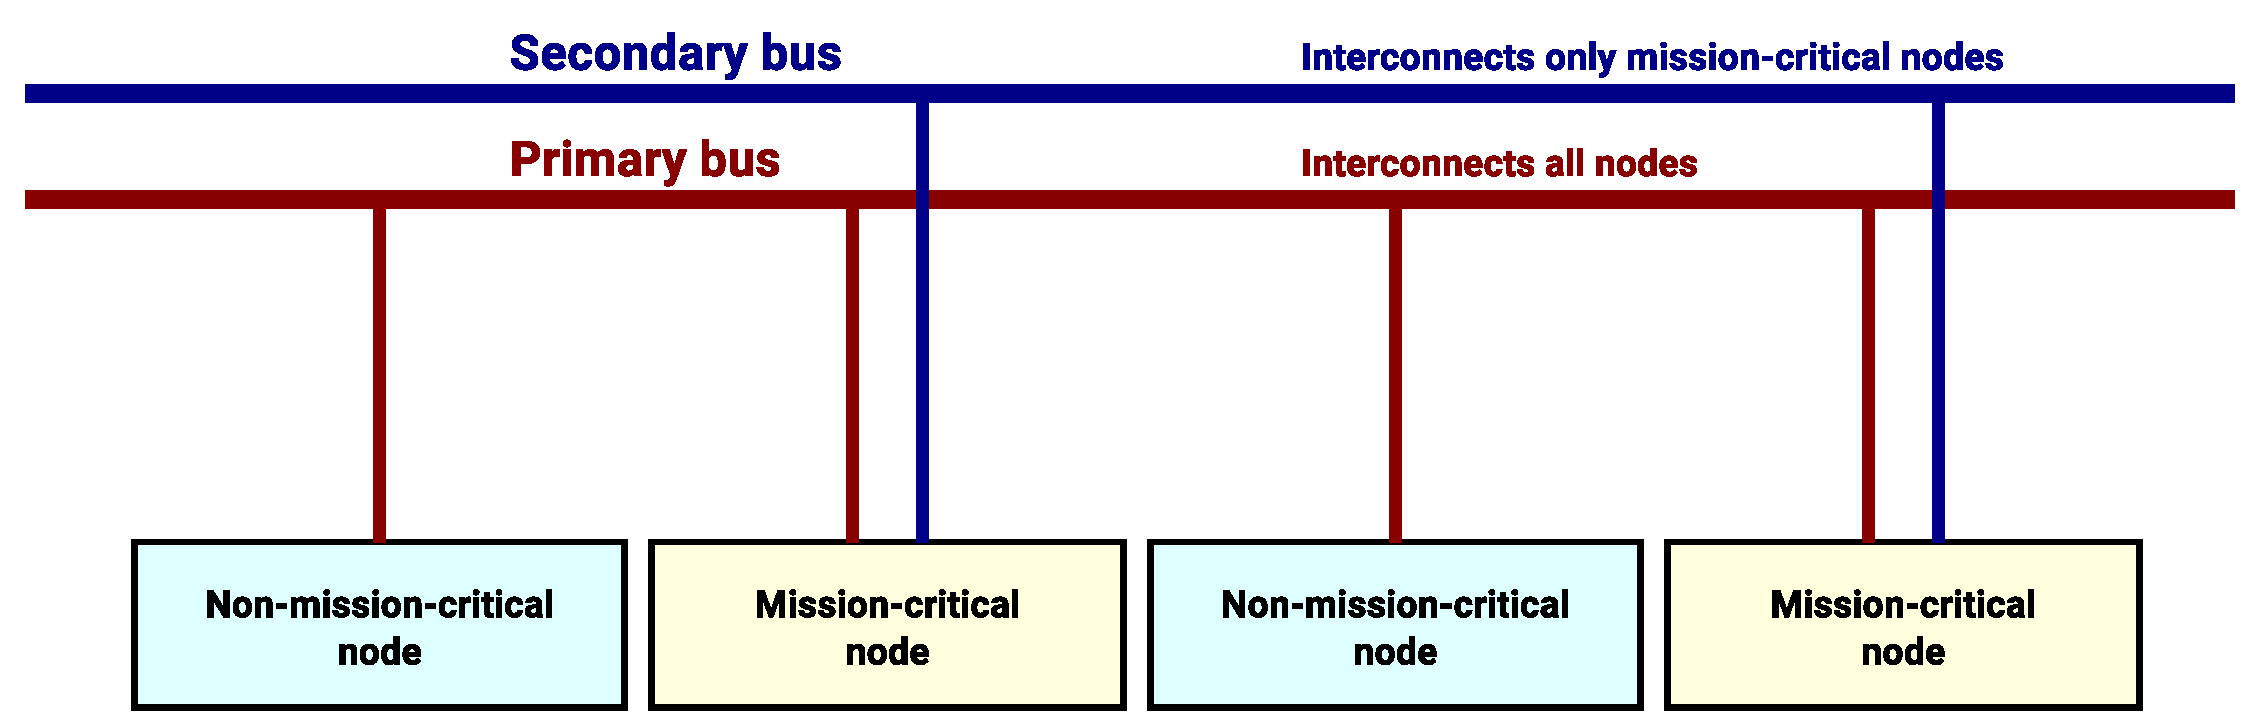
\includegraphics[width=\textwidth]{physical_layer/nonuniform_bus_redundancy}
	\caption{Nonuniform transport redundancy.\label{fig:phy_nonuniform_transport_redundancy}}
\end{figure}

\subsection{Bus power supply}

The standard UAVCAN physical layers support power distribution between nodes.
Integration of the power distribution functionality with the communication interface
removes the need for a dedicated power distribution network,
which greatly simplifies the system design and reduces the complexity and weight of the wiring harnesses.
Additionally, redundant power supply topologies can be easily implemented on top of redundant communication interfaces.

\subsubsection{Power sinking nodes}

This section applies to nodes that draw power from the network.

Each power input should be protected with an over-current protection circuit (for example, an electronic fuse),
so that a short-circuit or a similar failure of the node does not propagate to the entire bus.

If the node incorporates redundant bus interfaces,
it should prevent direct current flow between power inputs from different interface connectors,
so if one bus suffers a power failure (e.g. a short circuit) it is not propagated to the other buses.

\begin{figure}[H]
    \centering
	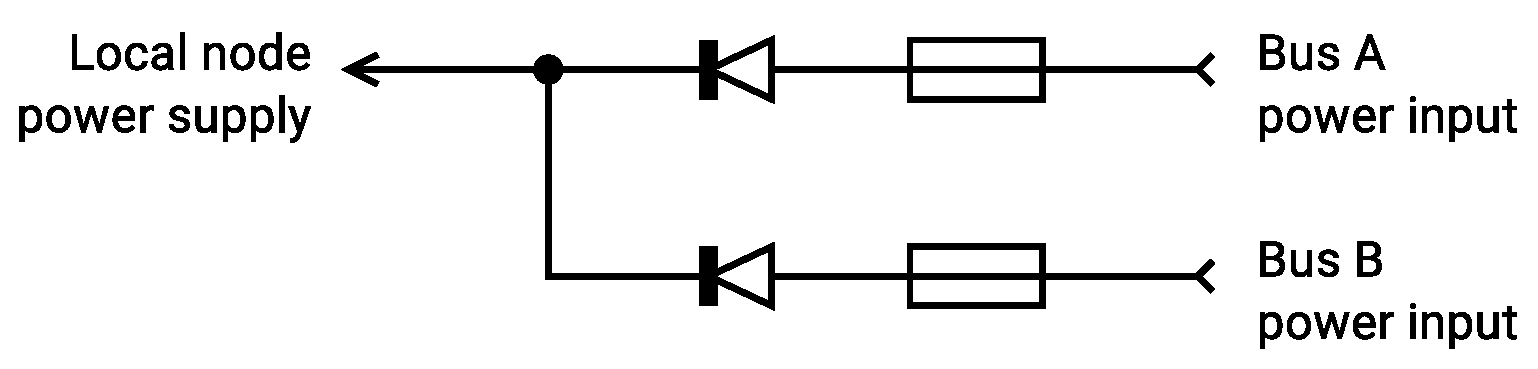
\includegraphics[width=0.6\textwidth]{physical_layer/redundant_bus_power_sink}
	\caption{Simplified conceptual power sinking node design schematic.\label{fig:phy_redundant_bus_power_sink}}
\end{figure}

\subsubsection{Power sourcing nodes}

This section applies to nodes that deliver power to the network.

Similar to the case of bus-powered nodes,
UAVCAN power sources should take into account that one of the redundant interfaces may suffer a
short-circuit or a failure of a similar mode.
Should that happen, the power source should shut down the power supply of the failing bus and continue supplying
the remaining bus interfaces.

\begin{figure}[H]
    \centering
	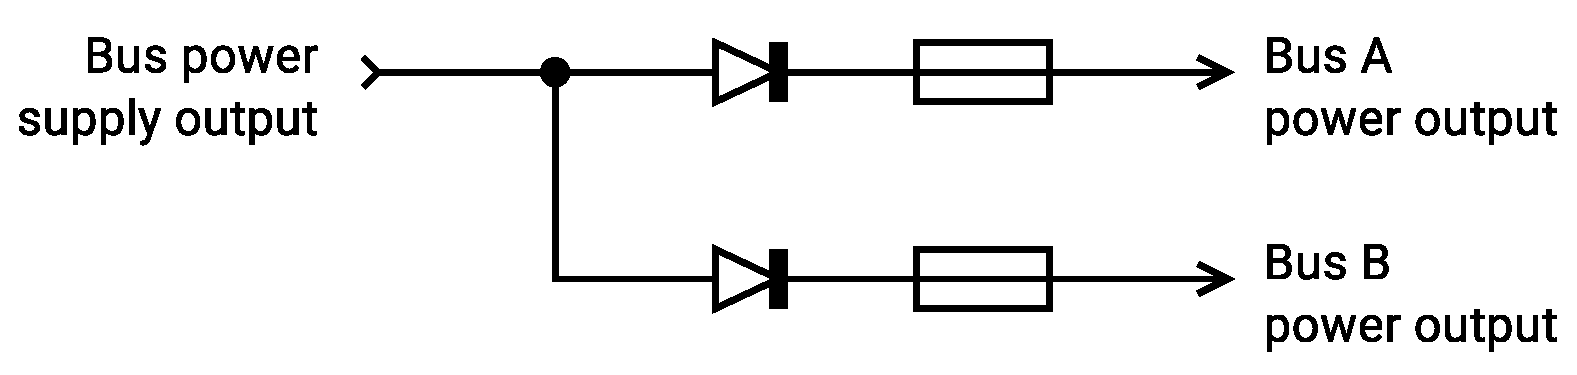
\includegraphics[width=0.6\textwidth]{physical_layer/redundant_bus_power_source}
	\caption{Simplified conceptual power sourcing node design schematic.\label{fig:phy_redundant_bus_power_source}}
\end{figure}


\end{document}
